% Options for packages loaded elsewhere
\PassOptionsToPackage{unicode}{hyperref}
\PassOptionsToPackage{hyphens}{url}
%
\documentclass[
  a4paper,
]{scrbook}

\usepackage{amsmath,amssymb}
\usepackage{lmodern}
\usepackage{iftex}
\ifPDFTeX
  \usepackage[T1]{fontenc}
  \usepackage[utf8]{inputenc}
  \usepackage{textcomp} % provide euro and other symbols
\else % if luatex or xetex
  \usepackage{unicode-math}
  \defaultfontfeatures{Scale=MatchLowercase}
  \defaultfontfeatures[\rmfamily]{Ligatures=TeX,Scale=1}
  \setmainfont[]{Latin Modern Roman}
  \setsansfont[]{Latin Modern Roman}
\fi
% Use upquote if available, for straight quotes in verbatim environments
\IfFileExists{upquote.sty}{\usepackage{upquote}}{}
\IfFileExists{microtype.sty}{% use microtype if available
  \usepackage[]{microtype}
  \UseMicrotypeSet[protrusion]{basicmath} % disable protrusion for tt fonts
}{}
\makeatletter
\@ifundefined{KOMAClassName}{% if non-KOMA class
  \IfFileExists{parskip.sty}{%
    \usepackage{parskip}
  }{% else
    \setlength{\parindent}{0pt}
    \setlength{\parskip}{6pt plus 2pt minus 1pt}}
}{% if KOMA class
  \KOMAoptions{parskip=half}}
\makeatother
\usepackage{xcolor}
\setlength{\emergencystretch}{3em} % prevent overfull lines
\setcounter{secnumdepth}{5}
% Make \paragraph and \subparagraph free-standing
\ifx\paragraph\undefined\else
  \let\oldparagraph\paragraph
  \renewcommand{\paragraph}[1]{\oldparagraph{#1}\mbox{}}
\fi
\ifx\subparagraph\undefined\else
  \let\oldsubparagraph\subparagraph
  \renewcommand{\subparagraph}[1]{\oldsubparagraph{#1}\mbox{}}
\fi


\providecommand{\tightlist}{%
  \setlength{\itemsep}{0pt}\setlength{\parskip}{0pt}}\usepackage{longtable,booktabs,array}
\usepackage{calc} % for calculating minipage widths
% Correct order of tables after \paragraph or \subparagraph
\usepackage{etoolbox}
\makeatletter
\patchcmd\longtable{\par}{\if@noskipsec\mbox{}\fi\par}{}{}
\makeatother
% Allow footnotes in longtable head/foot
\IfFileExists{footnotehyper.sty}{\usepackage{footnotehyper}}{\usepackage{footnote}}
\makesavenoteenv{longtable}
\usepackage{graphicx}
\makeatletter
\def\maxwidth{\ifdim\Gin@nat@width>\linewidth\linewidth\else\Gin@nat@width\fi}
\def\maxheight{\ifdim\Gin@nat@height>\textheight\textheight\else\Gin@nat@height\fi}
\makeatother
% Scale images if necessary, so that they will not overflow the page
% margins by default, and it is still possible to overwrite the defaults
% using explicit options in \includegraphics[width, height, ...]{}
\setkeys{Gin}{width=\maxwidth,height=\maxheight,keepaspectratio}
% Set default figure placement to htbp
\makeatletter
\def\fps@figure{htbp}
\makeatother

\usepackage{booktabs}
\usepackage{longtable}
\usepackage{array}
\usepackage{multirow}
\usepackage{wrapfig}
\usepackage{float}
\usepackage{colortbl}
\usepackage{pdflscape}
\usepackage{tabu}
\usepackage{threeparttable}
\usepackage{threeparttablex}
\usepackage[normalem]{ulem}
\usepackage{makecell}
\usepackage{xcolor}
\usepackage{titling}
\setlength{\droptitle}{-2cm}
\preauthor{
  \begin{center}
  \Large
  \vspace{10mm}
  by

  \vspace{20mm}
}
\postauthor{
  \end{center}
  \vfill
}

\predate{
  \begin{center}
  A thesis 
  submitted in fulfilment of the \\
  requirements of the degree of \\
  Doctor of Philosophy in Physics\\               % Degree
  School of Physical and Chemical Sciences\\          % Department
  Te Herenga Waka - Victoria University of Wellington\\                       % University 
  \vspace{5mm}
}
\postdate{
  \\
  
\includegraphics[width=3in,height=1.5in]{figures/VUW-logo.png}\\
  \end{center}
  }
\makeatletter
\makeatother
\makeatletter
\@ifpackageloaded{bookmark}{}{\usepackage{bookmark}}
\makeatother
\makeatletter
\@ifpackageloaded{caption}{}{\usepackage{caption}}
\AtBeginDocument{%
\ifdefined\contentsname
  \renewcommand*\contentsname{Table of contents}
\else
  \newcommand\contentsname{Table of contents}
\fi
\ifdefined\listfigurename
  \renewcommand*\listfigurename{List of Figures}
\else
  \newcommand\listfigurename{List of Figures}
\fi
\ifdefined\listtablename
  \renewcommand*\listtablename{List of Tables}
\else
  \newcommand\listtablename{List of Tables}
\fi
\ifdefined\figurename
  \renewcommand*\figurename{Figure}
\else
  \newcommand\figurename{Figure}
\fi
\ifdefined\tablename
  \renewcommand*\tablename{Table}
\else
  \newcommand\tablename{Table}
\fi
}
\@ifpackageloaded{float}{}{\usepackage{float}}
\floatstyle{ruled}
\@ifundefined{c@chapter}{\newfloat{codelisting}{h}{lop}}{\newfloat{codelisting}{h}{lop}[chapter]}
\floatname{codelisting}{Listing}
\newcommand*\listoflistings{\listof{codelisting}{List of Listings}}
\makeatother
\makeatletter
\@ifpackageloaded{caption}{}{\usepackage{caption}}
\@ifpackageloaded{subcaption}{}{\usepackage{subcaption}}
\makeatother
\makeatletter
\@ifpackageloaded{tcolorbox}{}{\usepackage[many]{tcolorbox}}
\makeatother
\makeatletter
\@ifundefined{shadecolor}{\definecolor{shadecolor}{rgb}{.97, .97, .97}}
\makeatother
\makeatletter
\makeatother
\ifLuaTeX
  \usepackage{selnolig}  % disable illegal ligatures
\fi
\usepackage[citestyle = ieee,urldate = iso8601]{biblatex}
\addbibresource{references.bib}
\IfFileExists{bookmark.sty}{\usepackage{bookmark}}{\usepackage{hyperref}}
\IfFileExists{xurl.sty}{\usepackage{xurl}}{} % add URL line breaks if available
\urlstyle{same} % disable monospaced font for URLs
\hypersetup{
  pdftitle={Volatile Organic Compound Detection Using Insect Odorant-Receptor Functionalised Field-Effect Transistors},
  pdfauthor={Eddyn Oswald Perkins Treacher},
  hidelinks,
  pdfcreator={LaTeX via pandoc}}

\title{Volatile Organic Compound Detection Using Insect Odorant-Receptor
Functionalised Field-Effect Transistors}
\author{Eddyn Oswald Perkins Treacher}
\date{Sep 2023}

\begin{document}
\frontmatter
\maketitle
\ifdefined\Shaded\renewenvironment{Shaded}{\begin{tcolorbox}[breakable, enhanced, sharp corners, frame hidden, interior hidden, borderline west={3pt}{0pt}{shadecolor}, boxrule=0pt]}{\end{tcolorbox}}\fi

\mainmatter
\bookmarksetup{startatroot}

\hypertarget{acknowledgements}{%
\chapter*{Acknowledgements}\label{acknowledgements}}
\addcontentsline{toc}{chapter}{Acknowledgements}

\markboth{Acknowledgements}{Acknowledgements}

\begin{verbatim}
69450
\end{verbatim}

Rifat, Alex - vapour sensor Erica Cassie - FET sensing setup Rob Keyzers
and Jennie Ramirez-Garcia - NMR spectra Patricia Hunt - Computational
chemistry

\bookmarksetup{startatroot}

\hypertarget{characteristics-of-pristine-carbon-nanotube-graphene-field-effect-transistors}{%
\chapter{Characteristics of Pristine Carbon Nanotube \& Graphene Field
Effect
Transistors}\label{characteristics-of-pristine-carbon-nanotube-graphene-field-effect-transistors}}

\begin{verbatim}
135658
\end{verbatim}

\hypertarget{sec-pristine-morphology}{%
\section{Carbon Nanotube Network
Morphology}\label{sec-pristine-morphology}}

Figure~\ref{fig-afm-morphology} shows a side-by-side comparison of the
surface morphology of carbon nanotube films fabricated using the methods
described in \textbf{?@sec-dep-carbon-nanotubes}. These images were
collected using an atomic force microscope and processed in the manner
described in \textbf{?@sec-afm-characterisation}. They each show bundles
of carbon nanotubes with a range of diameters and lengths, with each
bundle containing one or multiple nanotubes. As discussed in previous
works using solvent-based deposition techniques for depositing carbon
nanotubes, multi-tube bundles form due to strong mutual attraction
between nanotubes
\autocite{Zheng2017,Thanihaichelvan2018,Thanihaichelvan2019,Nguyen2021}.
However, when surfactants are present, they adsorb onto the carbon
nanotubes and form a highly repulsive structure able to overcome the
strong attraction between nanotubes. This repulsion then keeps the
individual carbon nanotubes isolated
\autocite{Wenseleers2004,Shimizu2013}. The diameter range provided by
the supplier for the individual carbon nanotubes used is \(1.2-1.7\) nm,
while the length range is \(0.3-5.0\) \(\mu\)m (Nanointegris).

\begin{figure}

\begin{minipage}[t]{0.47\linewidth}

{\centering 

\raisebox{-\height}{

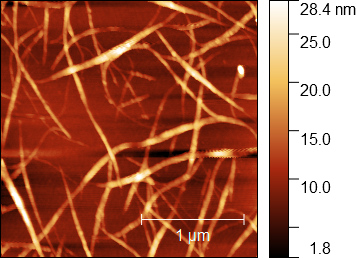
\includegraphics{./figures/ch5/Ned_NTQ24_20220125_00235.png}

}

}

\subcaption{\label{fig-bundled-network}Solvent-based deposition}
\end{minipage}%
%
\begin{minipage}[t]{0.05\linewidth}

{\centering 

~

}

\end{minipage}%
%
\begin{minipage}[t]{0.47\linewidth}

{\centering 

\raisebox{-\height}{

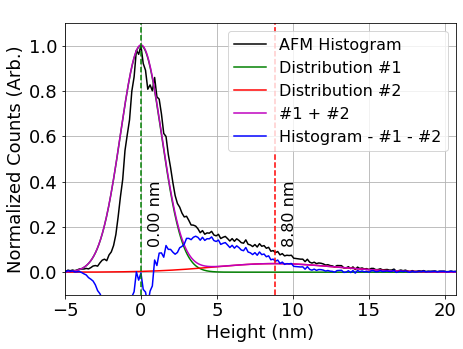
\includegraphics{./figures/ch5/Ned_NTQ24_20220125_00235_histogram_guess.png}

}

}

\subcaption{\label{fig-bundled-network-histogram}Solvent based
deposition histogram}
\end{minipage}%
\newline
\begin{minipage}[t]{0.47\linewidth}

{\centering 

\raisebox{-\height}{

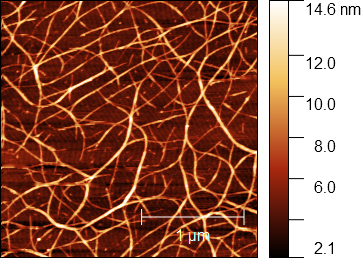
\includegraphics{./figures/ch5/Ned_NTQ8C7_w4_pristine_00084_20210428(2).png}

}

}

\subcaption{\label{fig-dropcast-network}Dropcast surfactant-based
deposition}
\end{minipage}%
%
\begin{minipage}[t]{0.05\linewidth}

{\centering 

~

}

\end{minipage}%
%
\begin{minipage}[t]{0.47\linewidth}

{\centering 

\raisebox{-\height}{

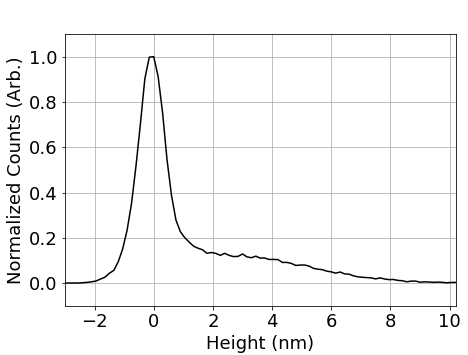
\includegraphics{./figures/ch5/Ned_NTQ8C7_w4_pristine_00084_20210428(2)_histogram_guess.png}

}

}

\subcaption{\label{fig-dropcast-network-histogram}Dropcast
surfactant-based deposition histogram}
\end{minipage}%
\newline
\begin{minipage}[t]{0.47\linewidth}

{\centering 

\raisebox{-\height}{

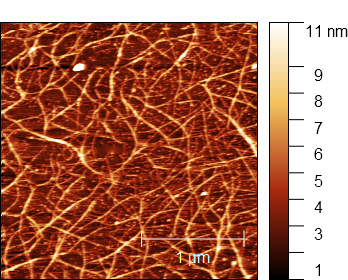
\includegraphics{./figures/ch5/Ned_NGQ14D2_W4_pristine_20220713_00567.png}

}

}

\subcaption{\label{fig-steaming-network}Steam-assisted dropcast
surfactant-based deposition}
\end{minipage}%
%
\begin{minipage}[t]{0.05\linewidth}

{\centering 

~

}

\end{minipage}%
%
\begin{minipage}[t]{0.47\linewidth}

{\centering 

\raisebox{-\height}{

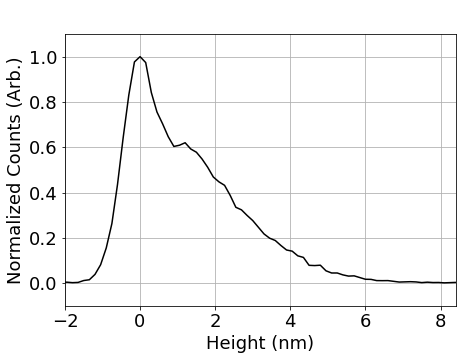
\includegraphics{./figures/ch5/Ned_NGQ14D2_W4_pristine_20220713_00567_histogram_guess.png}

}

}

\subcaption{\label{fig-steaming-network-histogram}Steam-assisted
dropcast surfactant-based deposition}
\end{minipage}%

\caption{\label{fig-afm-morphology}2.5 \(\mu\)m \(\times\) 2.5 \(\mu\)m
atomic force microscope (AFM) images of carbon nanotube films deposited
using various methods, shown side-by-side with surface profile
histograms extracted from the AFM profile. Each histogram is shown
alongside a linear combination of normal distributions \#1 and \#2,
corresponding to the silicon and carbon nanotube distribution
respectively. The counts remaining after \#1 and \#2 have been
subtracted from the AFM histogram are shown in blue.}

\end{figure}

The diameter range of deposited single-walled carbon nanotubes can be
modelled via a normal or Gaussian distribution
\autocite{LeMieux2008,Liu2013,Thanihaichelvan2018,Vobornik2023}.
However, when we extract and bin the height profiles from the 2.5
\(\mu\)m \(\times\) 2.5 \(\mu\)m AFM images, plotted in black in
Figure~\ref{fig-afm-morphology}, the histograms do not follow a normal
distribution. The reason for this result is that the carbon nanotubes do
not lie perfectly level on a perfectly level silicon oxide substrate -
the atomic force microscope histogram would only be a single normal
distribution in this ideal case. In practice, the SiO\(_2\) substrate
and carbon nanotube surface both have a degree of roughness, which may
in part be due to the presence of atmospheric contaminants. In the case
of the surfactant-deposited networks, residual surfactant may also
contribute to surface roughness \autocite{Vobornik2023}. Furthermore,
nanotubes overlap and cross over each other, creating junctions with the
combined height of the overlapping nanotubes.

It has been demonstrated that the surface roughness of a bare SiO\(_2\)
substrate can also be modelled with a normal distribution. This normal
distribution can be set as the reference or zero point for other height
measurements \autocite{Velicky2015}. As both the carbon nanotube and
silicon dioxide background heights can each be modelled using a normal
distribution, we make an initial assumption that a linear combination of
normal distributions can be used to model the AFM histograms in
Figure~\ref{fig-afm-morphology}. Using the process discussed in
Section~\ref{sec-histogram-analysis}, we approximate the normal
distributions corresponding to the silicon oxide substrate and carbon
nanotube network, shown in Figure~\ref{fig-afm-morphology} as green and
red curves respectively. The silicon oxide peak appears to fit more
closely to the distribution with smaller carbon nanotube heights, which
could be due to measurement of the silicon background being improved
when feature height is smaller. We notice that the distribution for the
carbon nanotube bundles drops to approximately zero before reaching 0
nm, which is physically appropriate.

\begin{figure}

\begin{minipage}[t]{0.47\linewidth}

{\centering 

\raisebox{-\height}{

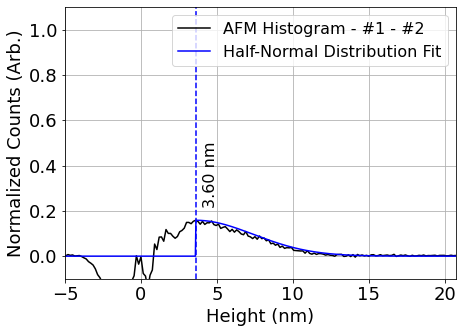
\includegraphics{./figures/ch5/Ned_NTQ24_20220125_00235_half_histogram_fit.png}

}

}

\subcaption{\label{fig-bundled-network-remainder}Solvent based
deposition histogram}
\end{minipage}%
%
\begin{minipage}[t]{0.05\linewidth}

{\centering 

~

}

\end{minipage}%
%
\begin{minipage}[t]{0.47\linewidth}

{\centering 

\raisebox{-\height}{

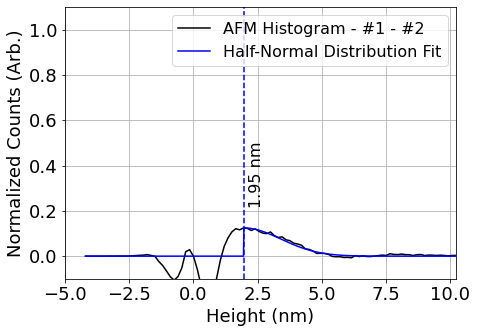
\includegraphics{./figures/ch5/Ned_NTQ8C7_w4_pristine_00084_20210428(2)_half_histogram_fit.png}

}

}

\subcaption{\label{fig-dropcast-network-remainder}Dropcast
surfactant-based deposition histogram}
\end{minipage}%
\newline
\begin{minipage}[t]{0.26\linewidth}

{\centering 

~

}

\end{minipage}%
%
\begin{minipage}[t]{0.47\linewidth}

{\centering 

\raisebox{-\height}{

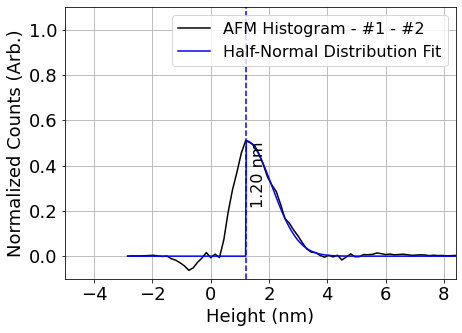
\includegraphics{./figures/ch5/Ned_NGQ14D2_W4_pristine_20220713_00567_half_histogram_fit.png}

}

}

\subcaption{\label{fig-steaming-network-remainder}Steam-assisted
dropcast surfactant-based deposition}
\end{minipage}%
%
\begin{minipage}[t]{0.26\linewidth}

{\centering 

~

}

\end{minipage}%

\caption{\label{fig-remaining-histogram}The counts which remain after
\#1 and \#2 have been subtracted from the AFM histogram are shown in
black. The counts have been overlaid with half a Gaussian distribution,
manually fitted.}

\end{figure}

By subtracting the modelled silicon and carbon nanotube normal
distributions from the AFM histogram, we find a remaining distribution
spread roughly between 0 nm and the mean of the carbon nanotube bundle
distribution. Interestingly, the peak of the carbon nanotube
distribution occurs at a height approximately 2.5\(\times\) the height
corresponding to the peak of the remaining distribution. It is also
apparent that the remaining distribution consistently follows a normal
distribution after a sharp rise to maximum, as shown in
Figure~\ref{fig-remaining-histogram}. This distribution appears to
correspond to surface roughness due to the presence of contaminants, or
possibly to broken pieces of individual nanotubes with various lengths.
Contaminants could be residual surfactant or other atmospheric
contamination resistant to acetone and isopropanol rinsing. Such
contamination may or may not have implications for biosensing
suitability, but surfactant contamination could certainly have negative
effects on biological elements sensitive to surfactant. The area of this
central peak may be useful for determining the extent of contamination
on a carbon nanotube film, discussed further in
\textbf{?@sec-contamination}.

If we model carbon nanotube bundles as cylinders, and we assume the
component nanotubes follow 2D packing and are of equal diameter, we can
give an estimate the mean bundle size for each deposition type in terms
of number of nanotubes \emph{n}
\autocite{Graham1998,Thanihaichelvan2018,Specht2023}.

\hypertarget{tbl-circle-packing}{}
\begin{longtable}[]{@{}
  >{\raggedright\arraybackslash}p{(\columnwidth - 16\tabcolsep) * \real{0.1053}}
  >{\raggedright\arraybackslash}p{(\columnwidth - 16\tabcolsep) * \real{0.1228}}
  >{\raggedright\arraybackslash}p{(\columnwidth - 16\tabcolsep) * \real{0.0965}}
  >{\raggedright\arraybackslash}p{(\columnwidth - 16\tabcolsep) * \real{0.0965}}
  >{\raggedright\arraybackslash}p{(\columnwidth - 16\tabcolsep) * \real{0.1228}}
  >{\raggedright\arraybackslash}p{(\columnwidth - 16\tabcolsep) * \real{0.1228}}
  >{\raggedright\arraybackslash}p{(\columnwidth - 16\tabcolsep) * \real{0.1228}}
  >{\raggedright\arraybackslash}p{(\columnwidth - 16\tabcolsep) * \real{0.1228}}
  >{\raggedright\arraybackslash}p{(\columnwidth - 16\tabcolsep) * \real{0.0877}}@{}}
\caption{\label{tbl-circle-packing}The first eight optimised ratios of
2D packed circle diameter to encompassing circle diameter, given to 3
s.f. (encompassing circle diameter = \(d\), number of packed circles =
\(n\), approximate packed circle diameter = \(d_n\)).\\
}\tabularnewline
\toprule()
\endhead
\(n\) & \text{2} & \text{3} & \text{4} & \text{5} & \text{6} & \text{7}
& \text{8} & \text{9} \\
\(d\)/\(d_n\) & \text{2.00} & 2.15 & 2.41 & \text{2.70} & \text{3.00} &
\text{3.00} & \text{3.30} & 3.61 \\
\bottomrule()
\end{longtable}

Table~\ref{tbl-circle-packing} shows the relationship between the
diameter of a bundle and the constituent diameters of up to nine 2D
packed carbon nanotubes within that bundle. Assuming an average carbon
nanotube diameter of 1.45 nm, we can use the \(d\)/\(d_n\) packing
ratios to obtain an estimate of the number of nanotubes in the mean
bundle size for each deposition \autocite{Specht2023}. We can also give
an approximate range which this estimate falls within using the provided
range of individual carbon nanotube diameters (\(1.2-1.7\) nm) and the
95\% confidence interval of the mean bundle size (\(2\sigma\)). These
estimates are shown in Table~\ref{tbl-histogram-parameters}. Also shown
is an estimate of the ratio of single- to multi-tube bundles for each
deposition, found by comparing the proportion of each carbon nanotube
curve below and above 2.9 nm, the minimum multi-tube bundle size for
1.45 nm diameter nanotubes. It should be noted that the force of the
atomic force microscope tip may cause some degree of nanotube bundle
compression, leading to a systematic underestimate of nanotube height
\autocite{Vobornik2023}. The relative proportion of multi-tube bundles
shown in Table~\ref{tbl-histogram-parameters} should therefore be
treated as a lower-limit estimate of the true proportion.

\hypertarget{tbl-histogram-parameters}{}
\begin{table}
\caption{\label{tbl-histogram-parameters}The mean of histogram distributions for carbon nanotube films deposited
using various methods, alongside estimates for the number of nanotubes
present per bundle (within a 95\% confidence interval) and the
proportion of multi-tubed bundles present across the network. The value
in brackets corresponds to an estimate for the number of nanotubes
present in the mean bundle size. }\tabularnewline

\centering
\begin{tabular}{>{\raggedright\arraybackslash}p{2cm}ccccc}
\toprule
\multicolumn{1}{c}{\textbf{ }} & \multicolumn{3}{c}{\textbf{Distribution Mean (nm)}} & \multicolumn{2}{c}{\textbf{Bundle Attributes}} \\
\cmidrule(l{3pt}r{3pt}){2-4} \cmidrule(l{3pt}r{3pt}){5-6}
 & Silicon & Bundles & Contaminant & Tubes/Bundle & \% Multi-Tube\\
\midrule
Solvent deposited & 0.0 ± 1.4 & 8.8 ± 4.0 & 3.6 ± 3.8 & 1–162 (28) & \textasciitilde{}95\%\\
 &  &  &  &  \vphantom{1} & \\
Surfactant deposited & 0.0 ± 0.6 & 5.1 ± 1.4 & 2.0 ± 1.5 & 2–34 (8) & \textasciitilde{}94\%\\
 &  &  &  &  & \\
Surfactant deposited with steam & 0.0 ± 0.5 & 3.2 ± 1.1 & 1.2 ± 0.9 & 1–15 (3) & \textasciitilde{}60\%\\
\bottomrule
\end{tabular}
\end{table}

When surfactant is used in the deposition process, both the carbon
nanotube bundle diameter mean and standard deviation are small compared
to the mean and standard deviation of solvent deposited films. However,
despite the presence of surfactant, it is apparent both from
Figure~\ref{fig-afm-morphology} and Table~\ref{tbl-histogram-parameters}
that not all surfactant-dispersed carbon nanotubes are deposited
individually. Bundling may occur during the process of deposition onto
the substrate, which could disrupt the repulsive forces from the
surfactant coating and allow attractive forces to temporarily dominate.

It is possible that the bundling of surfactant-dispersed carbon
nanotubes is a consequence of dynamics introduced by the coffee-ring
effect \autocite{Deegan1997,VanGaalen2021}. The coffee-ring effect
refers to a build-up of dispersed solid forming around the edges of a
dispersion evaporating on a surface. This process occurs due to the
dispersion edges being fixed by surface forces, leading to capillary
flow outwards to replace liquid evaporating at the edges, bringing solid
material along with it. The presence of vapour is known to disrupt this
capillary effect \autocite{Bishop2020}.

\hypertarget{sec-pristine-electrical-characterisation}{%
\section{Electrical
Characteristics}\label{sec-pristine-electrical-characterisation}}

\hypertarget{carbon-nanotubes}{%
\subsection{Carbon Nanotubes}\label{carbon-nanotubes}}

\begin{figure}

\begin{minipage}[t]{0.49\linewidth}

{\centering 

\raisebox{-\height}{

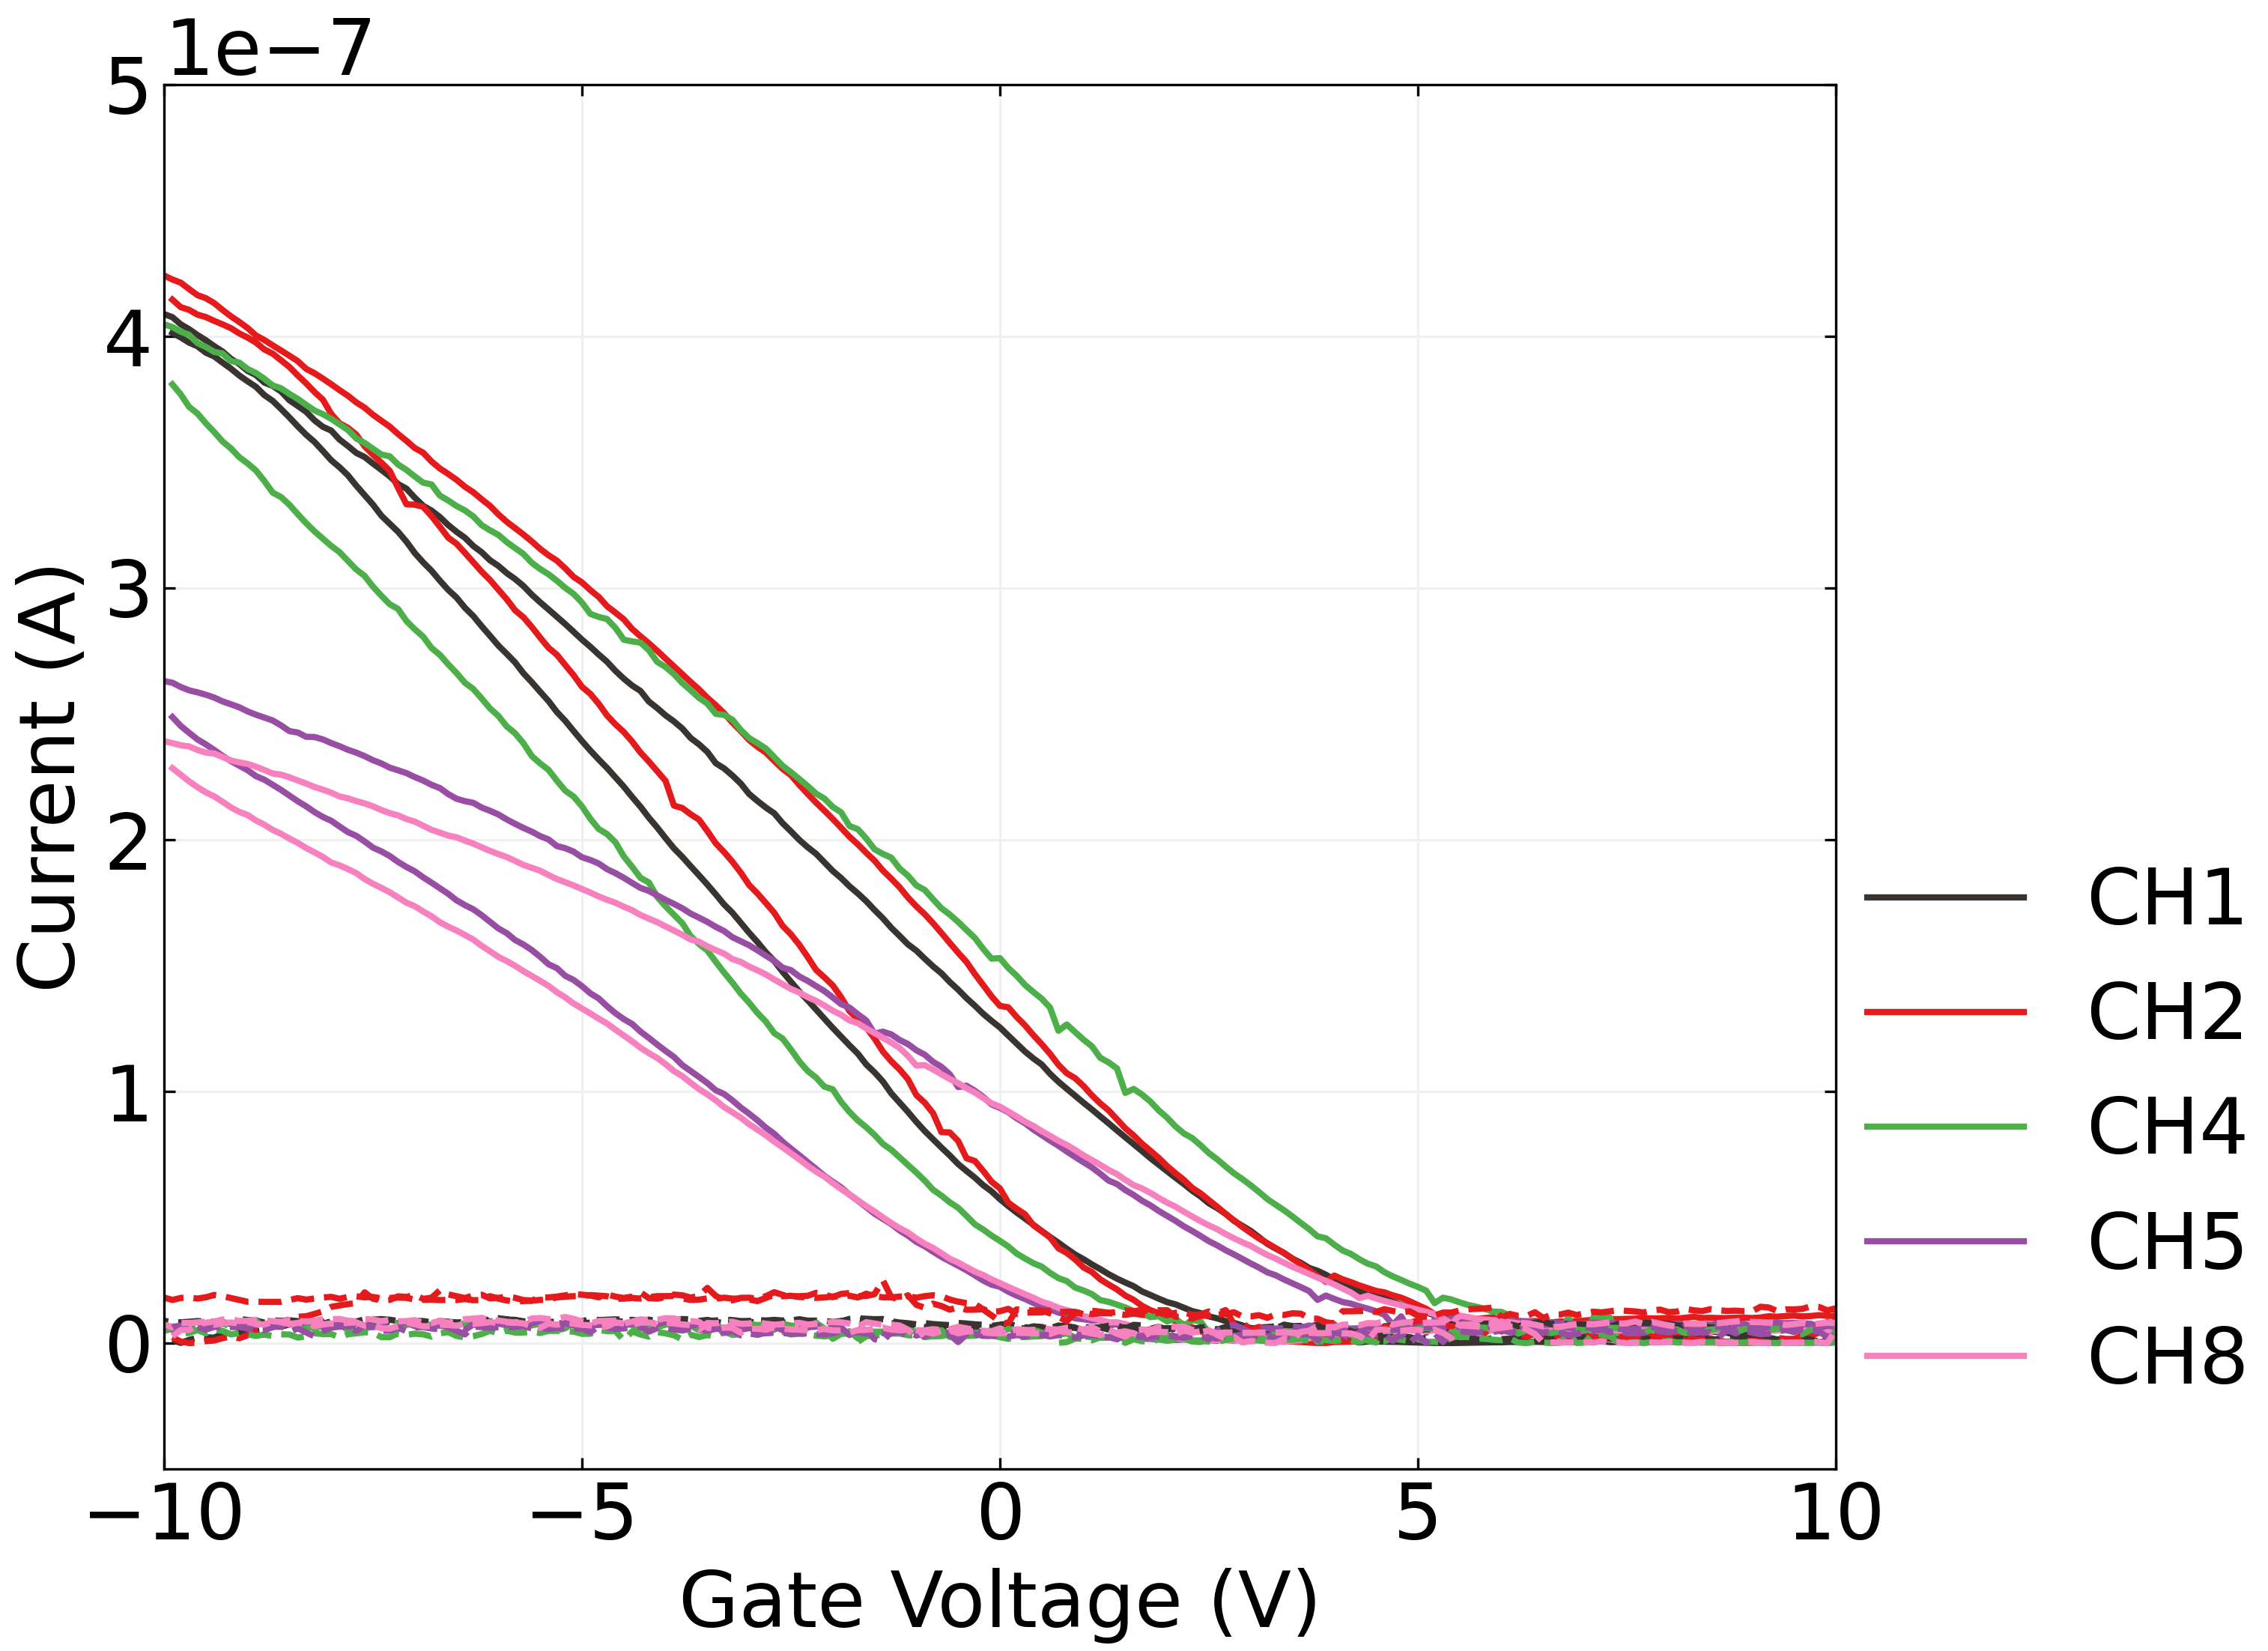
\includegraphics{./figures/ch5/NTQ22C2_solvent_backgate.png}

}

}

\subcaption{\label{fig-solvent-tx-bg}Solvent-based deposition,
back-gated}
\end{minipage}%
%
\begin{minipage}[t]{0.02\linewidth}

{\centering 

~

}

\end{minipage}%
%
\begin{minipage}[t]{0.49\linewidth}

{\centering 

\raisebox{-\height}{

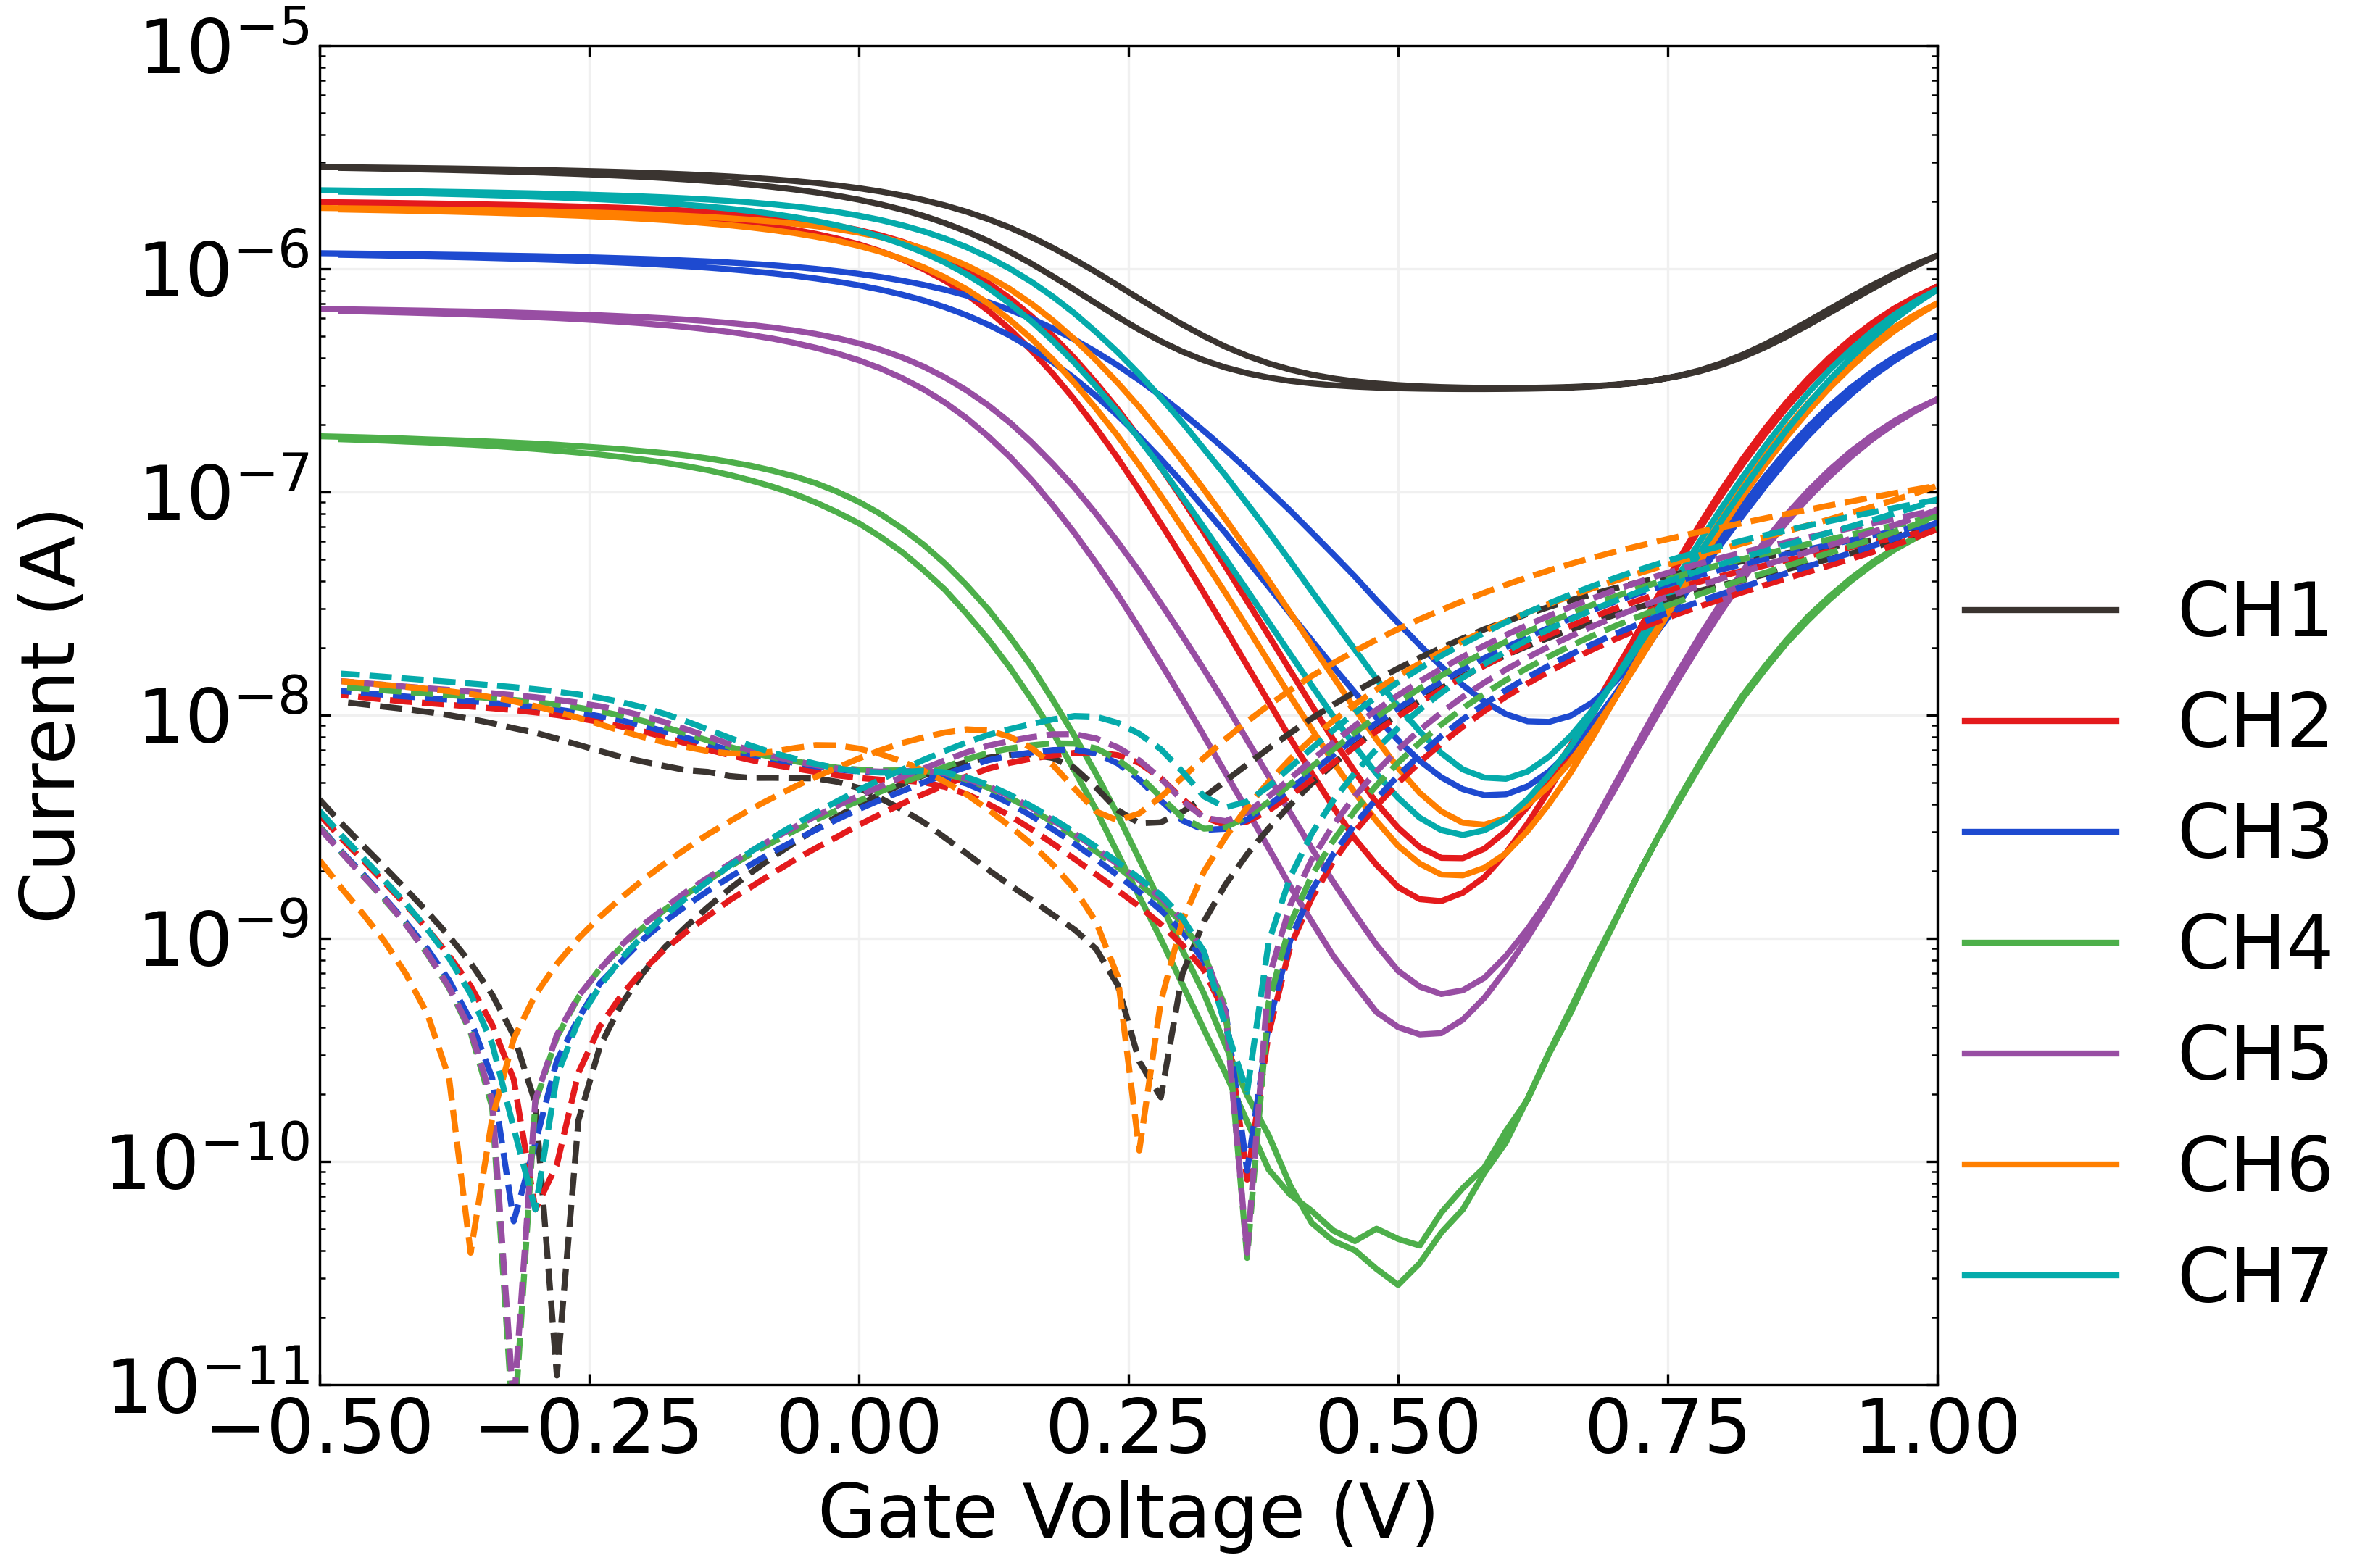
\includegraphics{./figures/ch5/NTQ24C8_pristine_TXLG01_220211_solvent_gate.png}

}

}

\subcaption{\label{fig-solvent-tx-lg}Solvent-based deposition,
liquid-gated}
\end{minipage}%
\newline
\begin{minipage}[t]{0.49\linewidth}

{\centering 

\raisebox{-\height}{

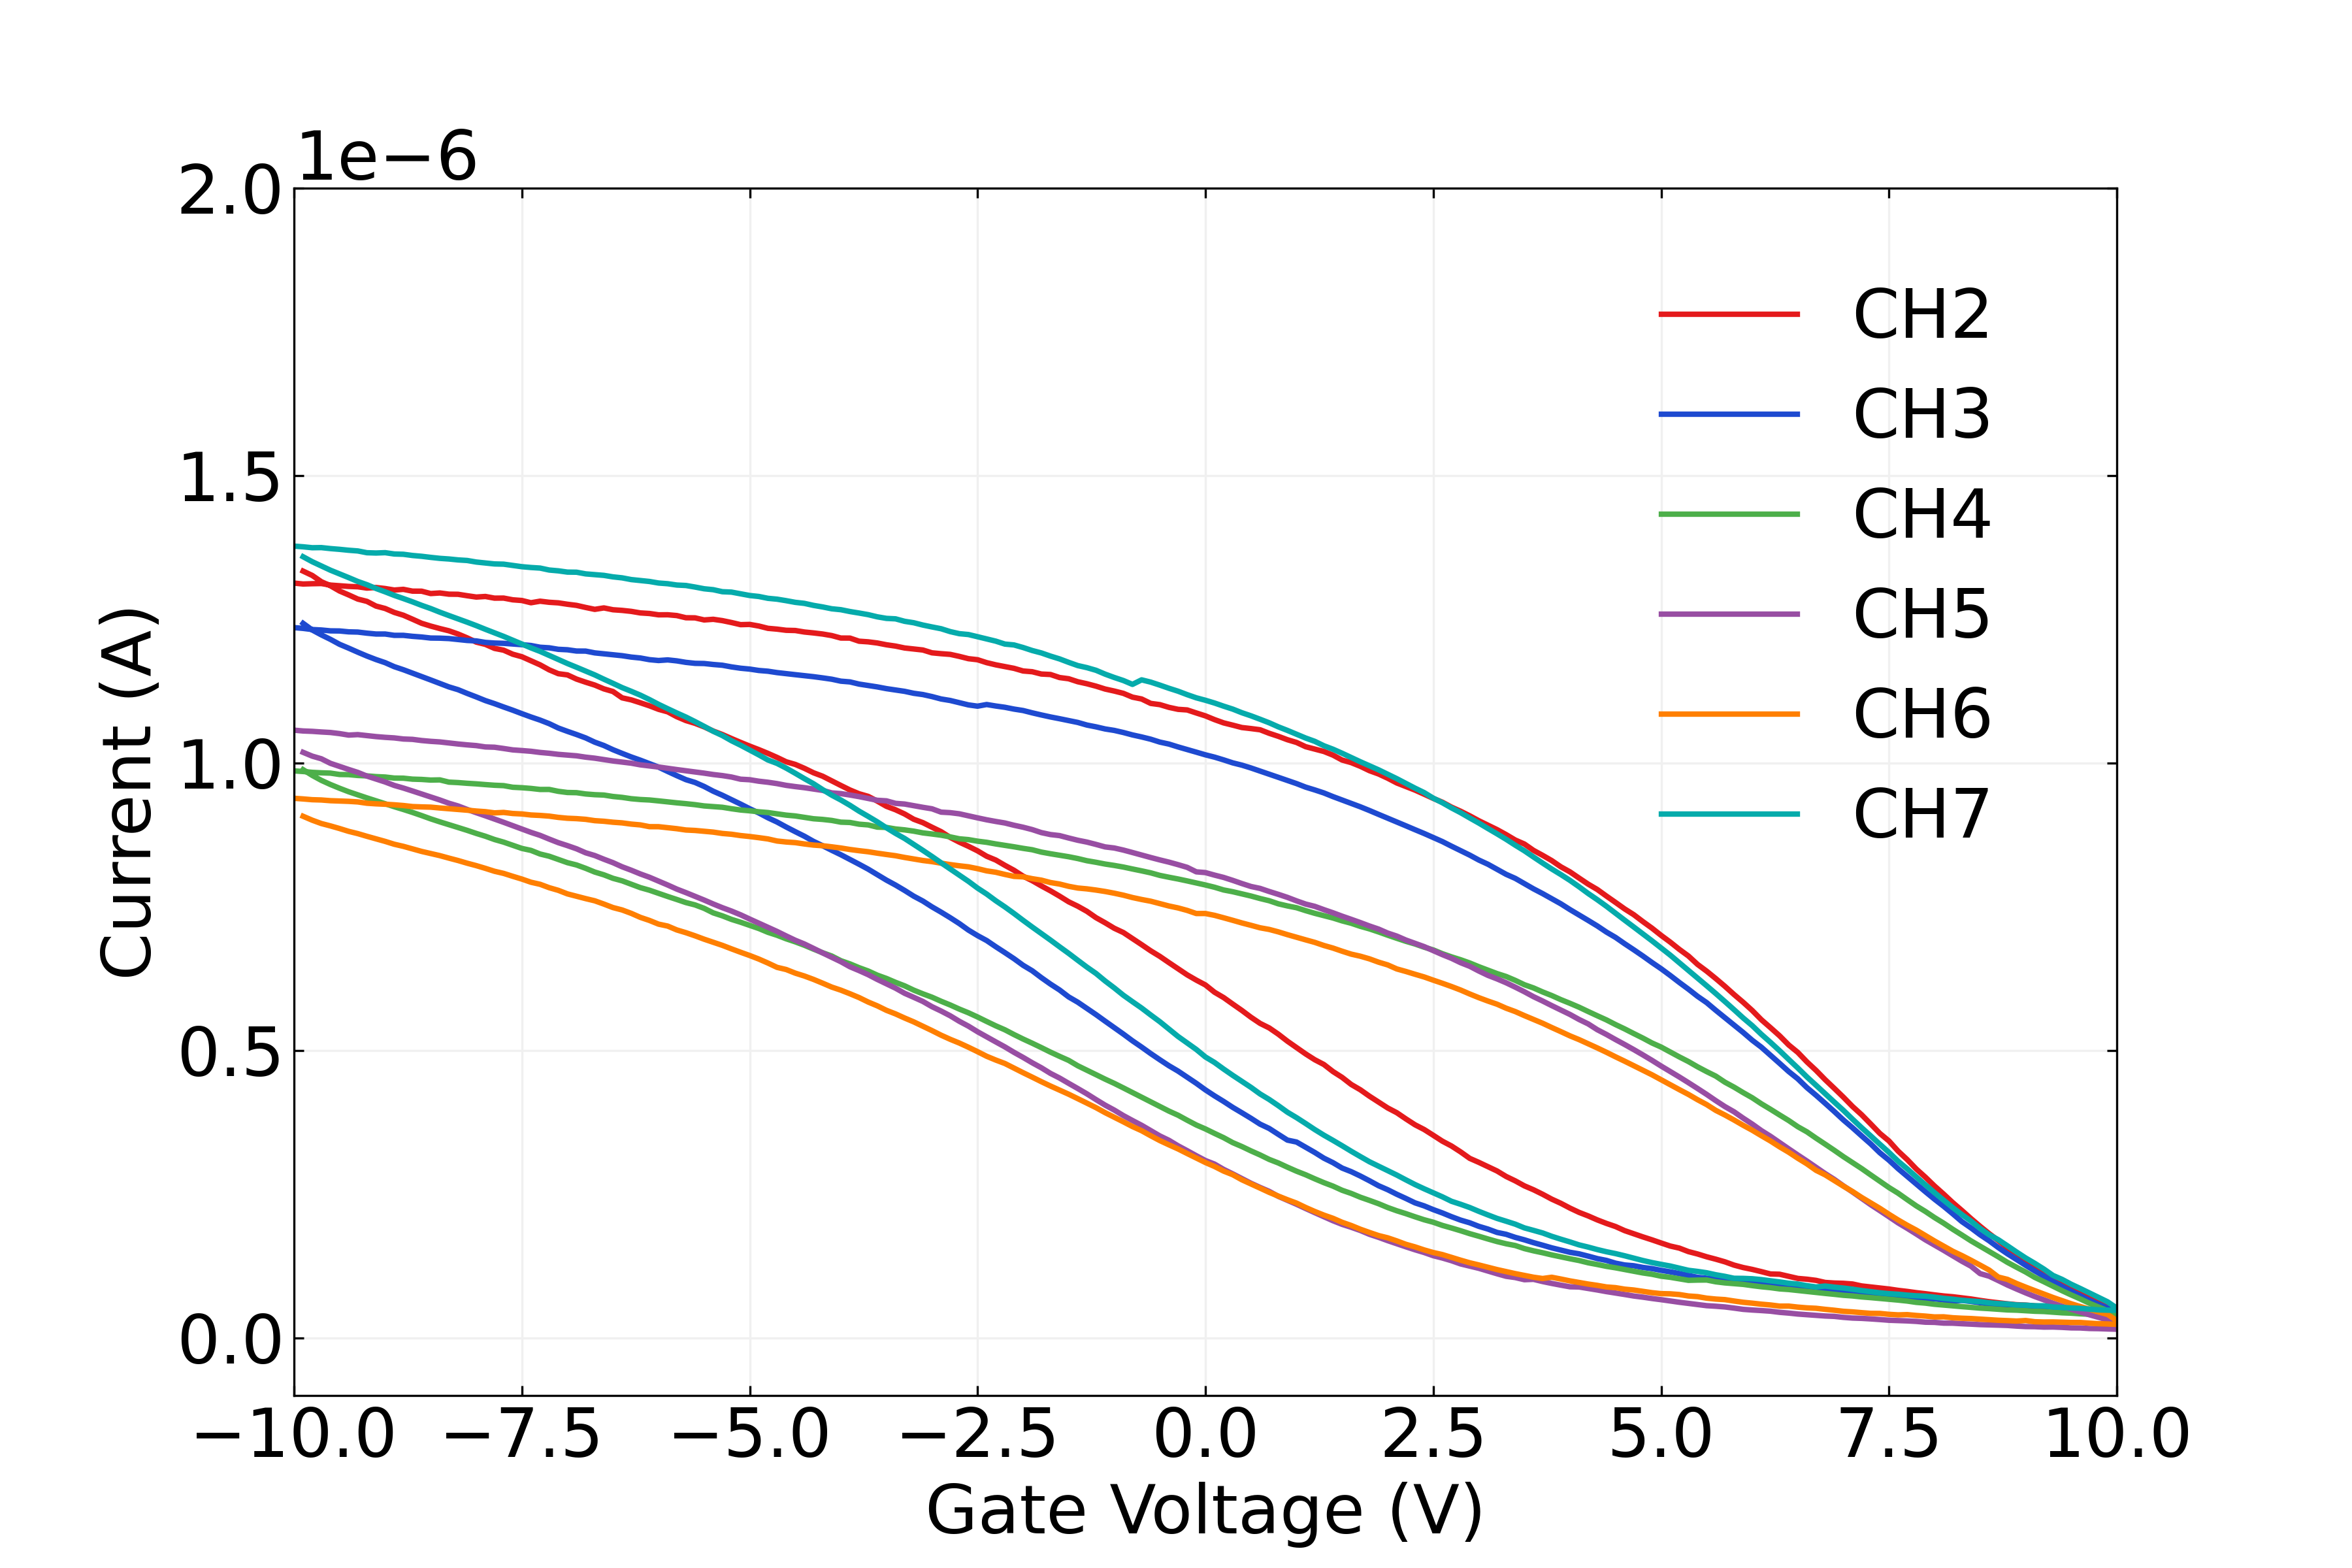
\includegraphics{./figures/ch5/Q5C10_nosteam_backgate.png}

}

}

\subcaption{\label{fig-surf-tx-bg}Dropcast surfactant-based deposition,
back-gated}
\end{minipage}%
%
\begin{minipage}[t]{0.02\linewidth}

{\centering 

~

}

\end{minipage}%
%
\begin{minipage}[t]{0.49\linewidth}

{\centering 

\raisebox{-\height}{

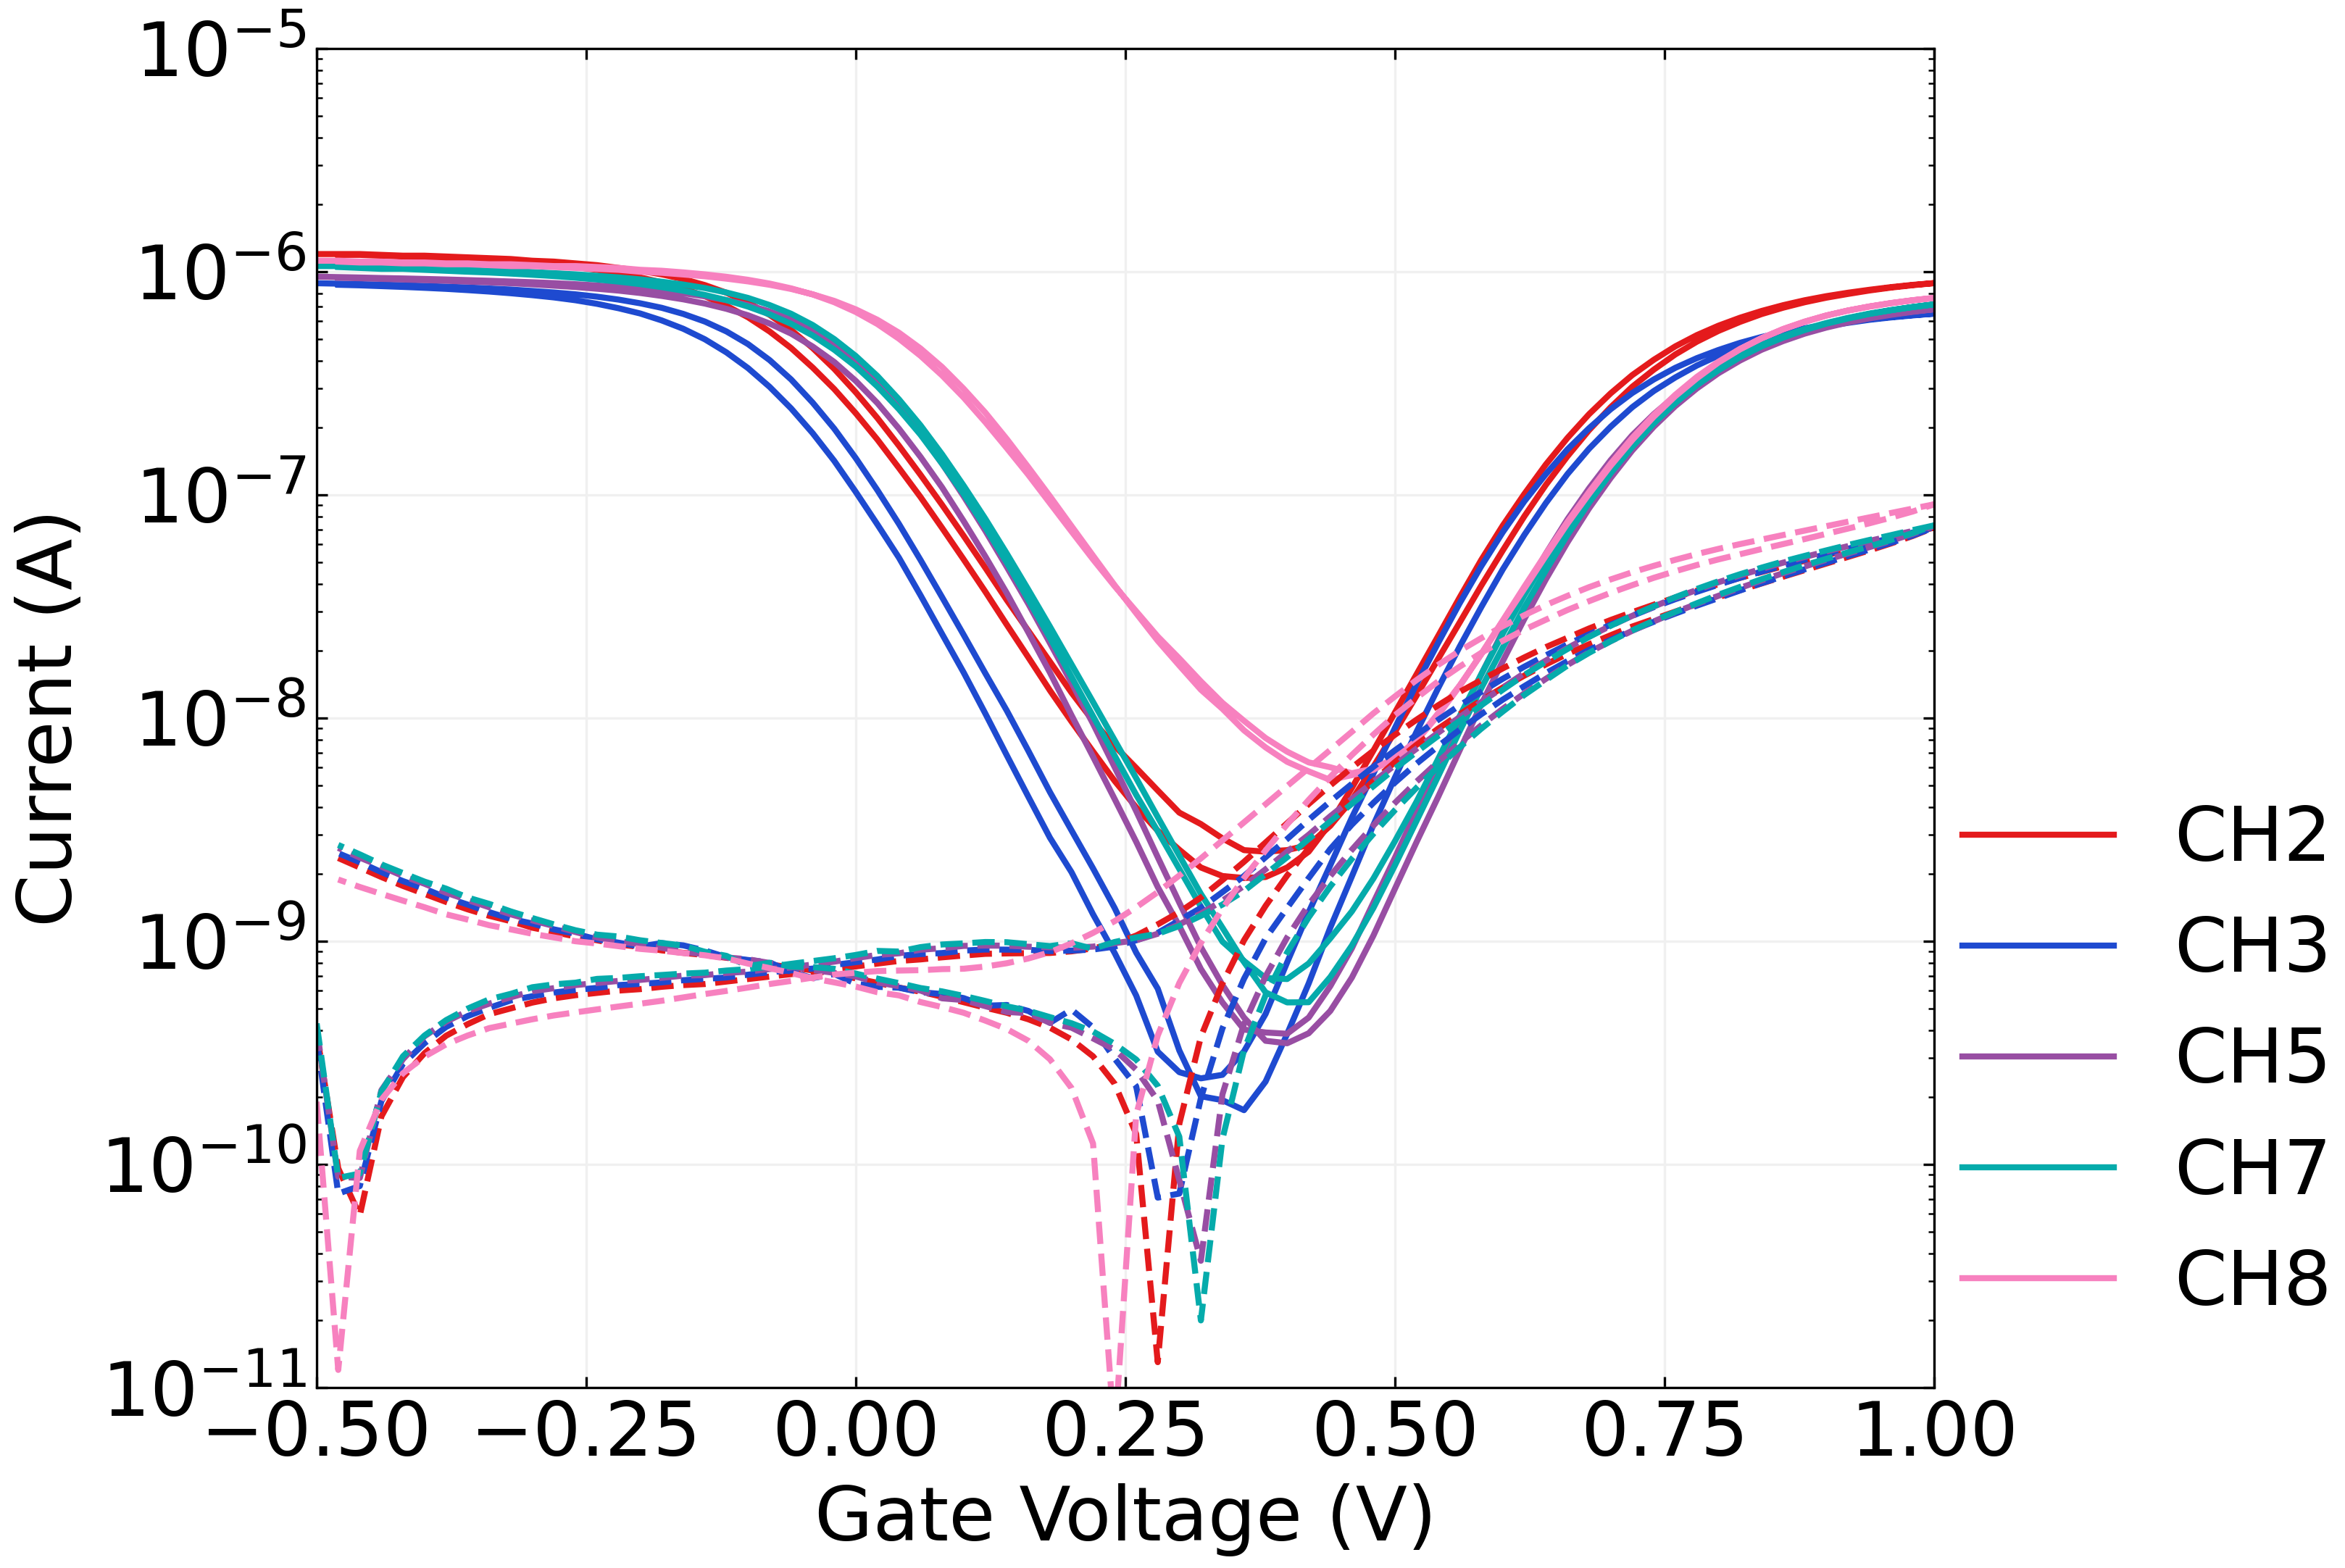
\includegraphics{./figures/ch5/NTQ5C3_pristine_TXLG01_210602_nosteam_gate.png}

}

}

\subcaption{\label{fig-surf-tx-lg}Dropcast surfactant-based deposition,
liquid-gated}
\end{minipage}%
\newline
\begin{minipage}[t]{0.49\linewidth}

{\centering 

\raisebox{-\height}{

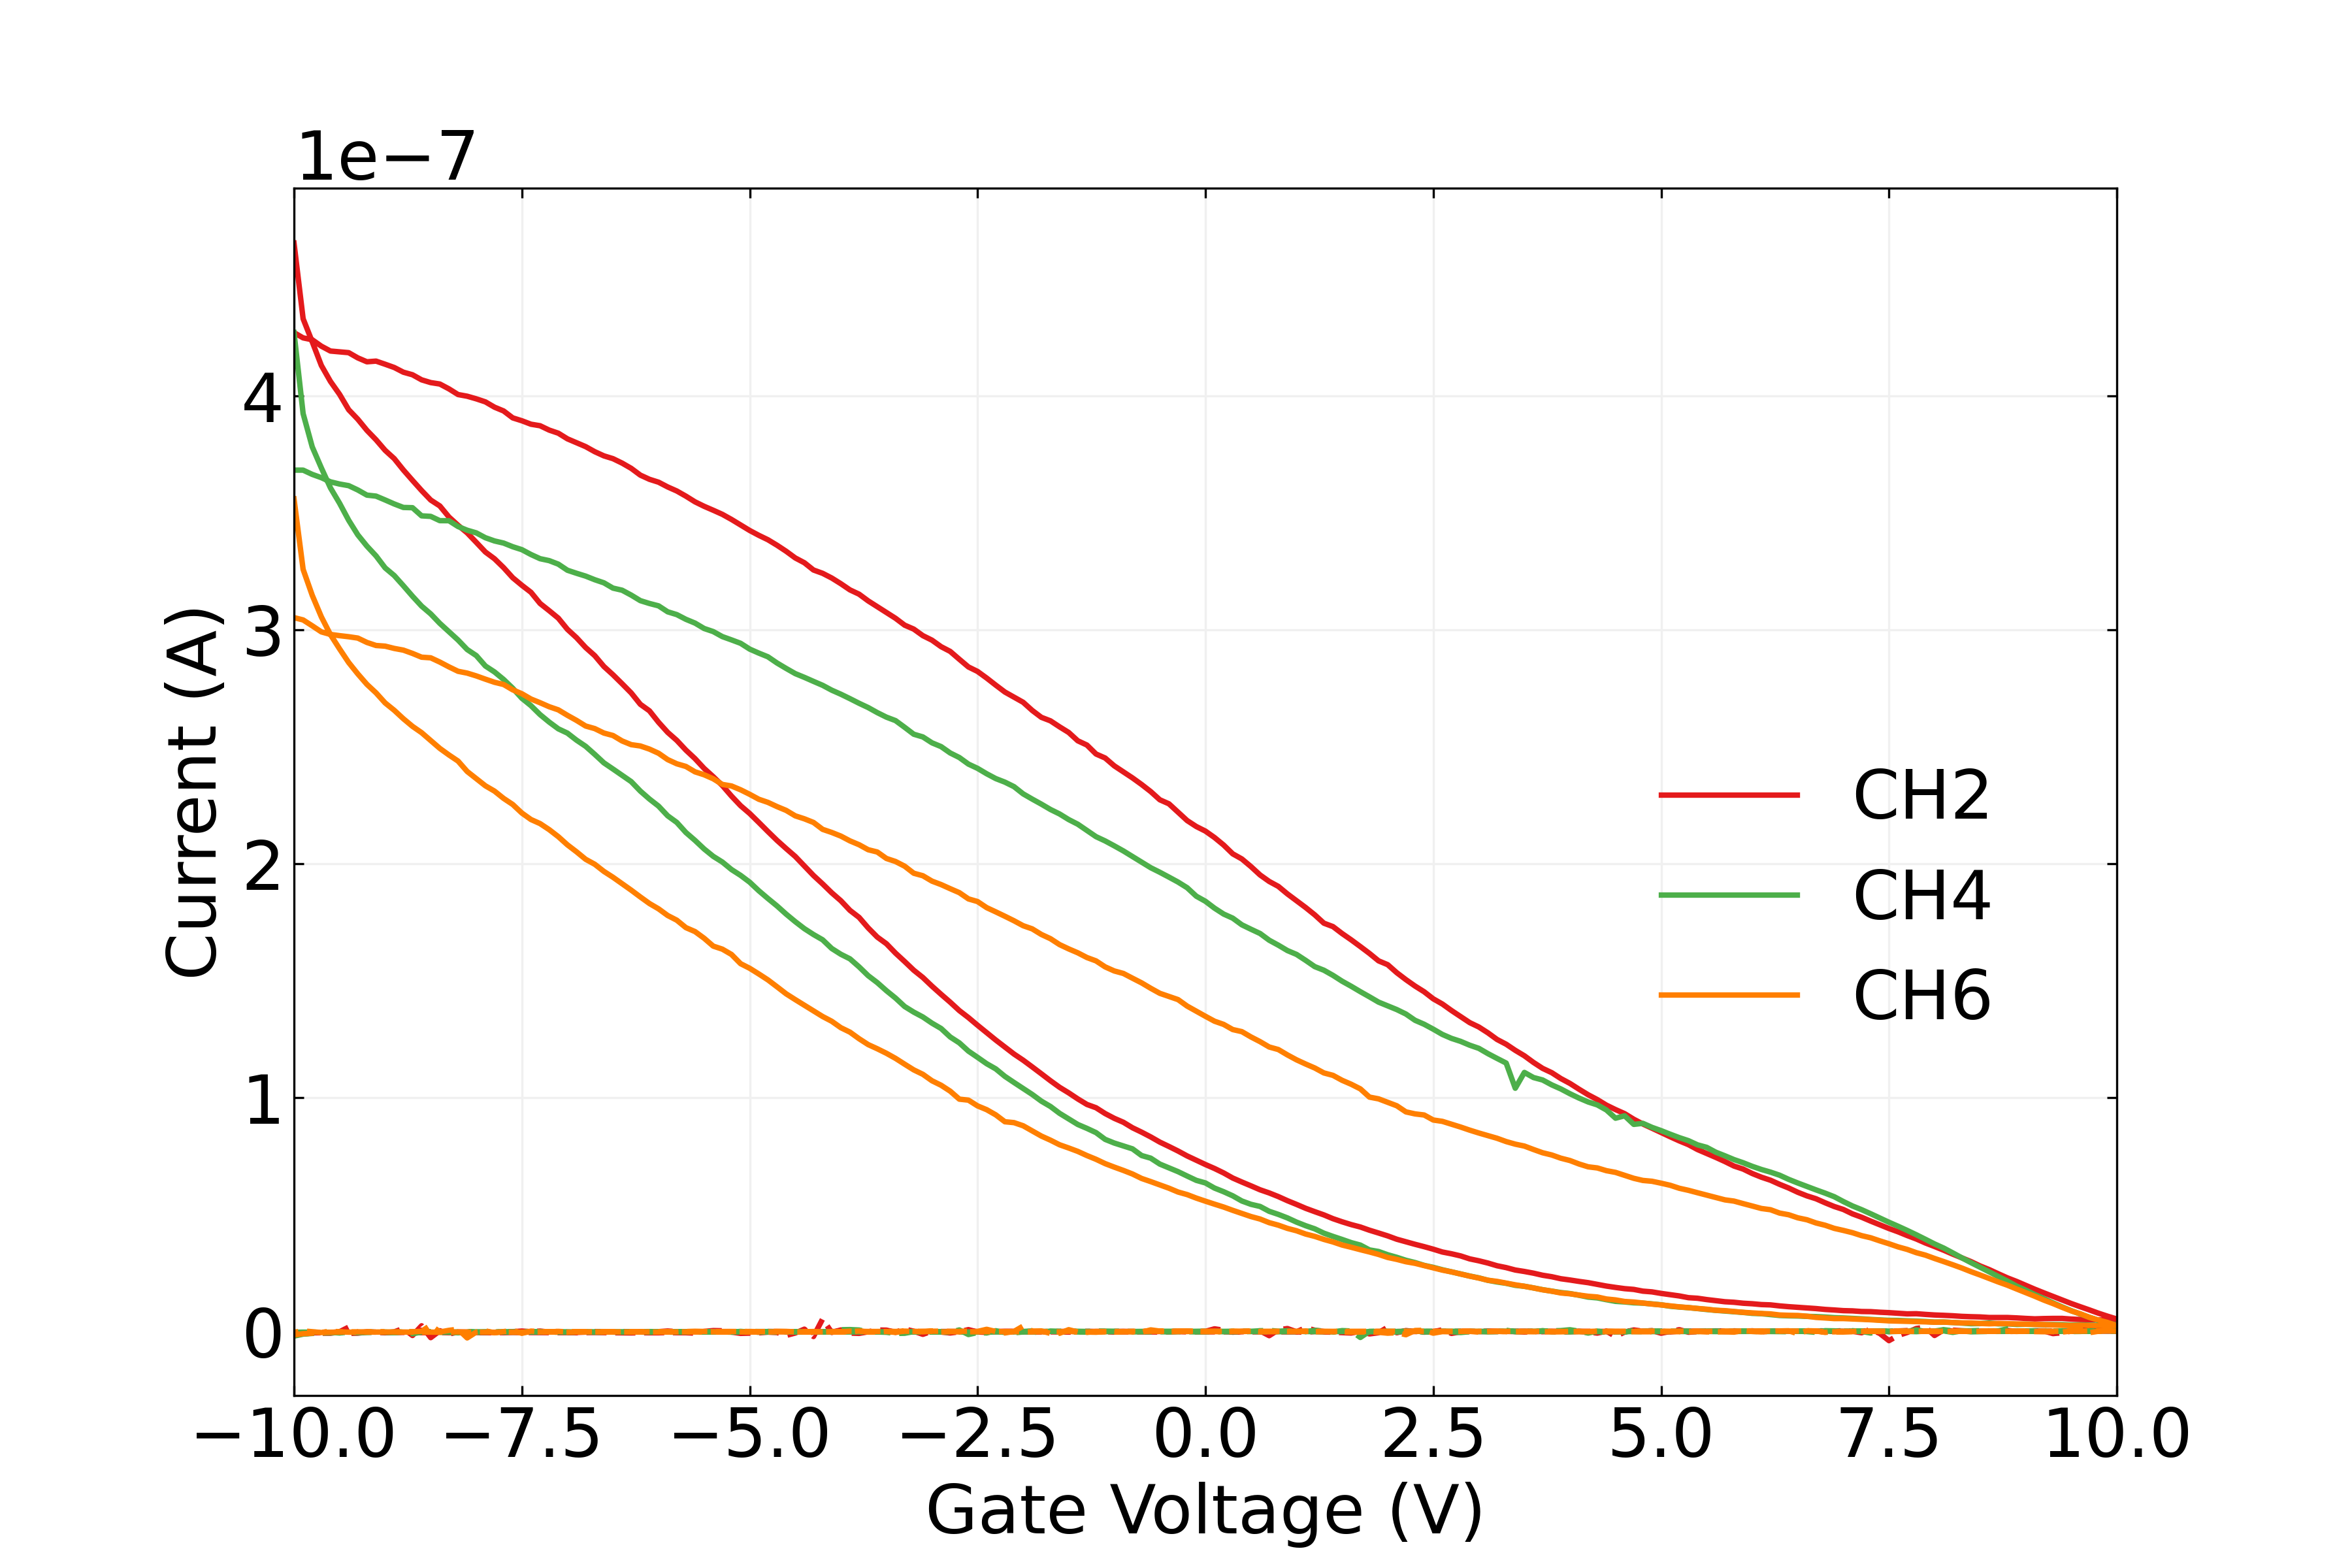
\includegraphics{./figures/ch5/Q18C6_steam_backgate.png}

}

}

\subcaption{\label{fig-steam-tx-bg}Steam-assisted dropcast
surfactant-based deposition, back-gated}
\end{minipage}%
%
\begin{minipage}[t]{0.02\linewidth}

{\centering 

~

}

\end{minipage}%
%
\begin{minipage}[t]{0.49\linewidth}

{\centering 

\raisebox{-\height}{

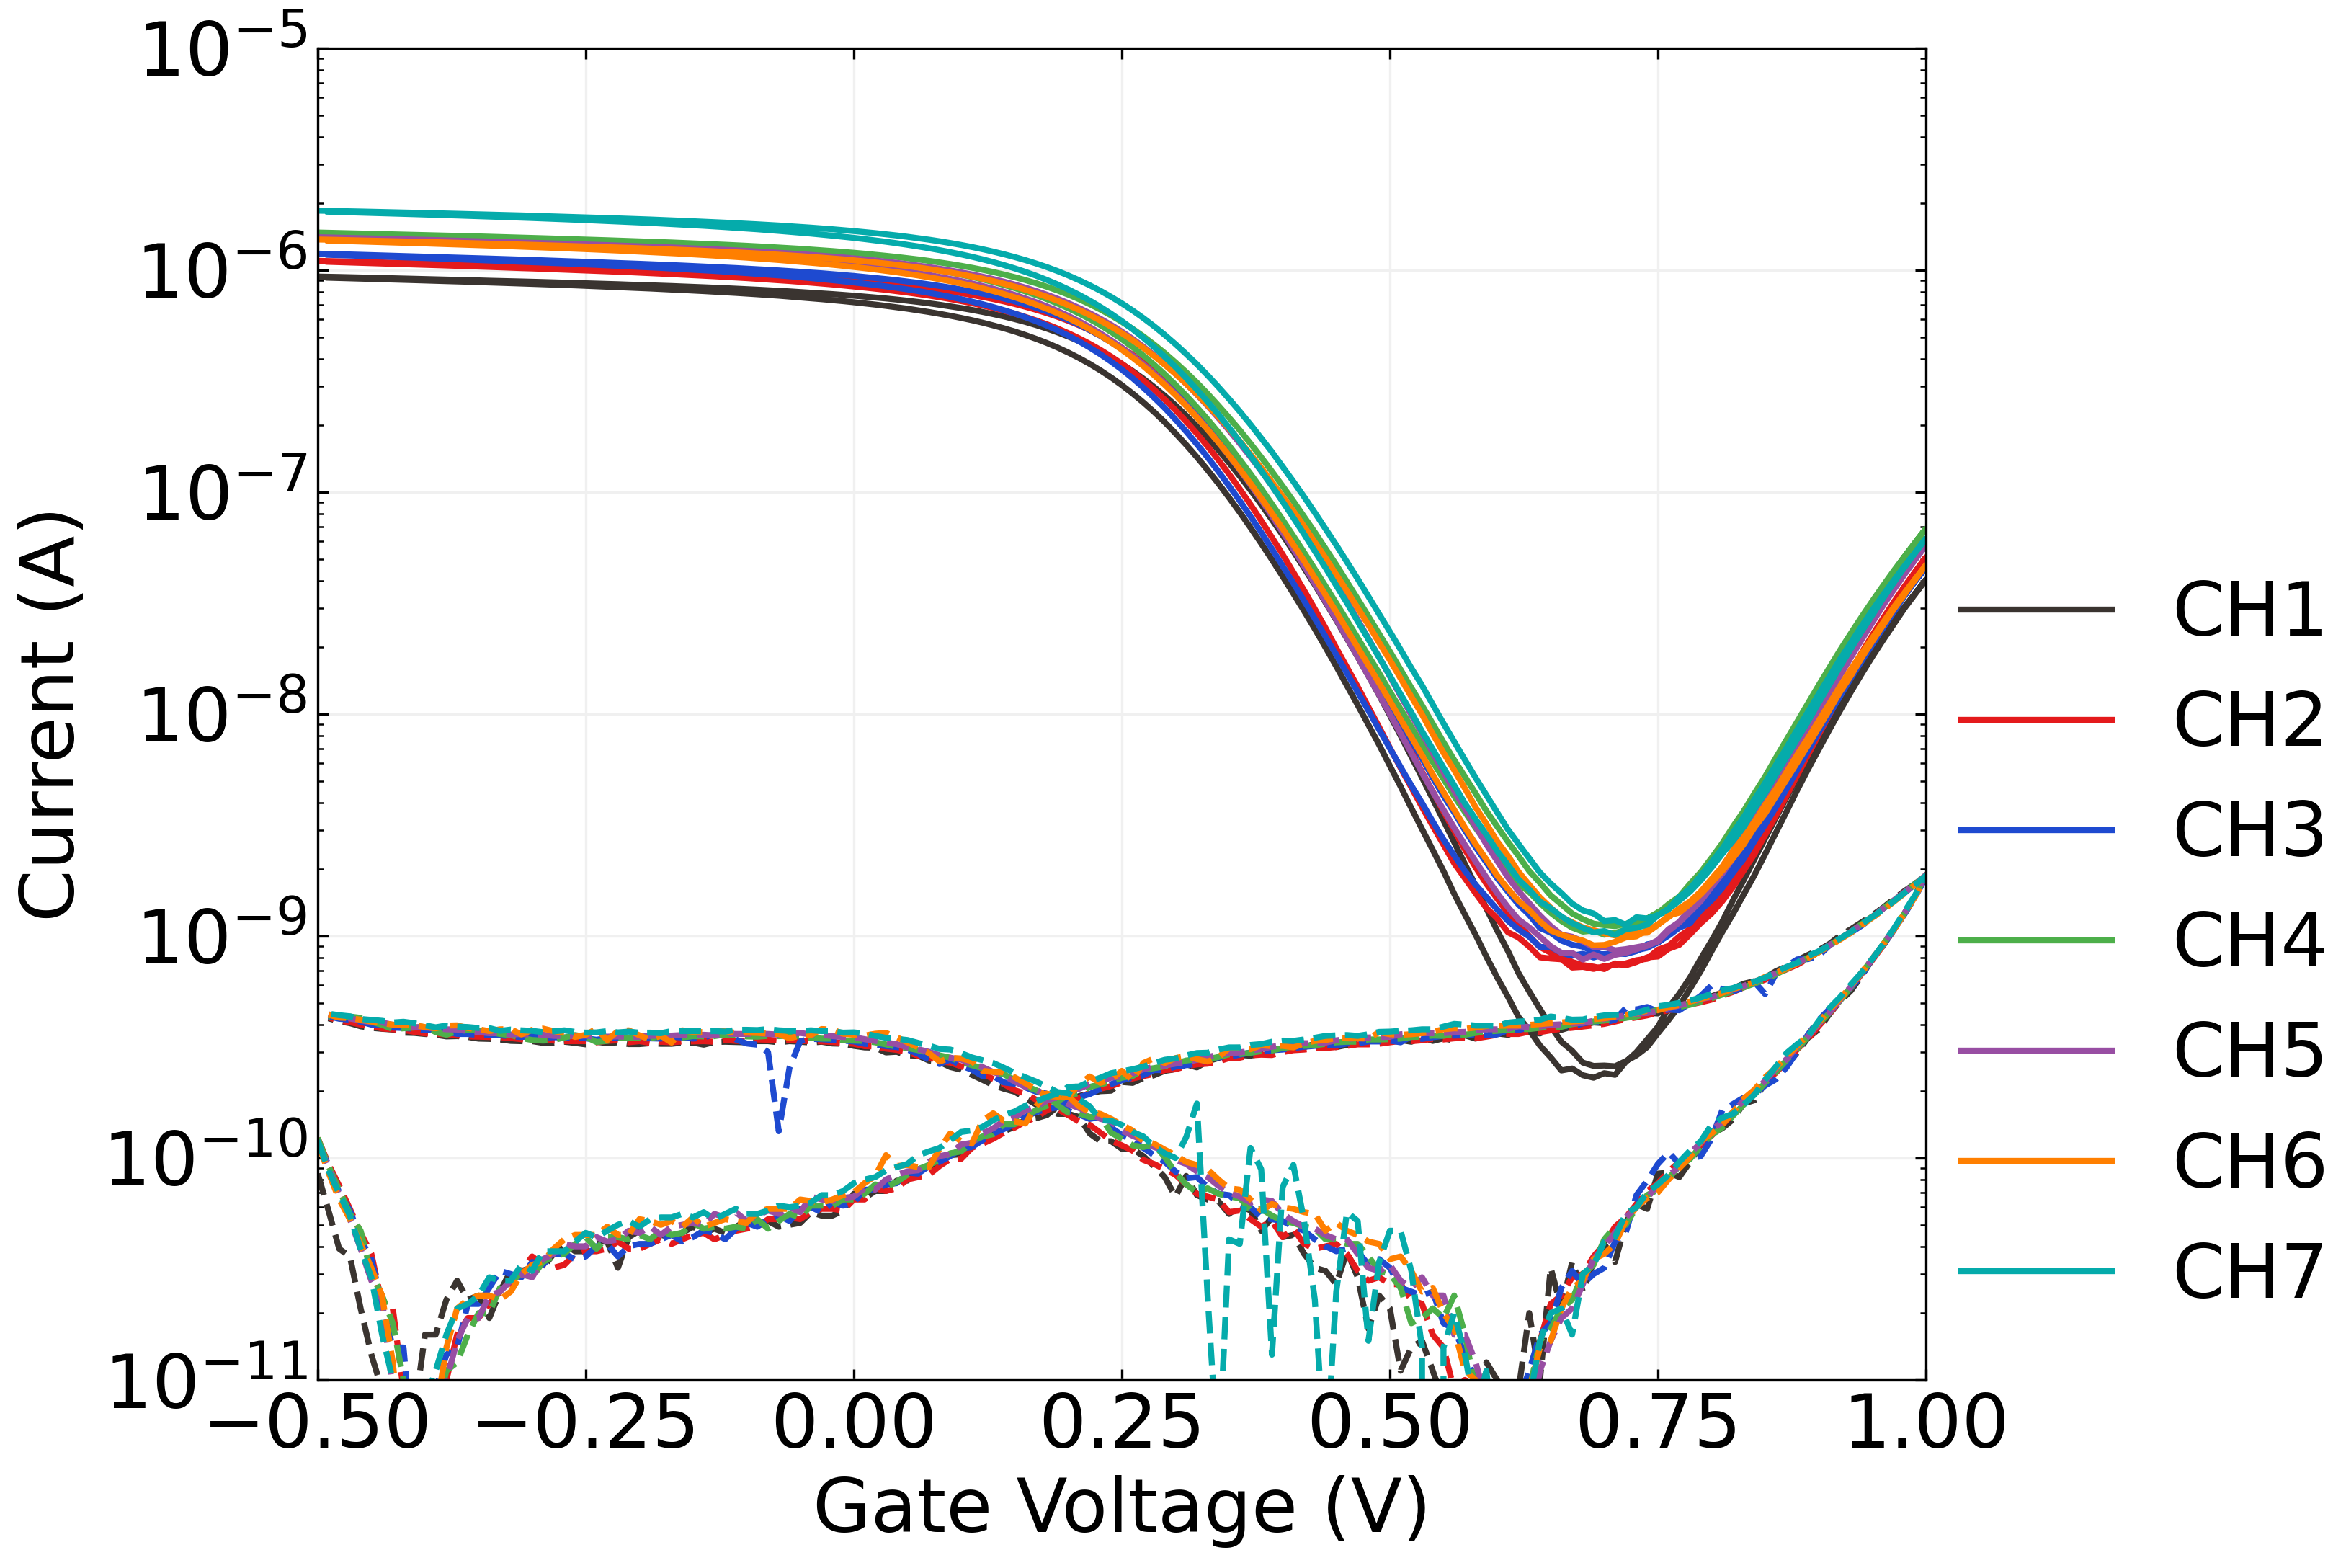
\includegraphics{./figures/ch5/NTQ31C6_pristine_TXLG01_230330_steam_gate.png}

}

}

\subcaption{\label{fig-steam-tx-lg}Steam-assisted dropcast
surfactant-based deposition, liquid-gated}
\end{minipage}%

\caption{\label{fig-pristine-cnt-characteristics}Transfer
characteristics of AZ\(^\circledR\) 1518 encapsulated field-effect
transistors with carbon nanotube network channels deposited using
various methods. 1XPBS was used as the buffer for the liquid-gated
measurements here. The source-drain voltage used for all sweeps was
\(V_{ds} = 100 \textrm{mV}\). A step size of 20 mV was used for the
liquid-gated sweeps, while a step size of 100 mV was used for the
backgated sweeps. Each pair of sweeps was taken from a separate device.
Devices with a 100 nm SiO\(_2\) layer were used for backgated
measurements, and devices with a 300 nm SiO\(_2\) layer were used for
liquid gated measurements.}

\end{figure}

Each carbon nanotube device fabricated was electrically characterised as
described in \textbf{?@sec-electrical-characterisation}, and electrical
data was analysed using the Python code discussed in
Section~\ref{sec-field-effect-transistor-analysis}.

Figure~\ref{fig-pristine-cnt-characteristics} displays multi-channel
measurements of representative devices fabricated as described in
\textbf{?@sec-fabrication}. To ensure a consistent comparison, each
device here was encapsulated with AZ\(^\circledR\) 1518 encapsulation
before measurements were taken. The channels which did not exhibit
reliable transistor characteristics are not shown. These `non-working'
channels were either shorted, due to metal remaining on the channel
after lift-off, or were very low current, due to a very sparse carbon
nanotube network. Devices shown here with a solvent-deposited carbon
nanotube network were fabricated prior to Jan 2022; devices with a
surfactant-deposited network without steam present were fabricated prior
to Jun 2021; devices with a surfactant-deposited network without steam
were fabricated prior to Sep 2022.

When backgated, devices exhibited \emph{p}-type transistor behaviour
with significant hysteresis and negligible gate current leakage. The
presence of hysteresis can be explained by the presence of charge traps
on the surface of the silicon dioxide and at interfaces between the
silicon dioxide and carbon nanotubes \autocite{Lee2007,Ha2014}. The
devices fabricated with a solvent-based deposition were switched off at
a lower voltage than the devices which used surfactant during
deposition.

\begin{figure}

\begin{minipage}[t]{0.47\linewidth}

{\centering 

\raisebox{-\height}{

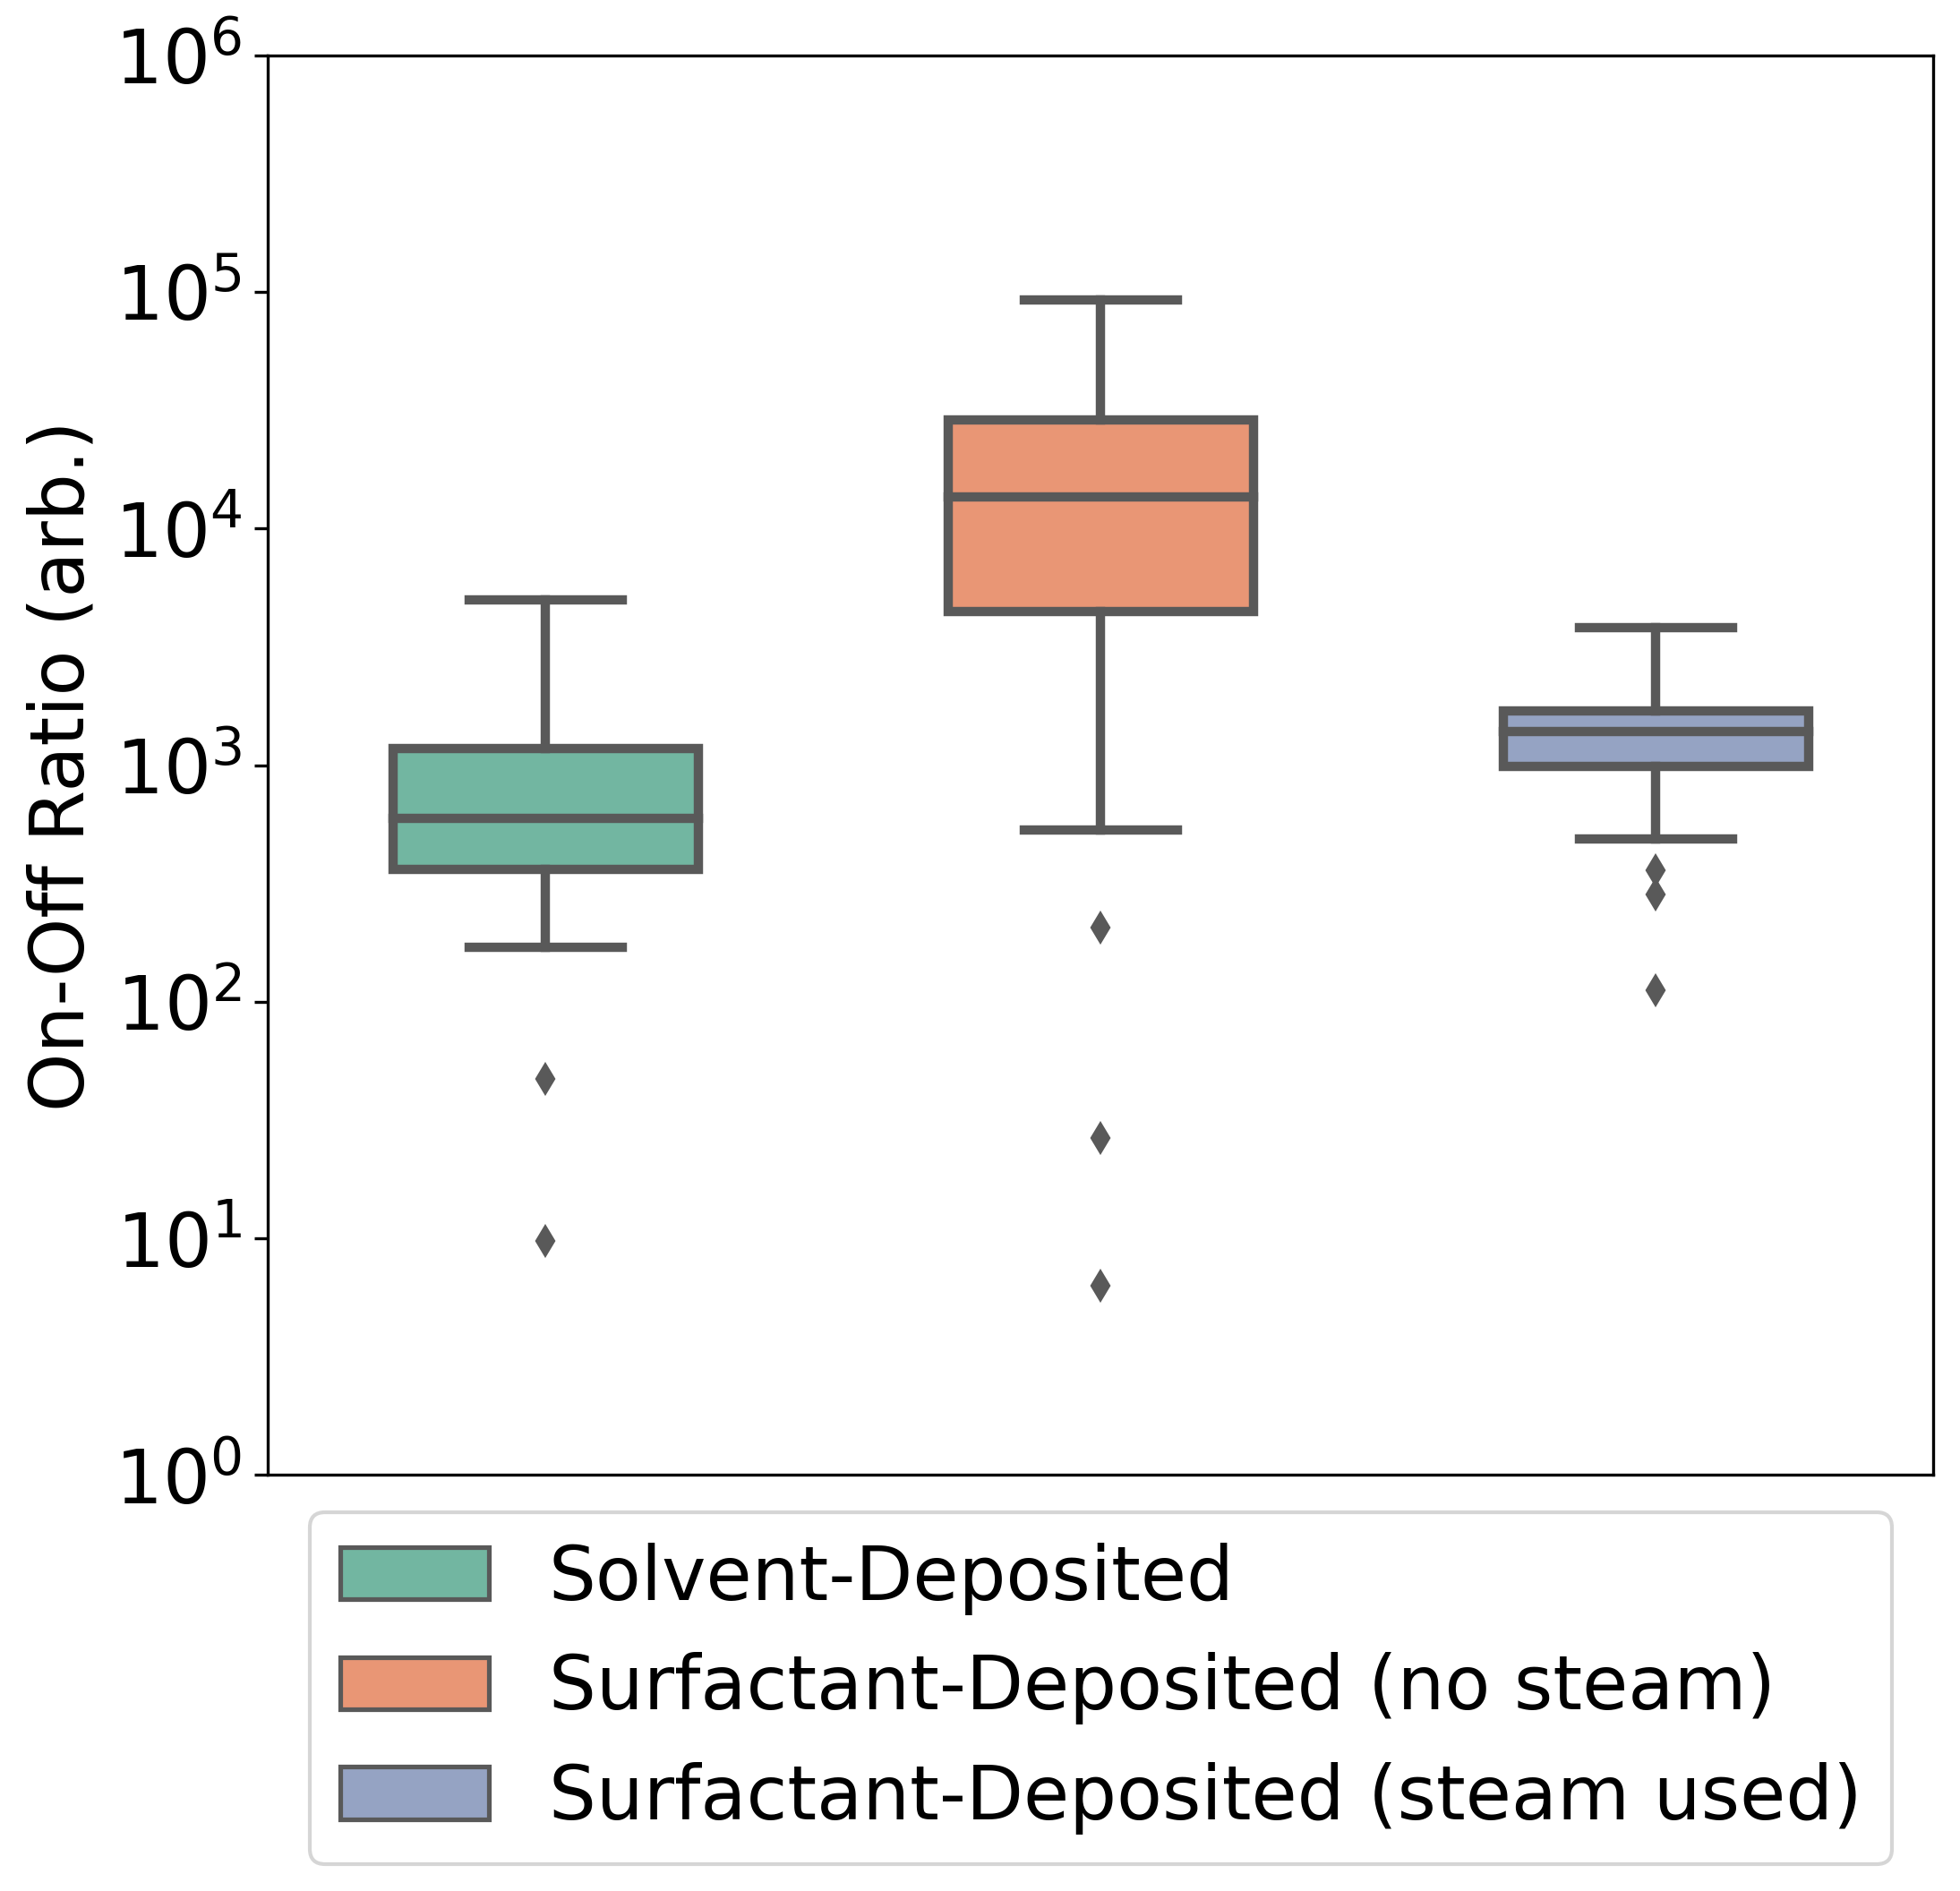
\includegraphics{./figures/ch5/onoff_CNT.png}

}

}

\subcaption{\label{fig-on-off-ratio}}
\end{minipage}%
%
\begin{minipage}[t]{0.05\linewidth}

{\centering 

~

}

\end{minipage}%
%
\begin{minipage}[t]{0.47\linewidth}

{\centering 

\raisebox{-\height}{

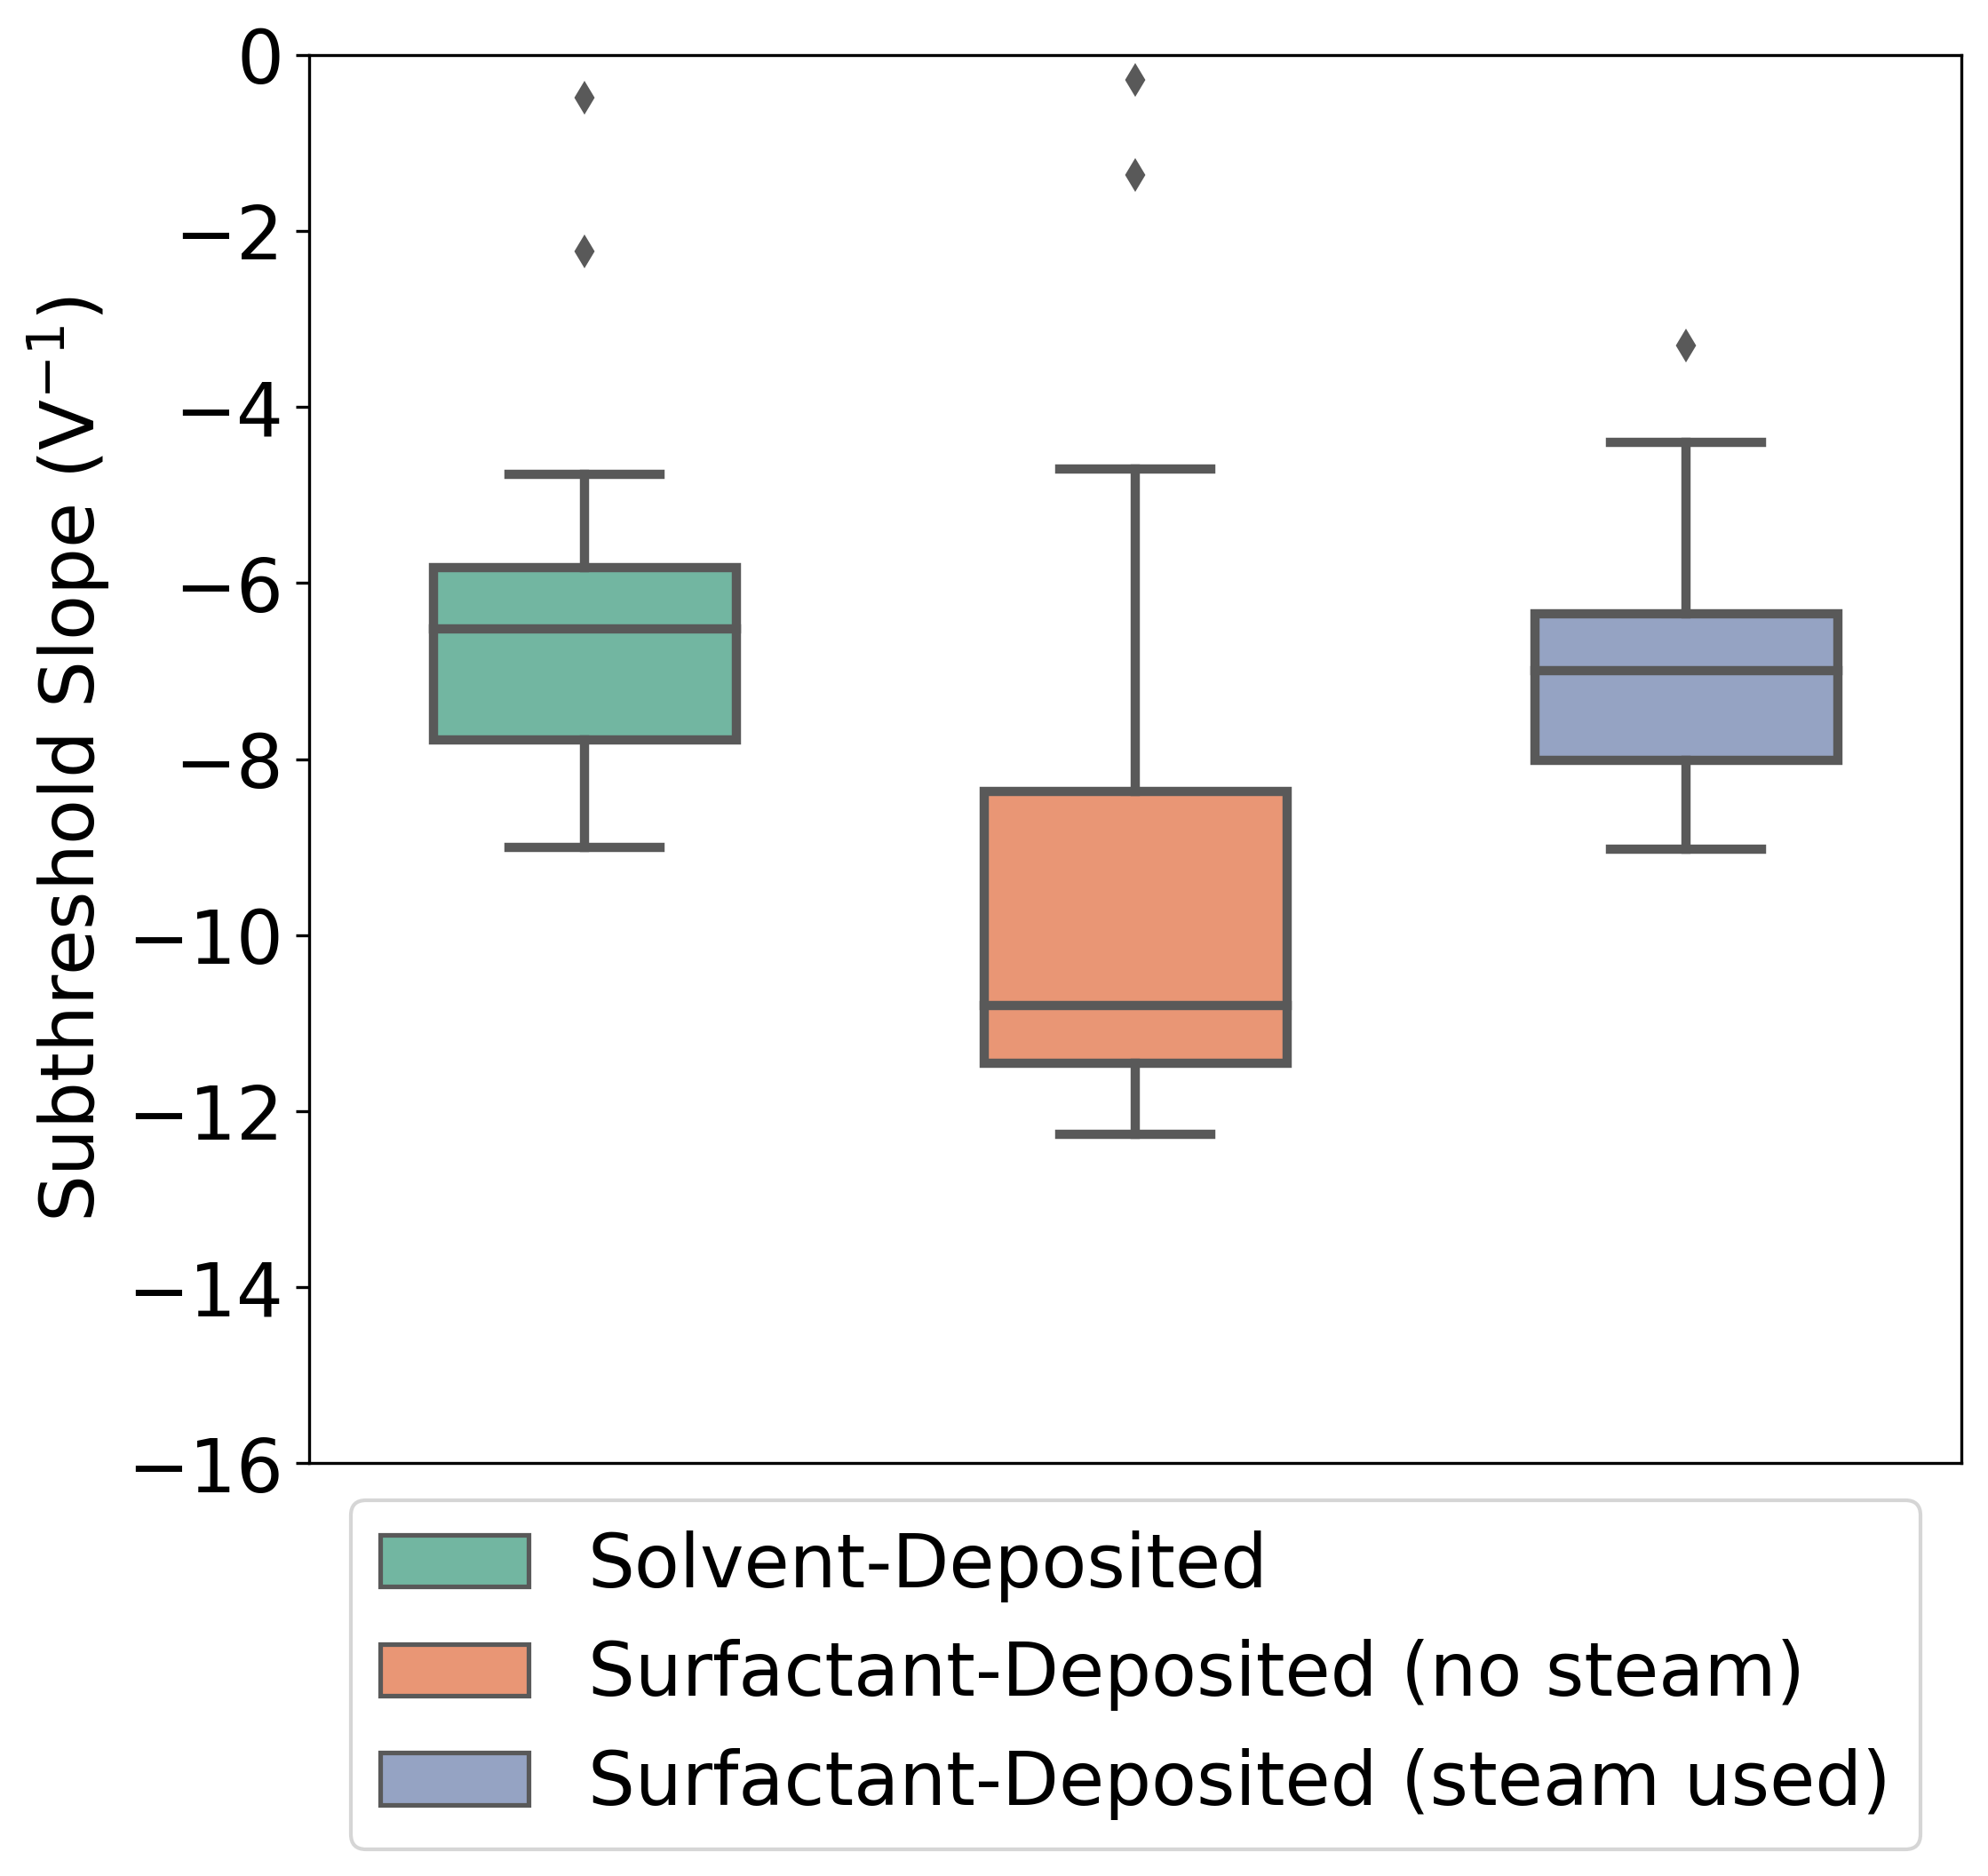
\includegraphics{./figures/ch5/SS.png}

}

}

\subcaption{\label{fig-subthreshold-slope}}
\end{minipage}%
\newline
\begin{minipage}[t]{0.26\linewidth}

{\centering 

~

}

\end{minipage}%
%
\begin{minipage}[t]{0.47\linewidth}

{\centering 

\raisebox{-\height}{

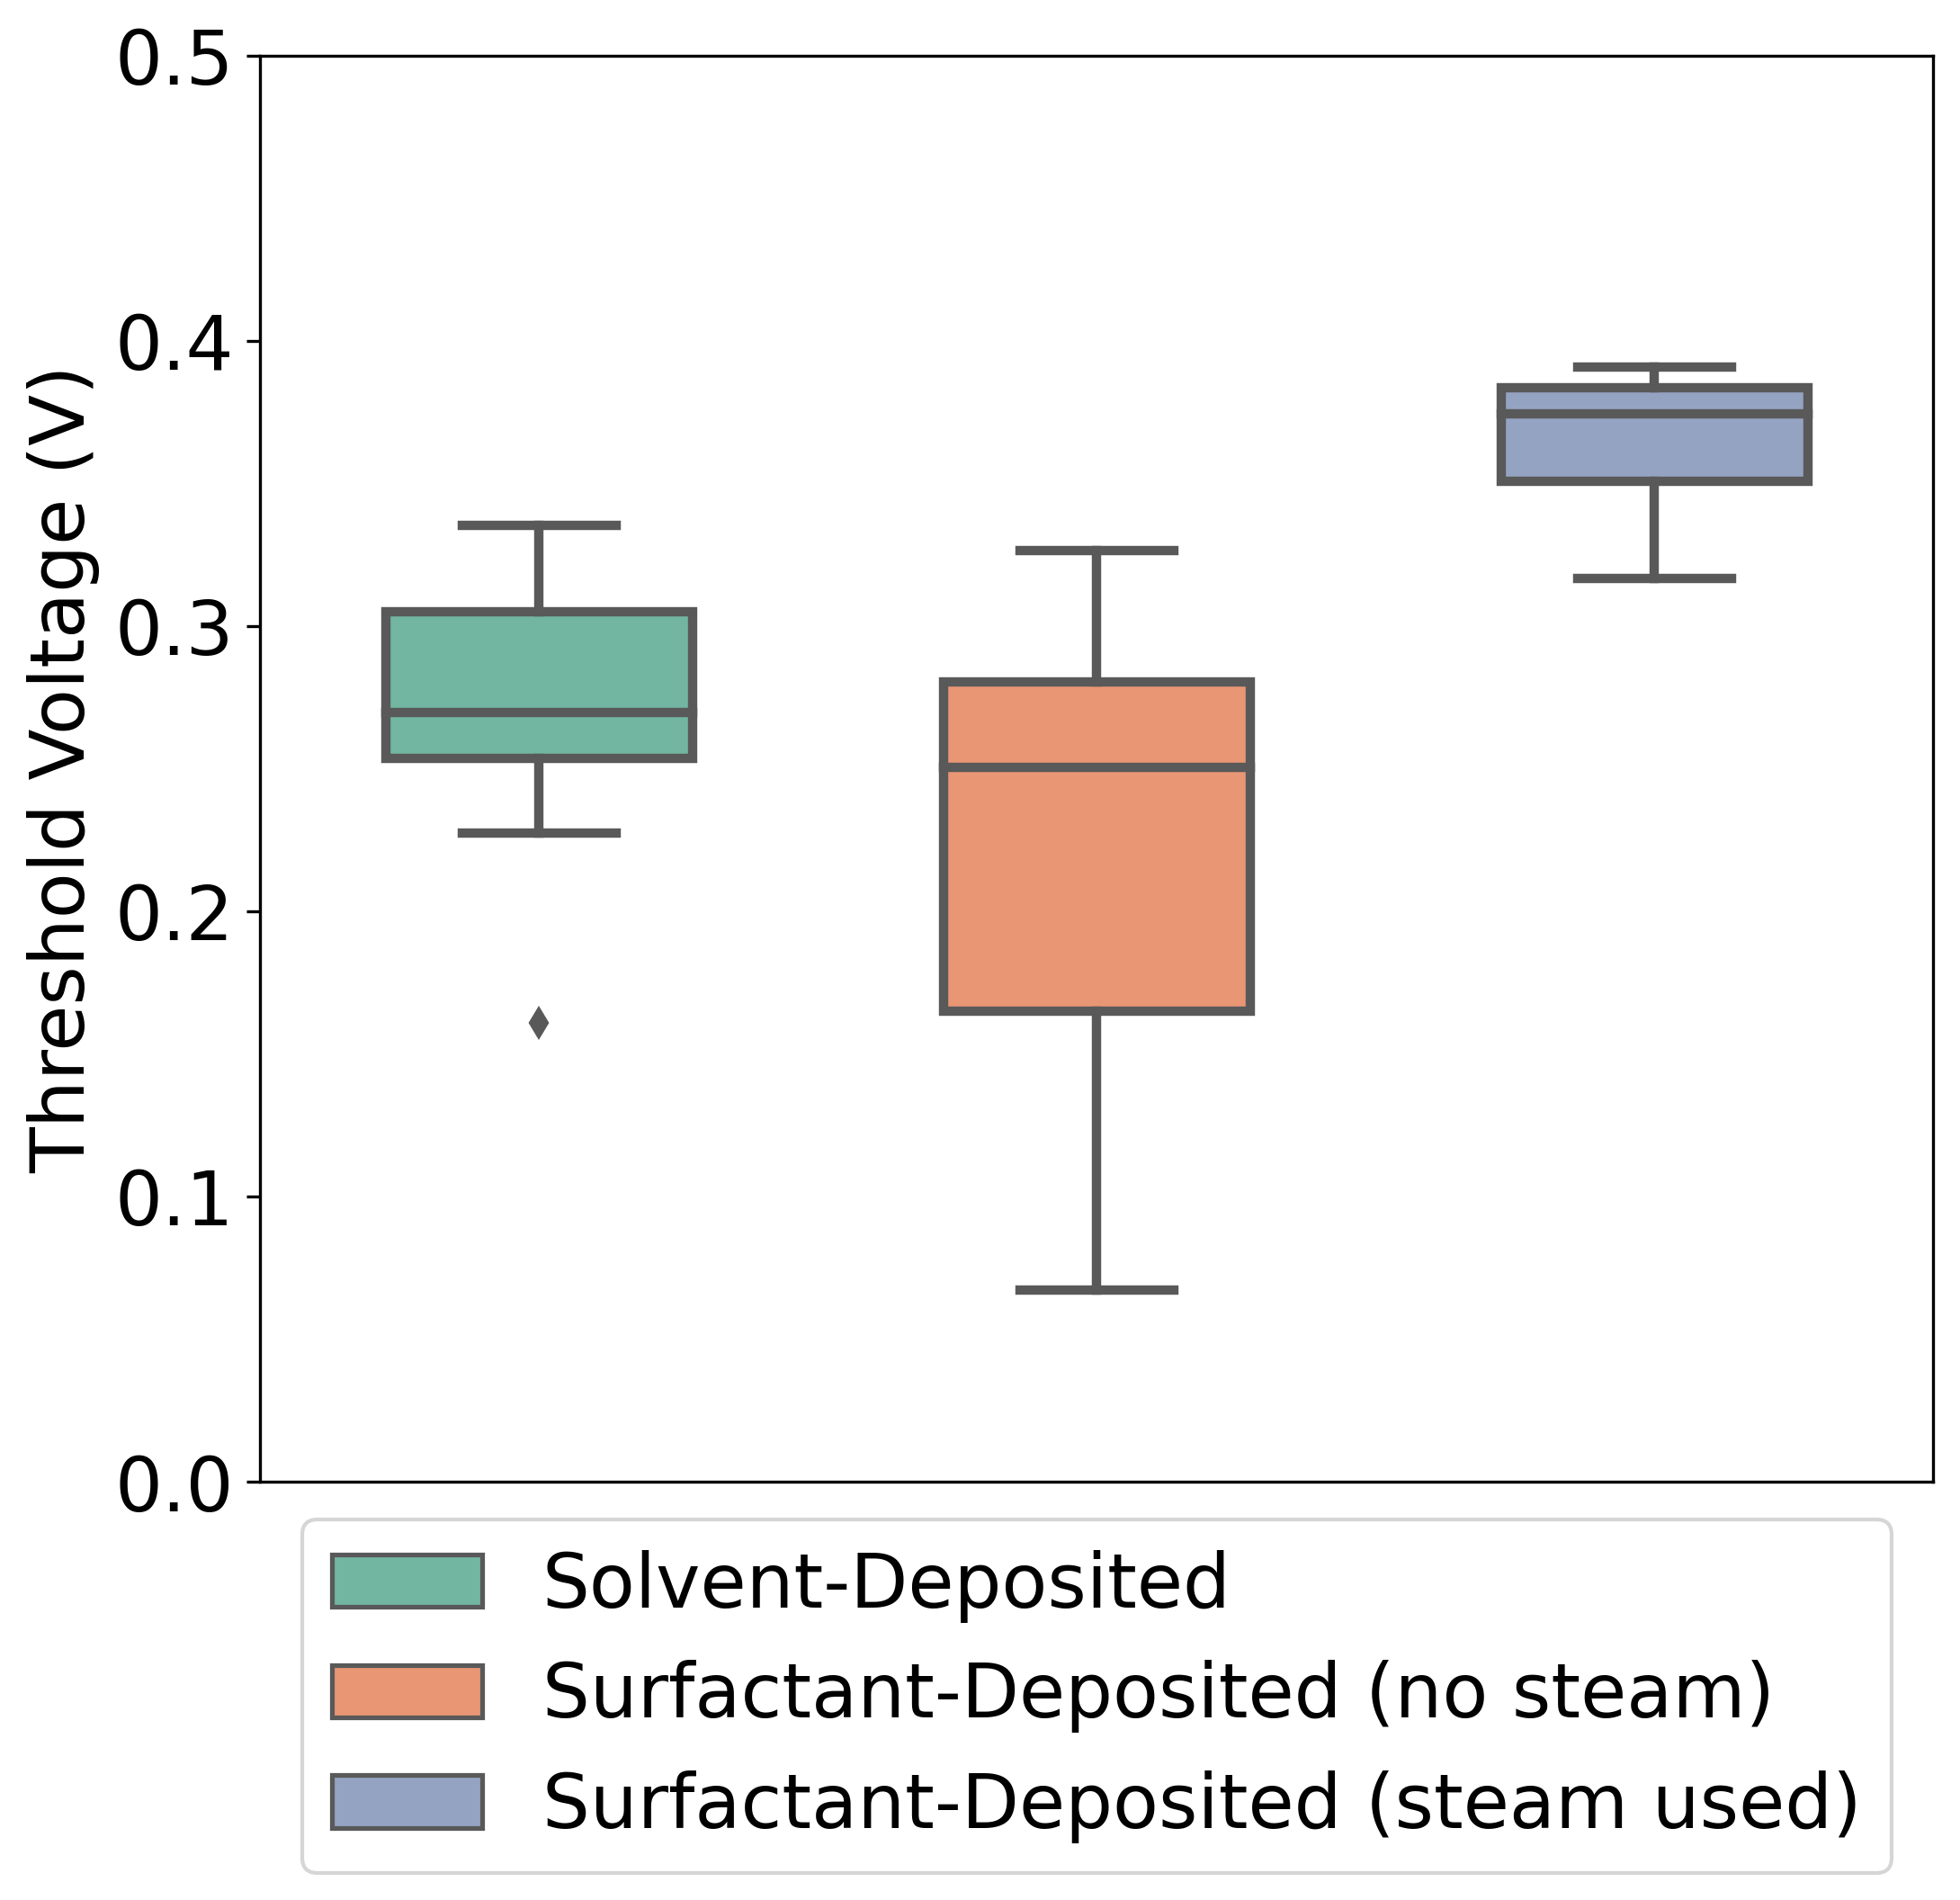
\includegraphics{./figures/ch5/threshold_V.png}

}

}

\subcaption{\label{fig-threshold-voltage}}
\end{minipage}%
%
\begin{minipage}[t]{0.26\linewidth}

{\centering 

~

}

\end{minipage}%

\caption{\label{fig-sweep-parameters}These boxplots illustrate the
statistical distribution of (a) the on-off ratio, (b) the subthreshold
slope, and (c) the threshold voltage of AZ\(^\circledR\) 1518
encapsulated liquid-gated transistor channels corresponding to each type
of carbon nanotube film deposition. For each deposition type, electrical
characteristics were taken of 21 channels of at least three separate
devices. The boxes indicate the 25th and 75th percentile of the
distribution.}

\end{figure}

When the devices were liquid-gated with 1XPBS electrolyte, they
exhibited ambipolar characteristics, commonly observed in carbon
nanotube network FETs
\autocite{Kauffman2008,Heller2009,JongYu2009,Derenskyi2014,Thanihaichelvan2018,Albarghouthi2022}.
Devices generally exhibited significantly less hysteresis than in the
backgated case. When devices were appropriately configured, leakage
current did not exceed \(\sim 1 \times 10^{-7}\) V across the forward
and reverse sweep. The devices shown which used carbon nanotube films
deposited in surfactant with steam present had significantly less
channel-to-channel variation in electrical characteristics than the
devices fabricated using other approaches. A summary of key parameters
of pristine liquid-gated devices is shown in
Figure~\ref{fig-sweep-parameters}. The full dataset consists of three
sets of 21 liquid-gated transfer characteristics of working channels,
with each set corresponding to the use of a particular method of carbon
nanotube network deposition in the device fabrication. Measurements from
at least three devices are included in each set. Each entry in the
summary corresponds to the average of the specific parameter in the
forward and reverse sweep direction.

Channels from surfactant-deposited film devices usually showed a larger
on-off ratio and subthreshold slope than those from solvent-deposited
devices. When the transistor is gated in the subthreshold range, a
larger on-off ratio and subthreshold slope results in a larger change in
conductance in response to changes in the transfer characteristic curve.
Therefore, a larger on-off ratio and subthreshold slope is desirable for
improved sensor performance \autocite{Kauffman2008,Heller2009,Gao2010}.
The larger on-off ratio for surfactant-deposited film devices is likely
a result of the reduced bundling of nanotubes, as discussed in
Section~\ref{sec-pristine-morphology}. Carbon nanotube pathways across
the channel with a lower degree of bundling will have a lower number of
component metallic tubes in the network, which increases the on-off
ratio \autocite{LeMieux2008,Rouhi2011,Thanihaichelvan2018}. The effect
of metallic nanotubes increasing the off current of a device channel is
illustrated by channel 1 in Figure~\ref{fig-solvent-tx-lg}. The larger
subthreshold slope is likely due to increased mobility from a denser
nanotube network in surfactant-deposited films \autocite{Rouhi2011}, as
seen in Figure~\ref{fig-afm-morphology}.

When steam is used for surfactant deposition of films, the resulting
devices showed highly consistent channel-to-channel electrical
properties. As the carbon nanotube films on these devices are relatively
dense, as seen in Figure~\ref{fig-afm-morphology}, we know that the
network is well above the percolation threshold. As many carbon nanotube
pathways connect across the channel in parallel, small variations in the
network morphology have less of an impact on the overall channel
behaviour \autocite{Thanihaichelvan2018}. We also see from
Table~\ref{tbl-histogram-parameters} that the range of bundle sizes is
relatively low in the steam-deposited films used in these devices. The
low range of bundle sizes means the semiconducting-metallic nanotube
ratio is far more consistent for these devices, leading to more
consistent electrical device characteristics. Being able to achieve
consistent subthreshold regime behaviour between channels on the same
device is a desirable attribute for reliable real-time multiplexed
biosensing \autocite{Kauffman2008,Heller2009,Gao2010}.

All channels characterised had a positive threshold voltage
(\(V_{th}\)). The threshold voltage was largest and most consistent for
steam-assisted surfactant-deposited films. The marked increase in
\(V_{th}\) for channel measurements from surfactant-deposited devices
with steam present relative to other channel measurements indicates
\(p\)-doping of the carbon nanotubes has occurred
\autocite{Heller2008,Thanihaichelvan2018}. It is highly likely the
dopant is present due to the steam deposition, and may be related to the
large contamination peak for steam-deposited films seen in
Figure~\ref{fig-afm-morphology} and
Figure~\ref{fig-remaining-histogram}. One possibility is that this
dopant is residual surfactant, which can \(p\)-dope carbon nanotubes and
lead to enhanced \(p\)-doping from adsorped oxygen and water
\autocite{Kane2014,Nonoguchi2018}. We have seen that steam prevents
bundling of carbon nanotubes during deposition. This effect is likely
due to persistence of the surfactant keeping nanotubes separate during
this process. Presence of surfactant may also explain the lowered
subthreshold slope and therefore mobility of the surfactant-deposited
devices with steam relative to the surfactant-deposited devices without
steam. The analysis by Kane \emph{et al.} shows that the thermal
annealling at 150\(^\circ\)C used in this work to remove residual
surfactant is likely inadequate for this purpose \autocite{Kane2014}.

\begin{figure}

\begin{minipage}[t]{0.47\linewidth}

{\centering 

\raisebox{-\height}{

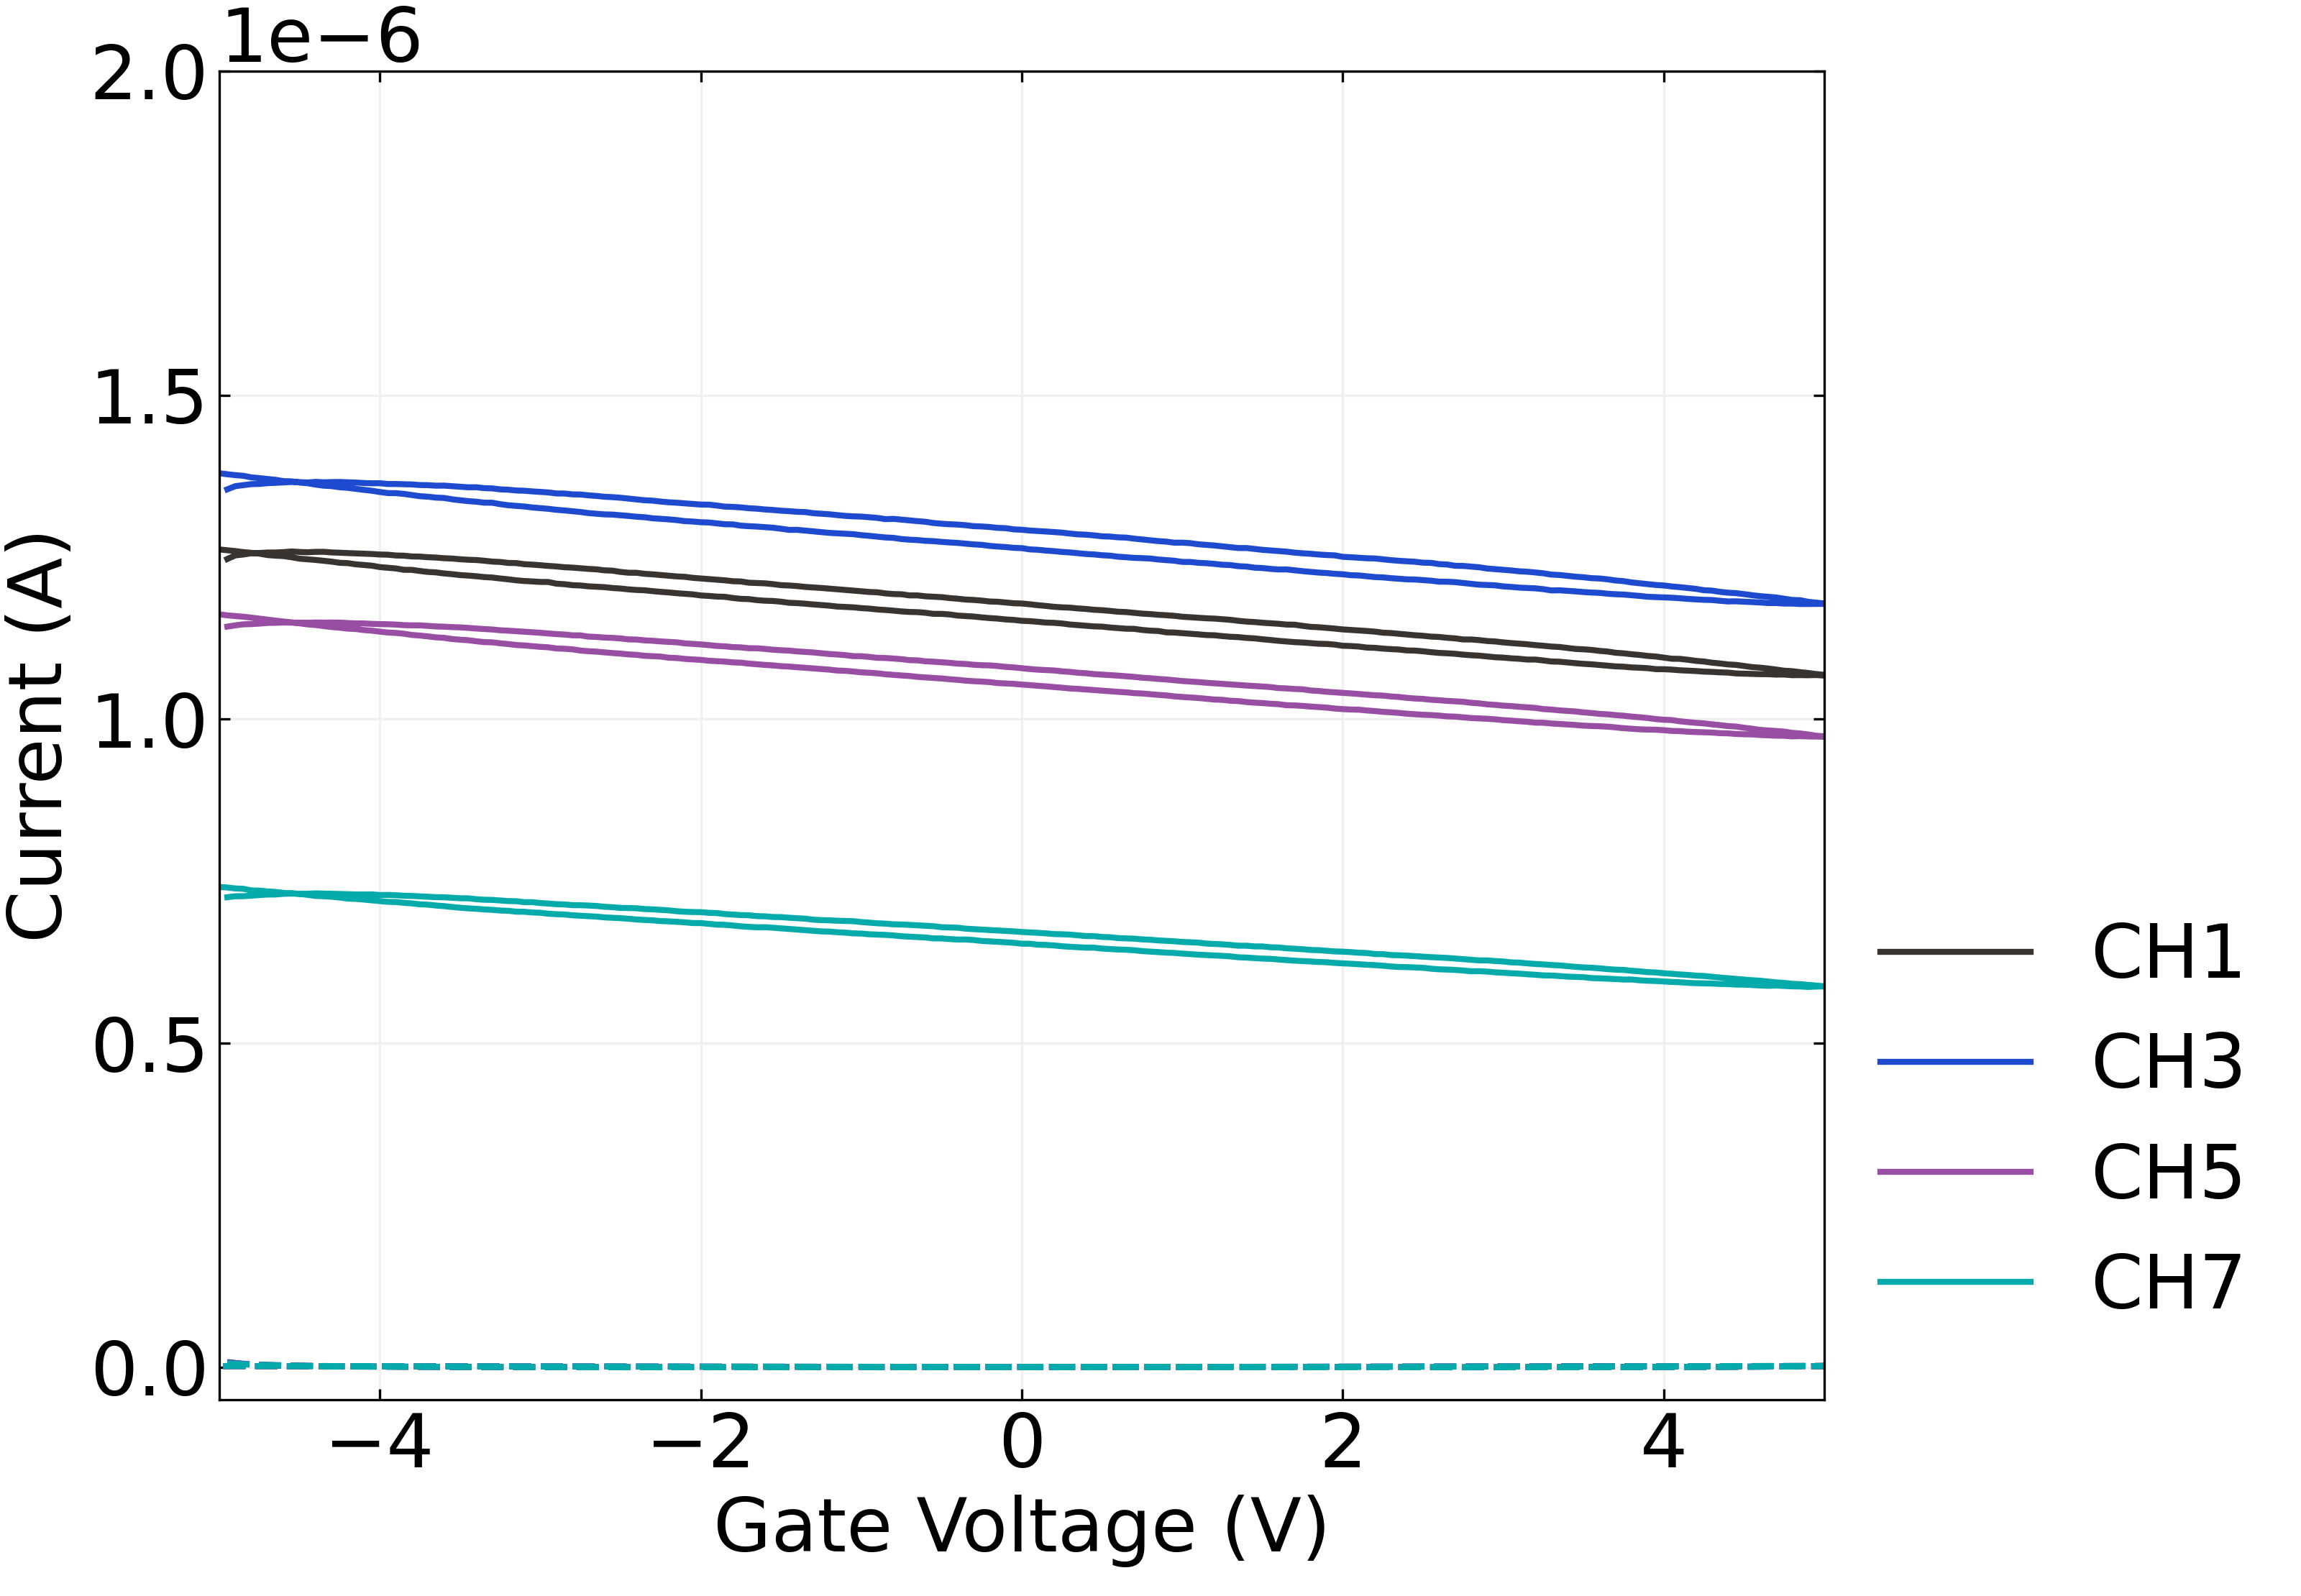
\includegraphics{./figures/ch5/Q35C3_nobuffer.png}

}

}

\subcaption{\label{fig-no-buffer}}
\end{minipage}%
%
\begin{minipage}[t]{0.05\linewidth}

{\centering 

~

}

\end{minipage}%
%
\begin{minipage}[t]{0.47\linewidth}

{\centering 

\raisebox{-\height}{

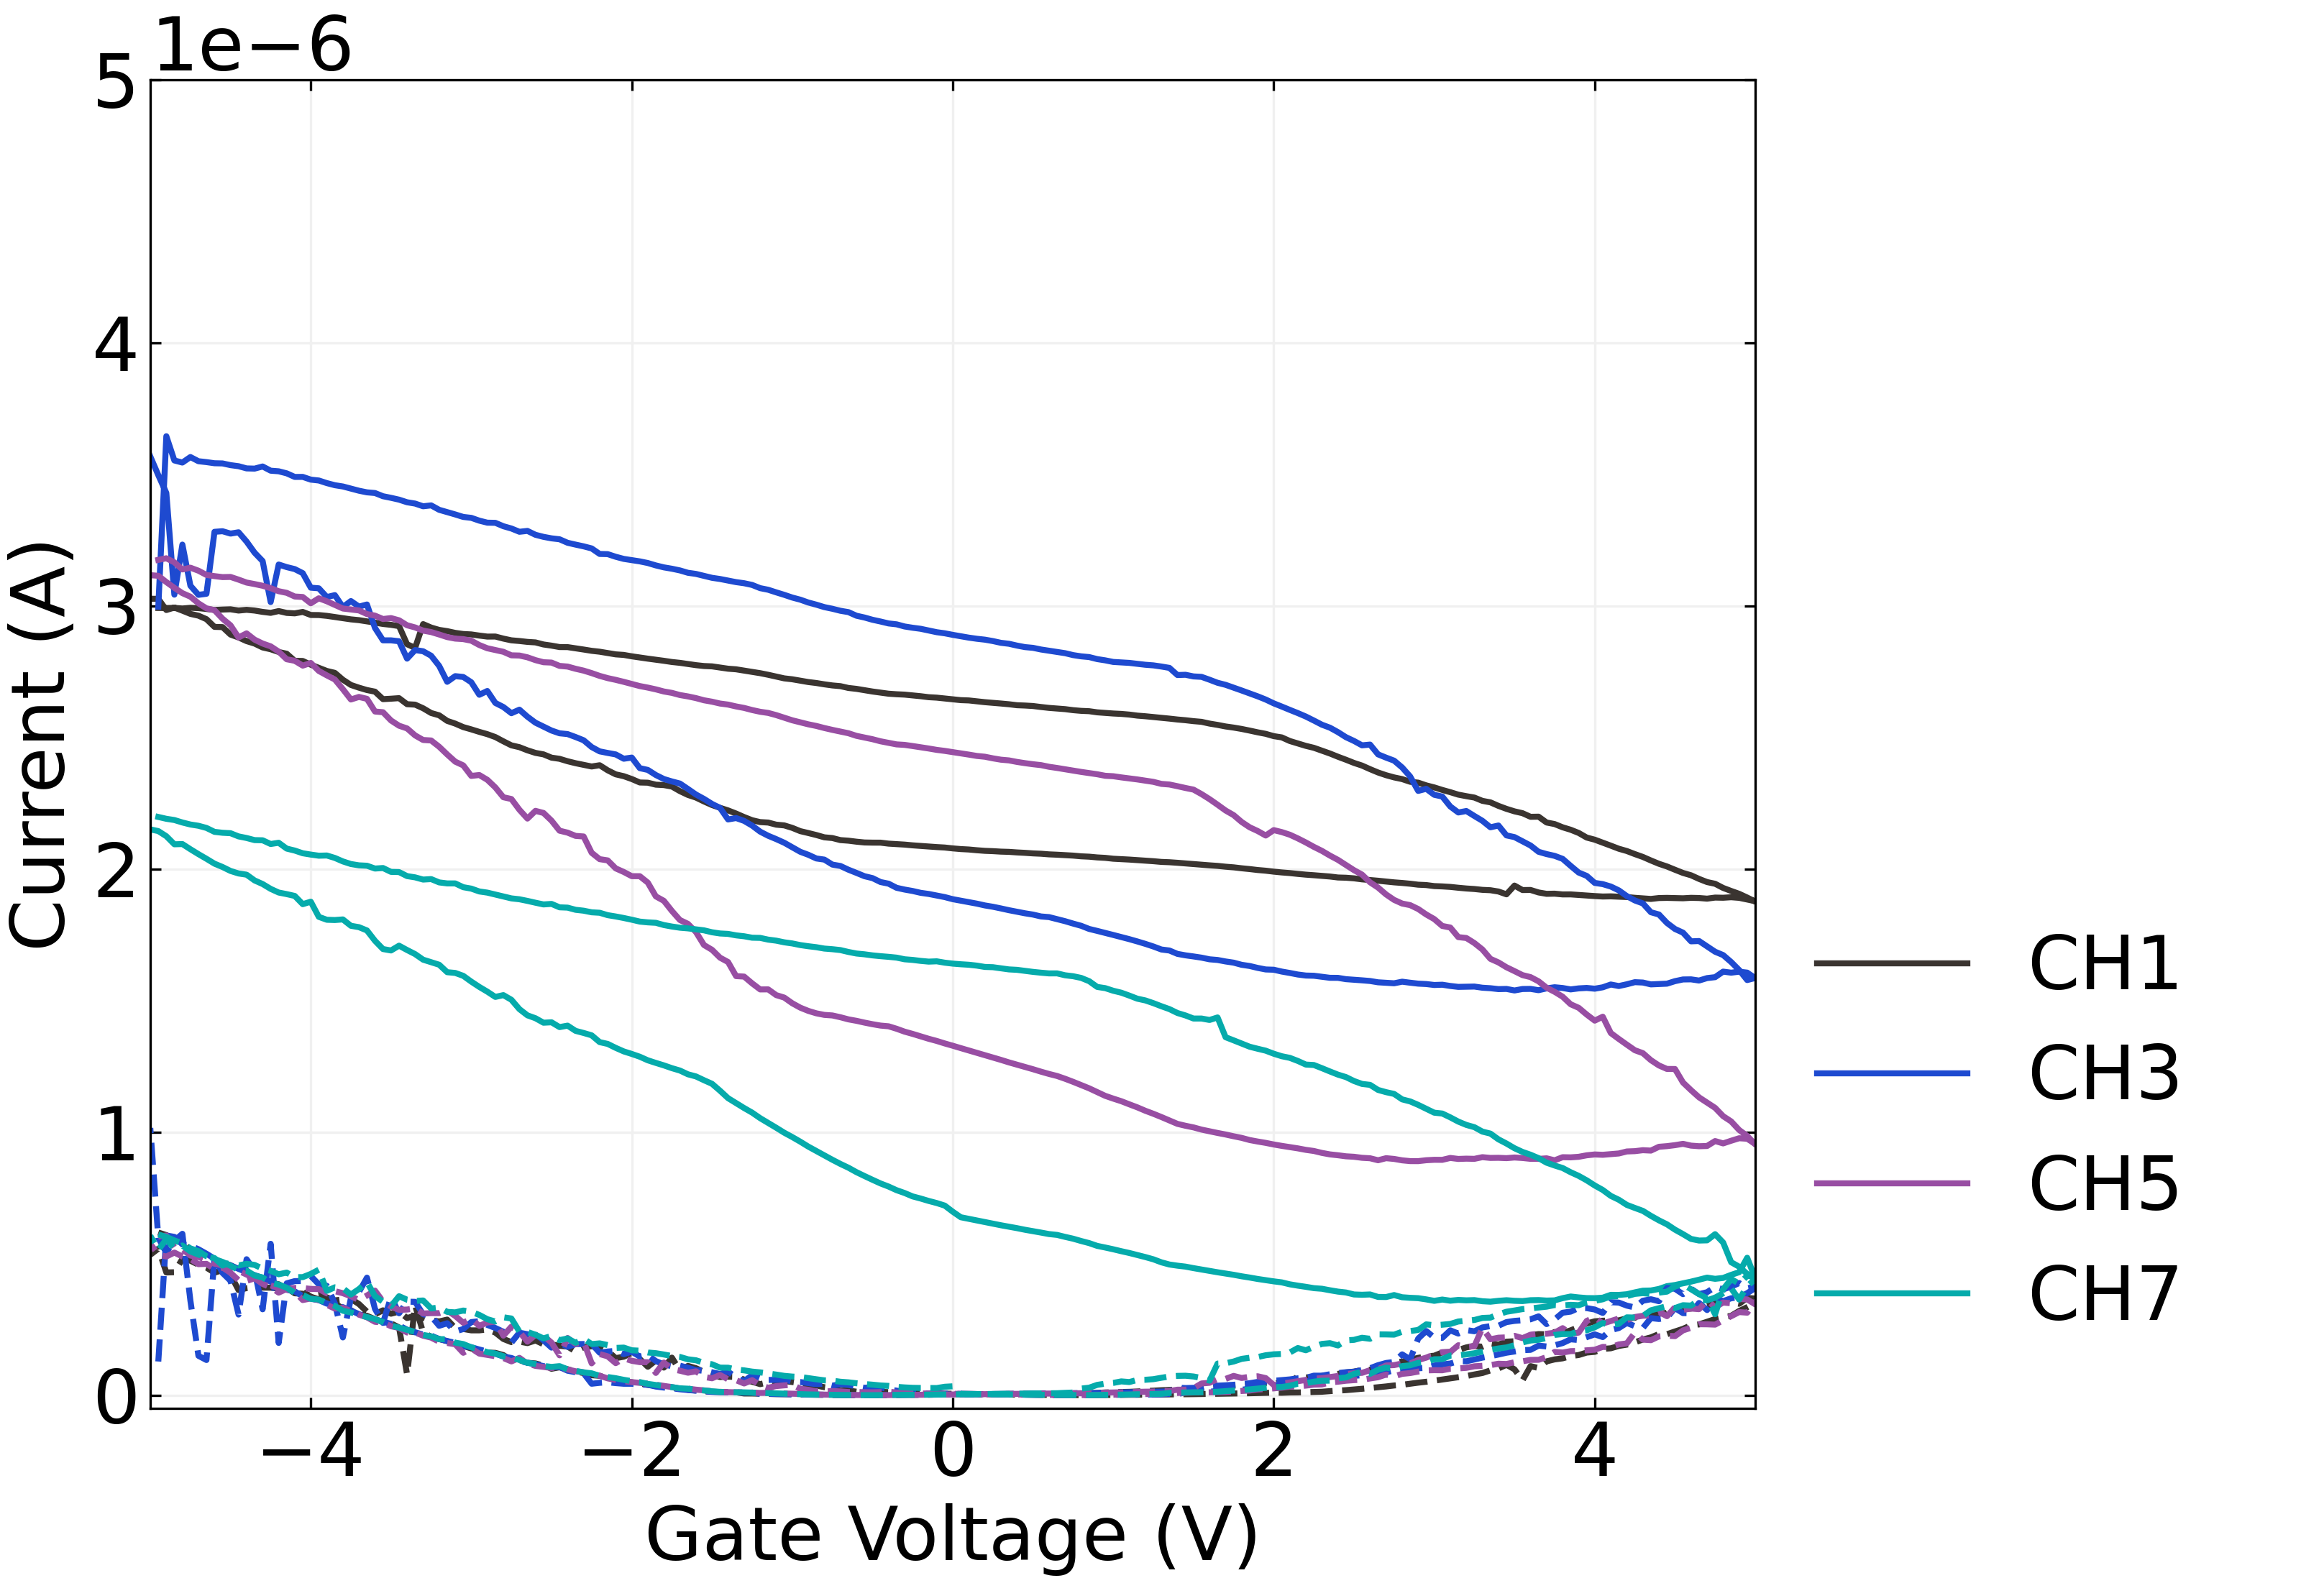
\includegraphics{./figures/ch5/Q35C3_buffer.png}

}

}

\subcaption{\label{fig-50uL-buffer}}
\end{minipage}%

\caption{\label{fig-buffer-effect-on-backgate}Backgated transfer sweeps
were taken of an single unencapsulated device with a 300 nm SiO\(_2\)
layer and steam assisted surfactant-deposited carbon nanotube network
channels before and after being covered in \(50 \mu\)L 1XPBS
electrolyte.}

\end{figure}

Figure~\ref{fig-buffer-effect-on-backgate} shows the behaviour of an
unencapsulated backgated device with a 300 nm SiO\(_2\) layer before and
after being covered by 50 \(\mu\)L of 1XPBS (phosphate buffered saline).
The on-off ratio and hysteresis of the channels increase significantly.
The presence of water increases hysteresis through introducing charge
traps at the silicon dioxide surface around the carbon nanotubes and at
the surface of the nanotubes themselves
\autocite{Kim2003,Lee2007,Ha2014}. The use of alternative transistor
dielectrics and/or device functionalisation could potentially be used to
reduce this hysteresis, as the time variation in threshold voltage due
to hysteresis is unwanted for biosensing work \autocite{Lee2007,Ha2014}.
The electrical double layer formed by the electrolyte at the surface of
the carbon nanotubes will also have contributed to the observed change
in electrical properties, as it screens surface charge present on the
surface around the nanotubes \autocite{Heller2010}.

There is also a significant increase in current leakage to the backgate
for larger applied voltages, despite the electrolyte having no visible
physical contact with the silicon backgate or copper plane. This leakage
current may simply be due to an increase in relative humidity around the
device due to the presence of water \autocite{Conseil2014}.

\hypertarget{graphene}{%
\subsection{Graphene}\label{graphene}}

\begin{figure}

\begin{minipage}[t]{0.47\linewidth}

{\centering 

\raisebox{-\height}{

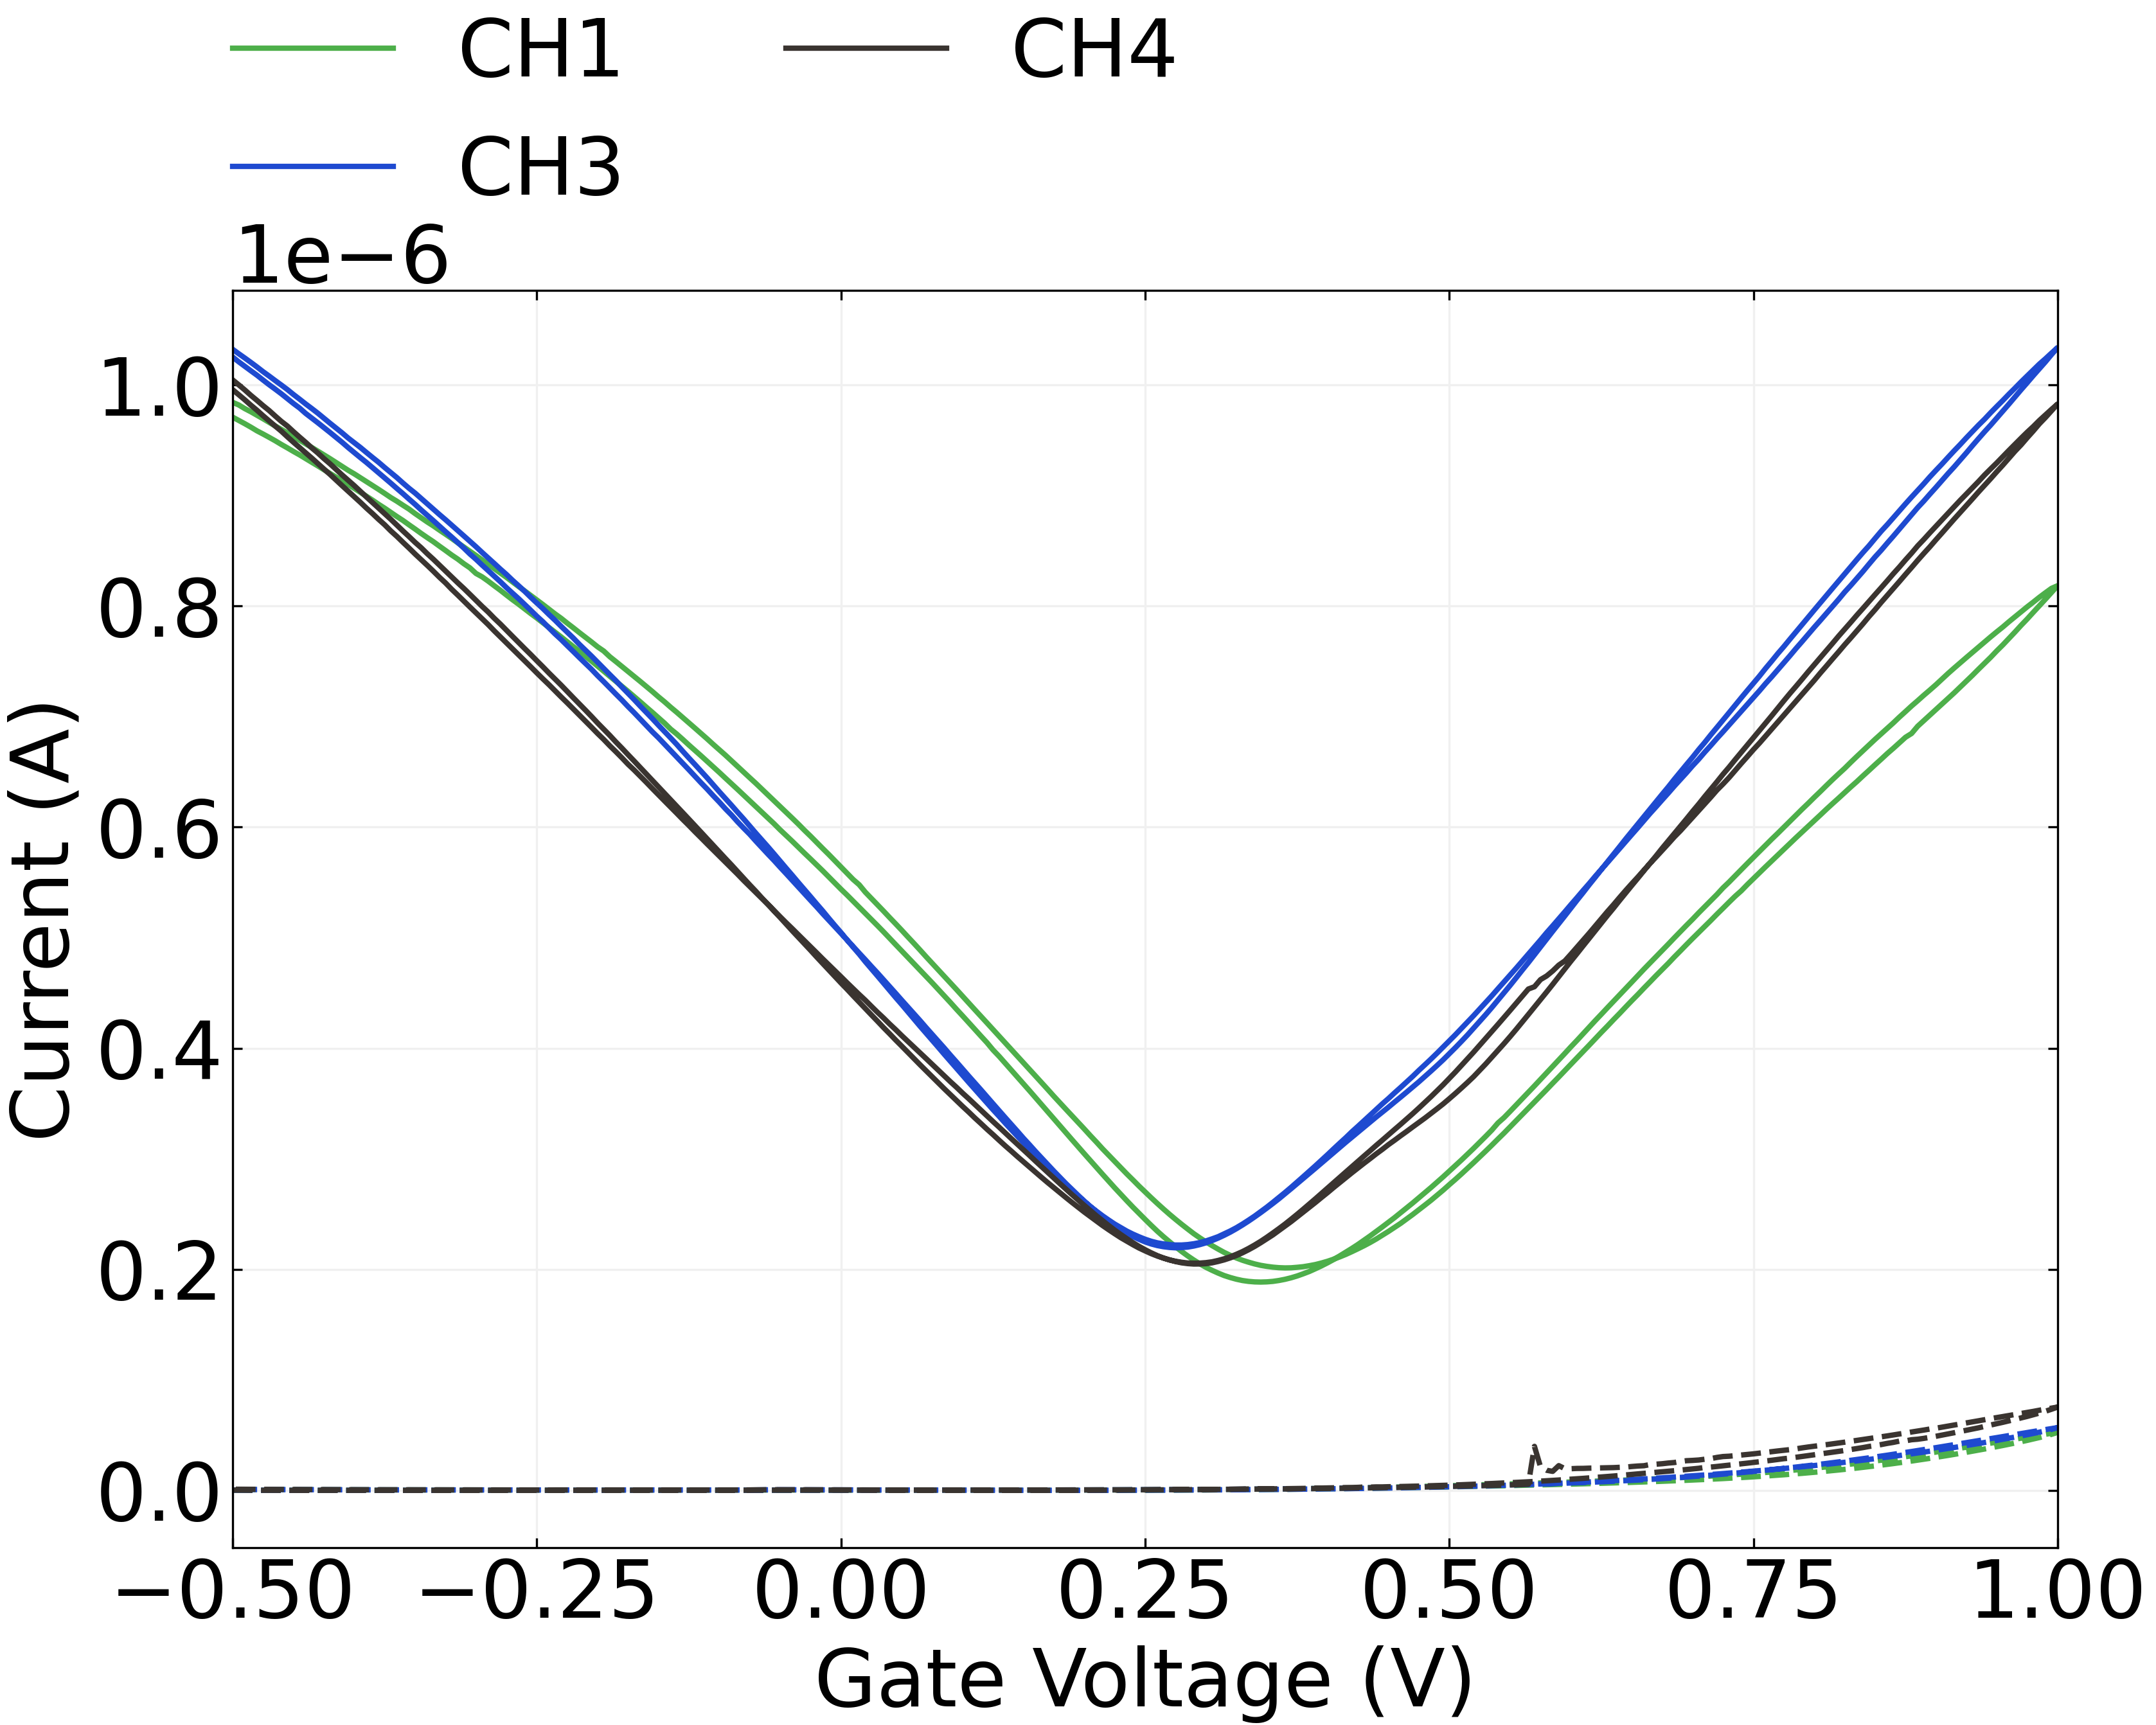
\includegraphics{./figures/ch5/JG098_pristine_TXLG01_5mVstep_220920_norinse.png}

}

}

\subcaption{\label{fig-graphene-transfer-1}}
\end{minipage}%
%
\begin{minipage}[t]{0.05\linewidth}

{\centering 

~

}

\end{minipage}%
%
\begin{minipage}[t]{0.47\linewidth}

{\centering 

\raisebox{-\height}{

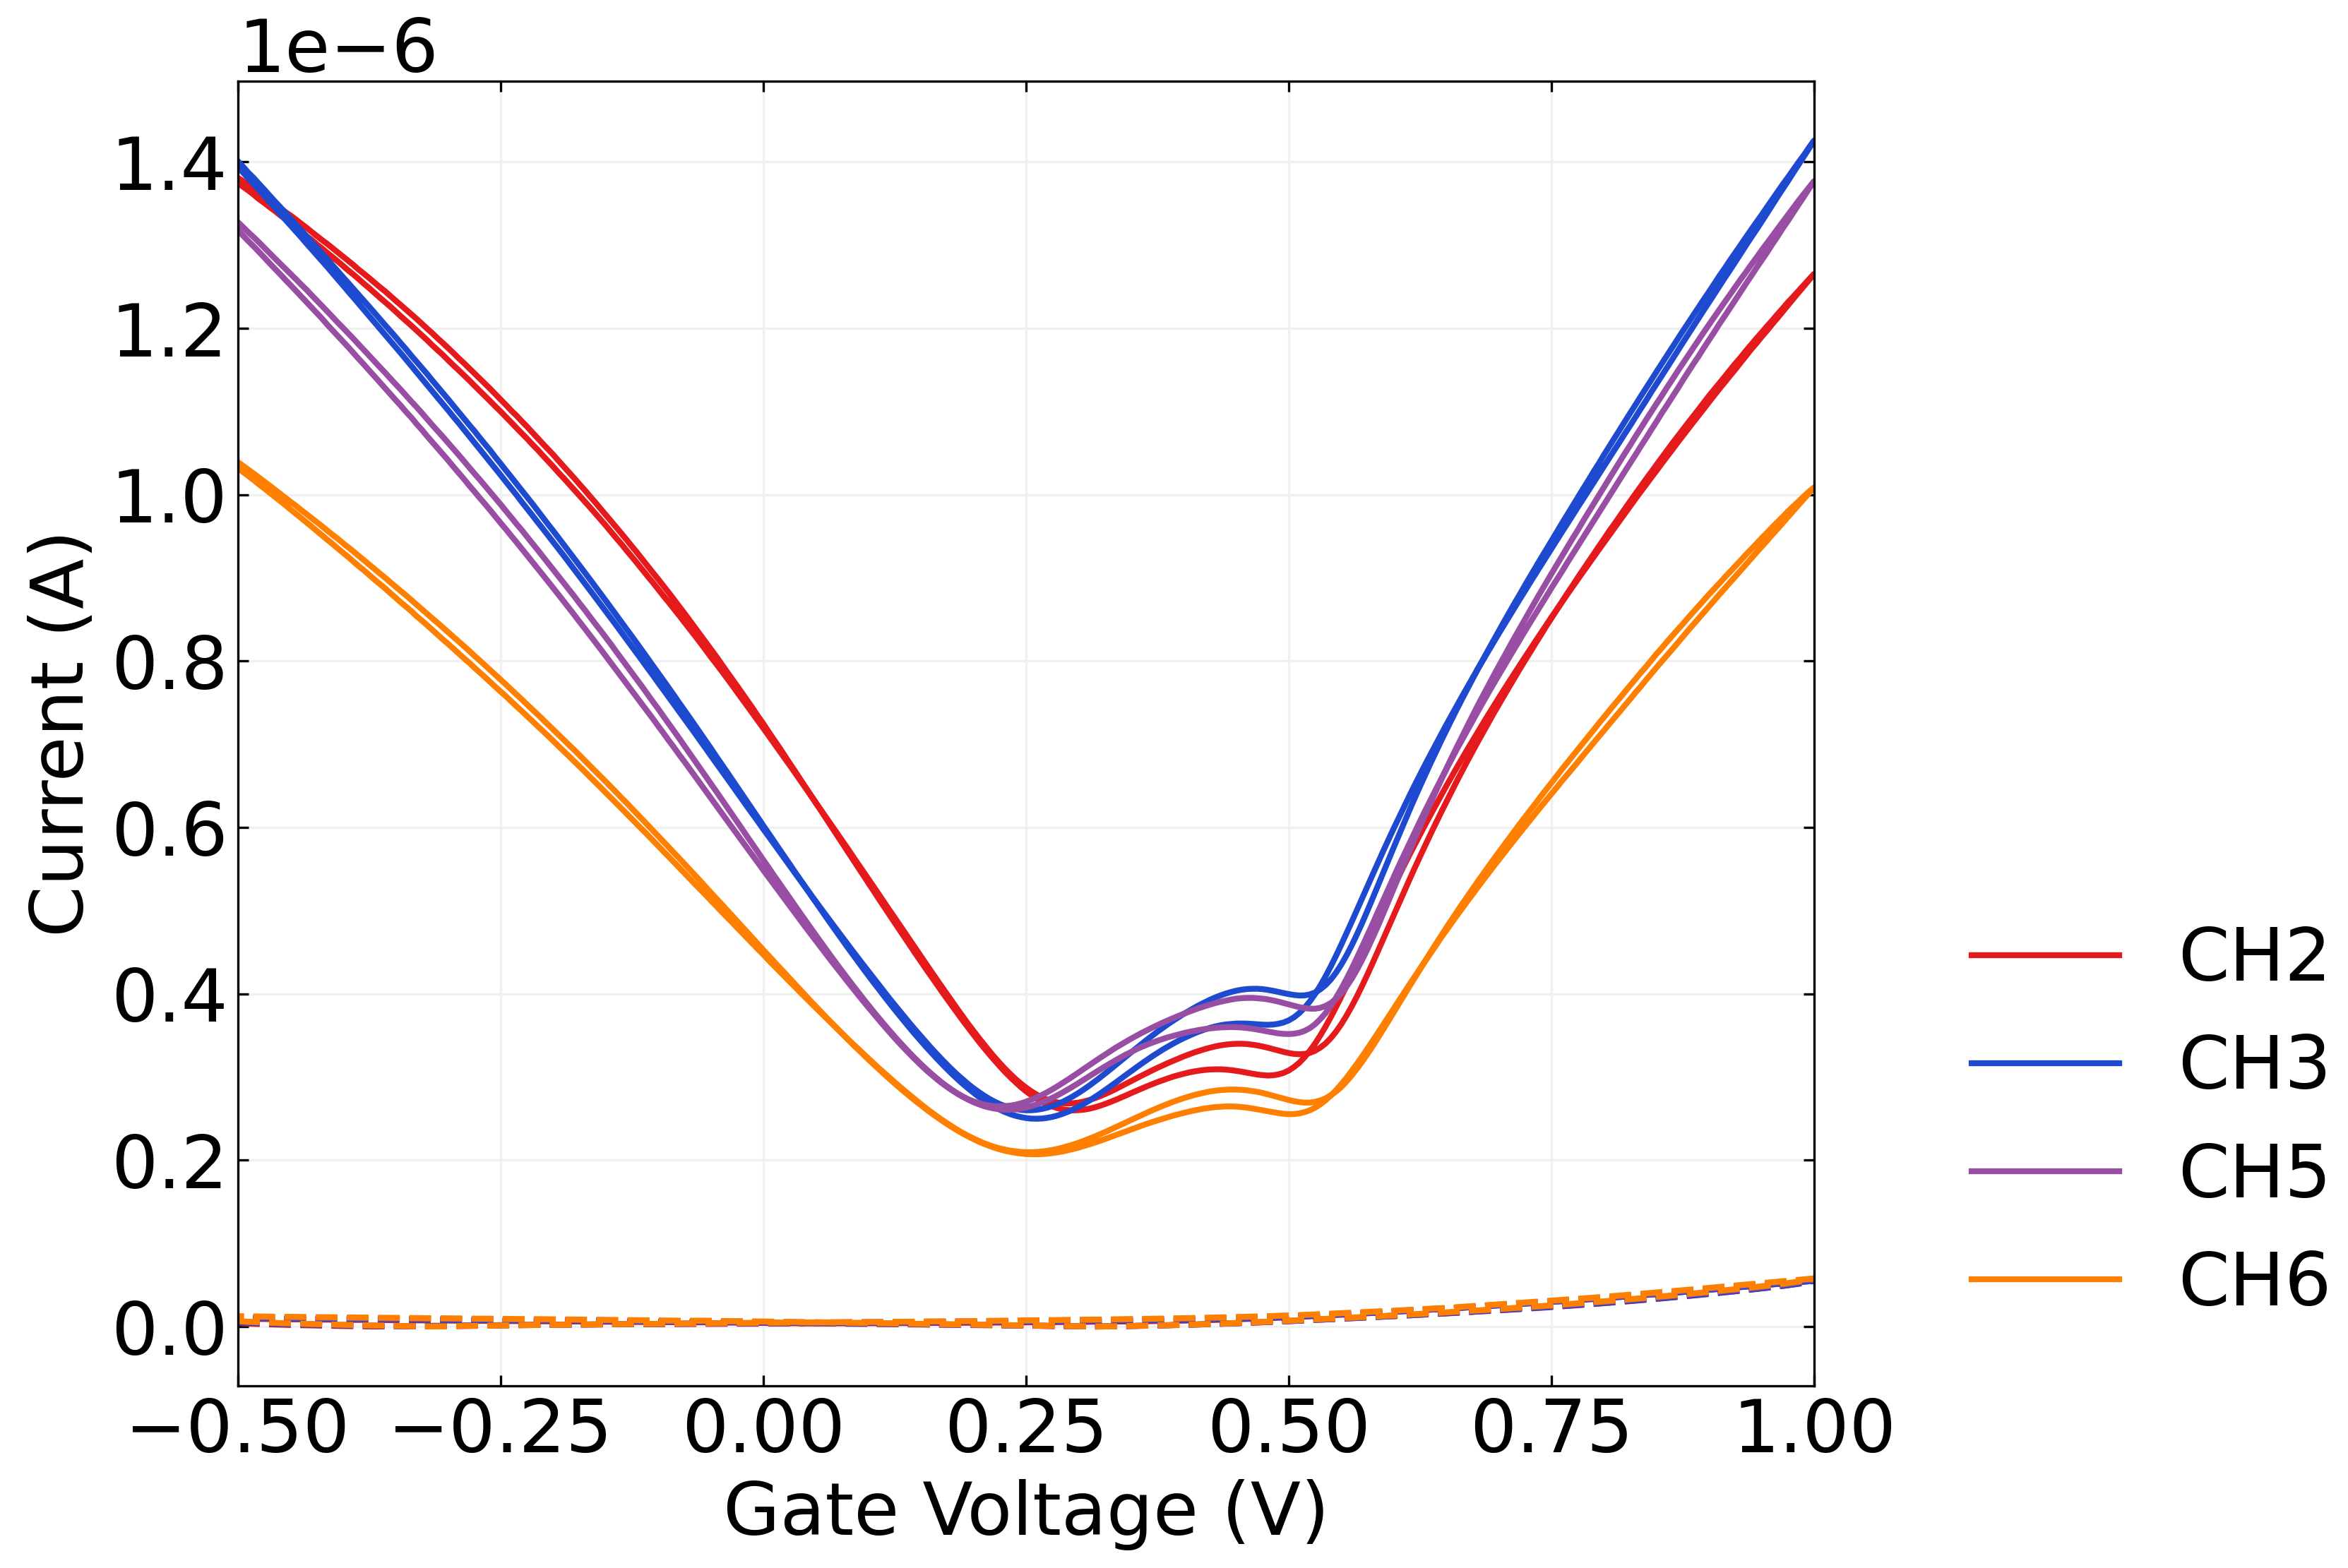
\includegraphics{./figures/ch5/JGQ00D6_pristine_TXLG01_5mVstep_220914_norinse.png}

}

}

\subcaption{\label{fig-graphene-transfer-2}}
\end{minipage}%
\newline
\begin{minipage}[t]{0.47\linewidth}

{\centering 

\raisebox{-\height}{

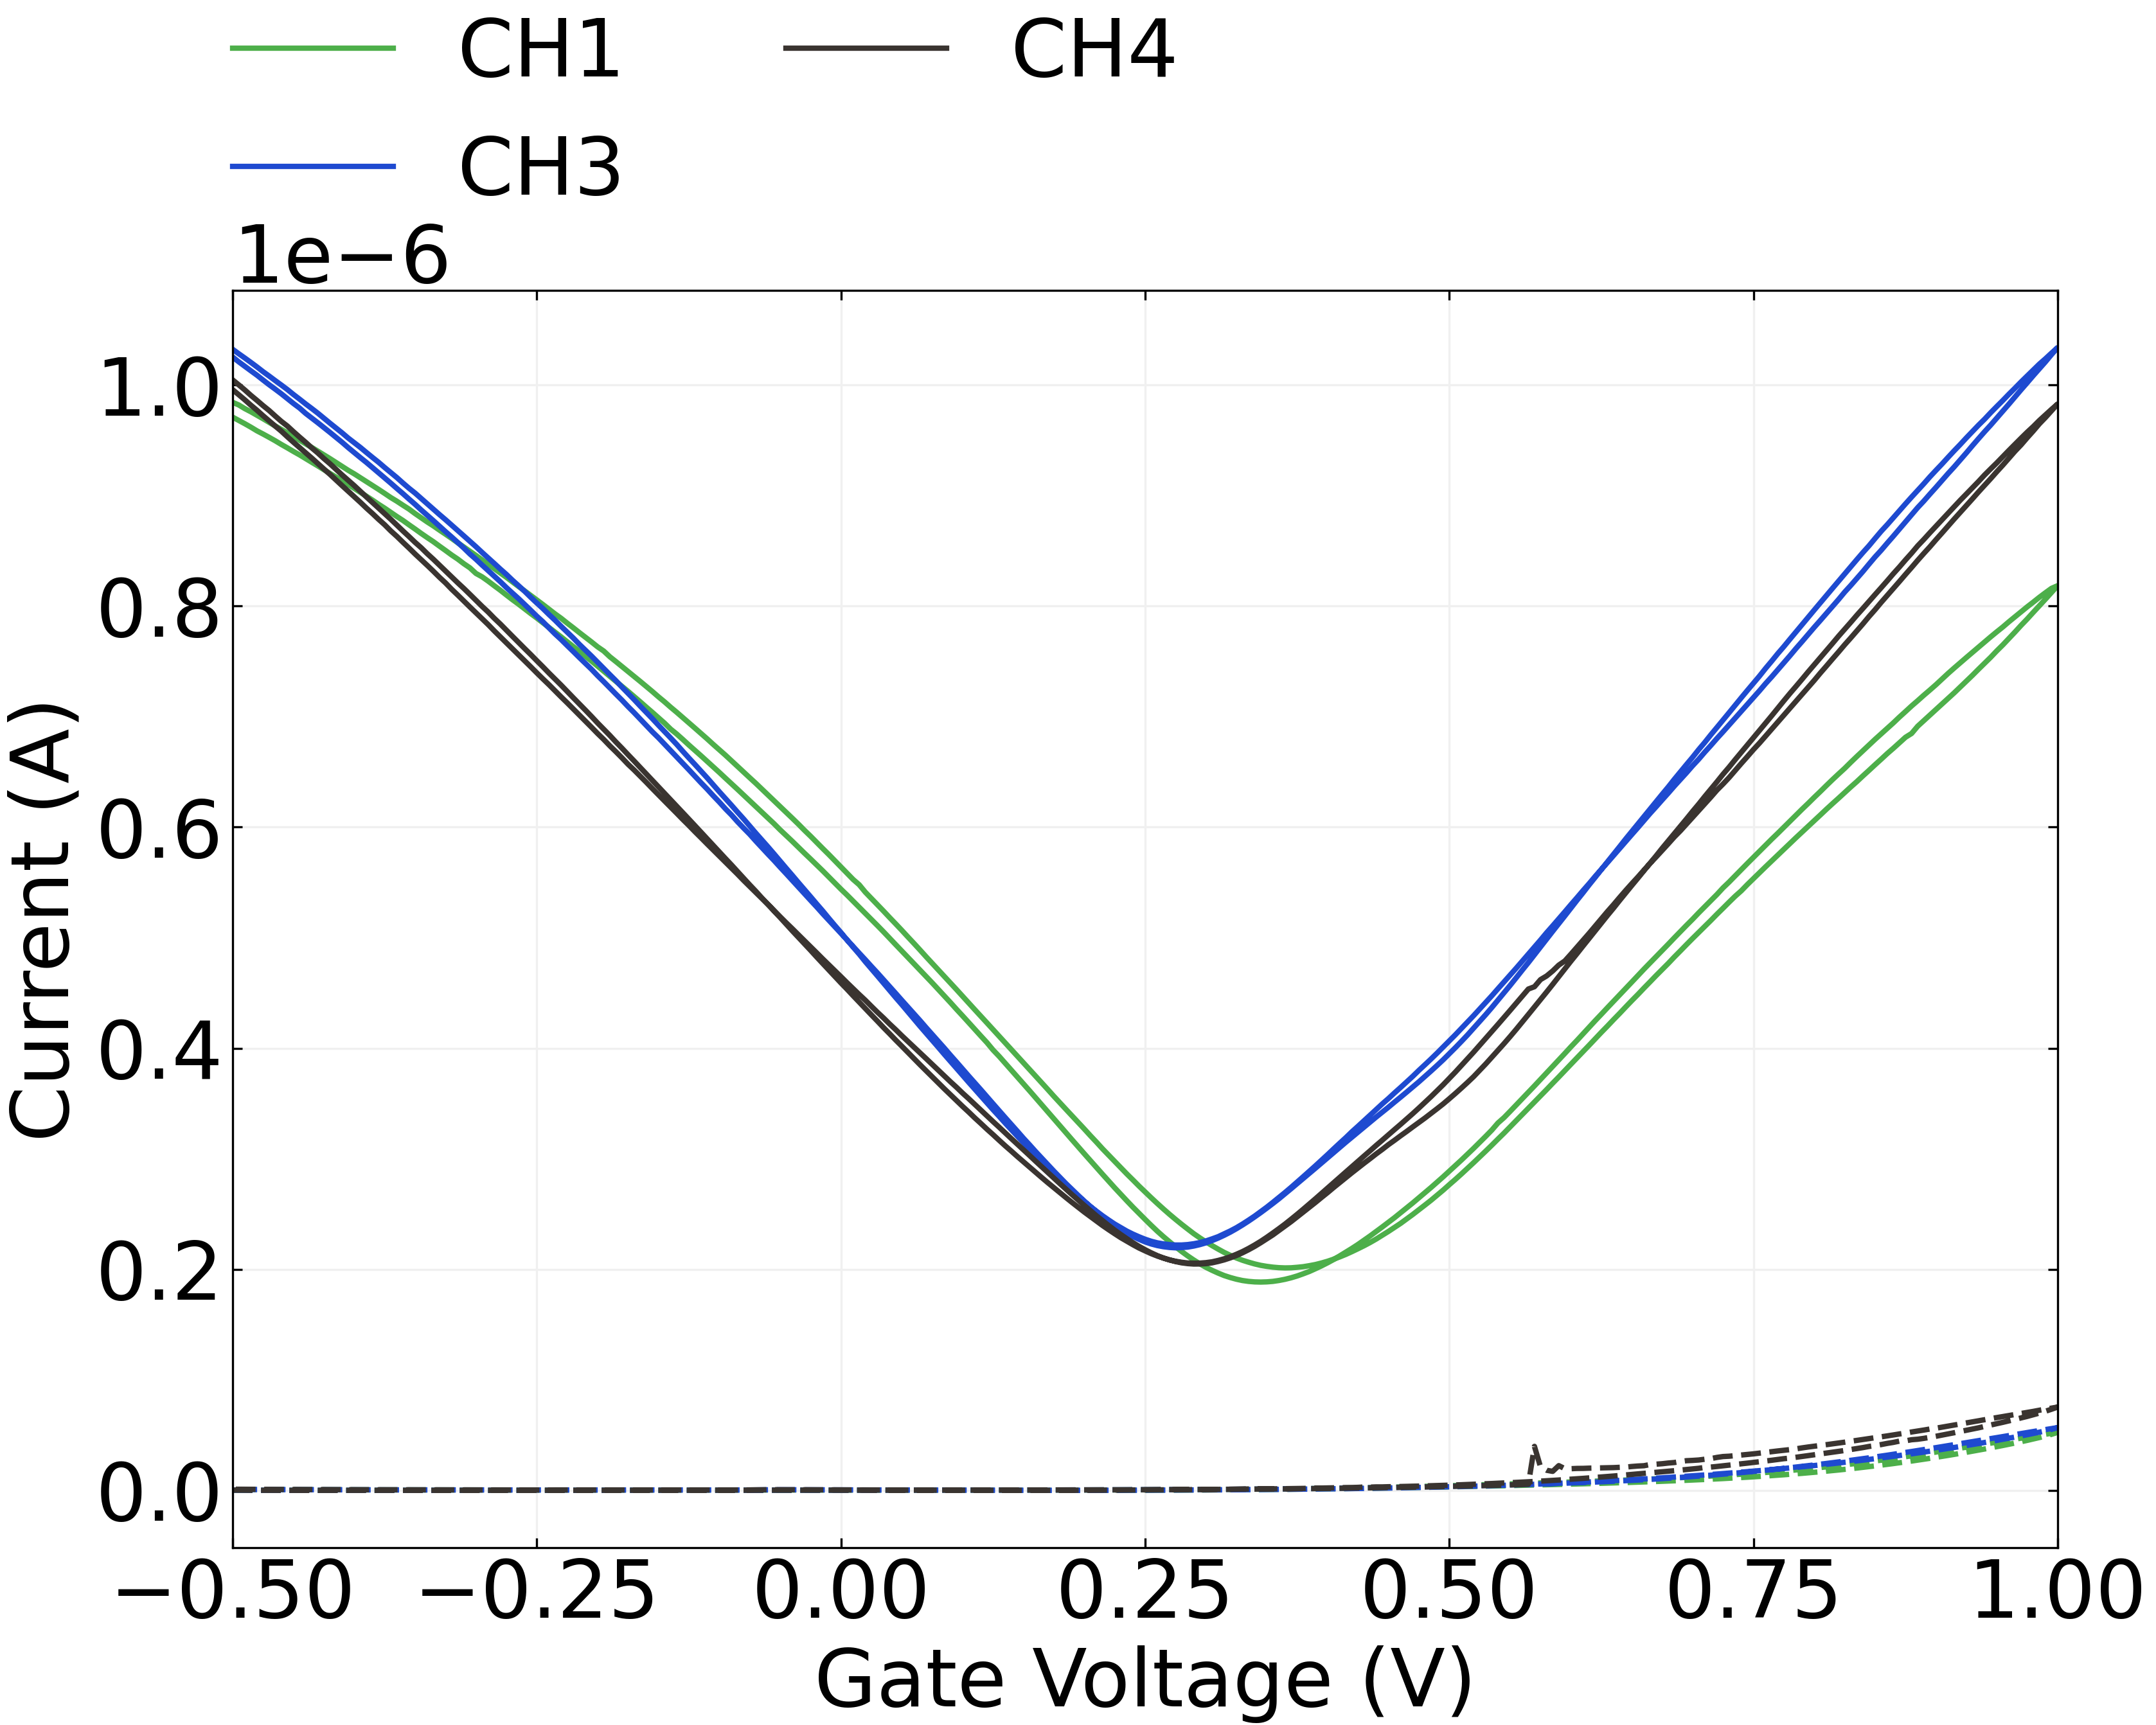
\includegraphics{./figures/ch5/JG098_pristine_TXLG01_5mVstep_220920_norinse.png}

}

}

\subcaption{\label{fig-x-voltage}}
\end{minipage}%
%
\begin{minipage}[t]{0.05\linewidth}

{\centering 

~

}

\end{minipage}%
%
\begin{minipage}[t]{0.47\linewidth}

{\centering 

\raisebox{-\height}{

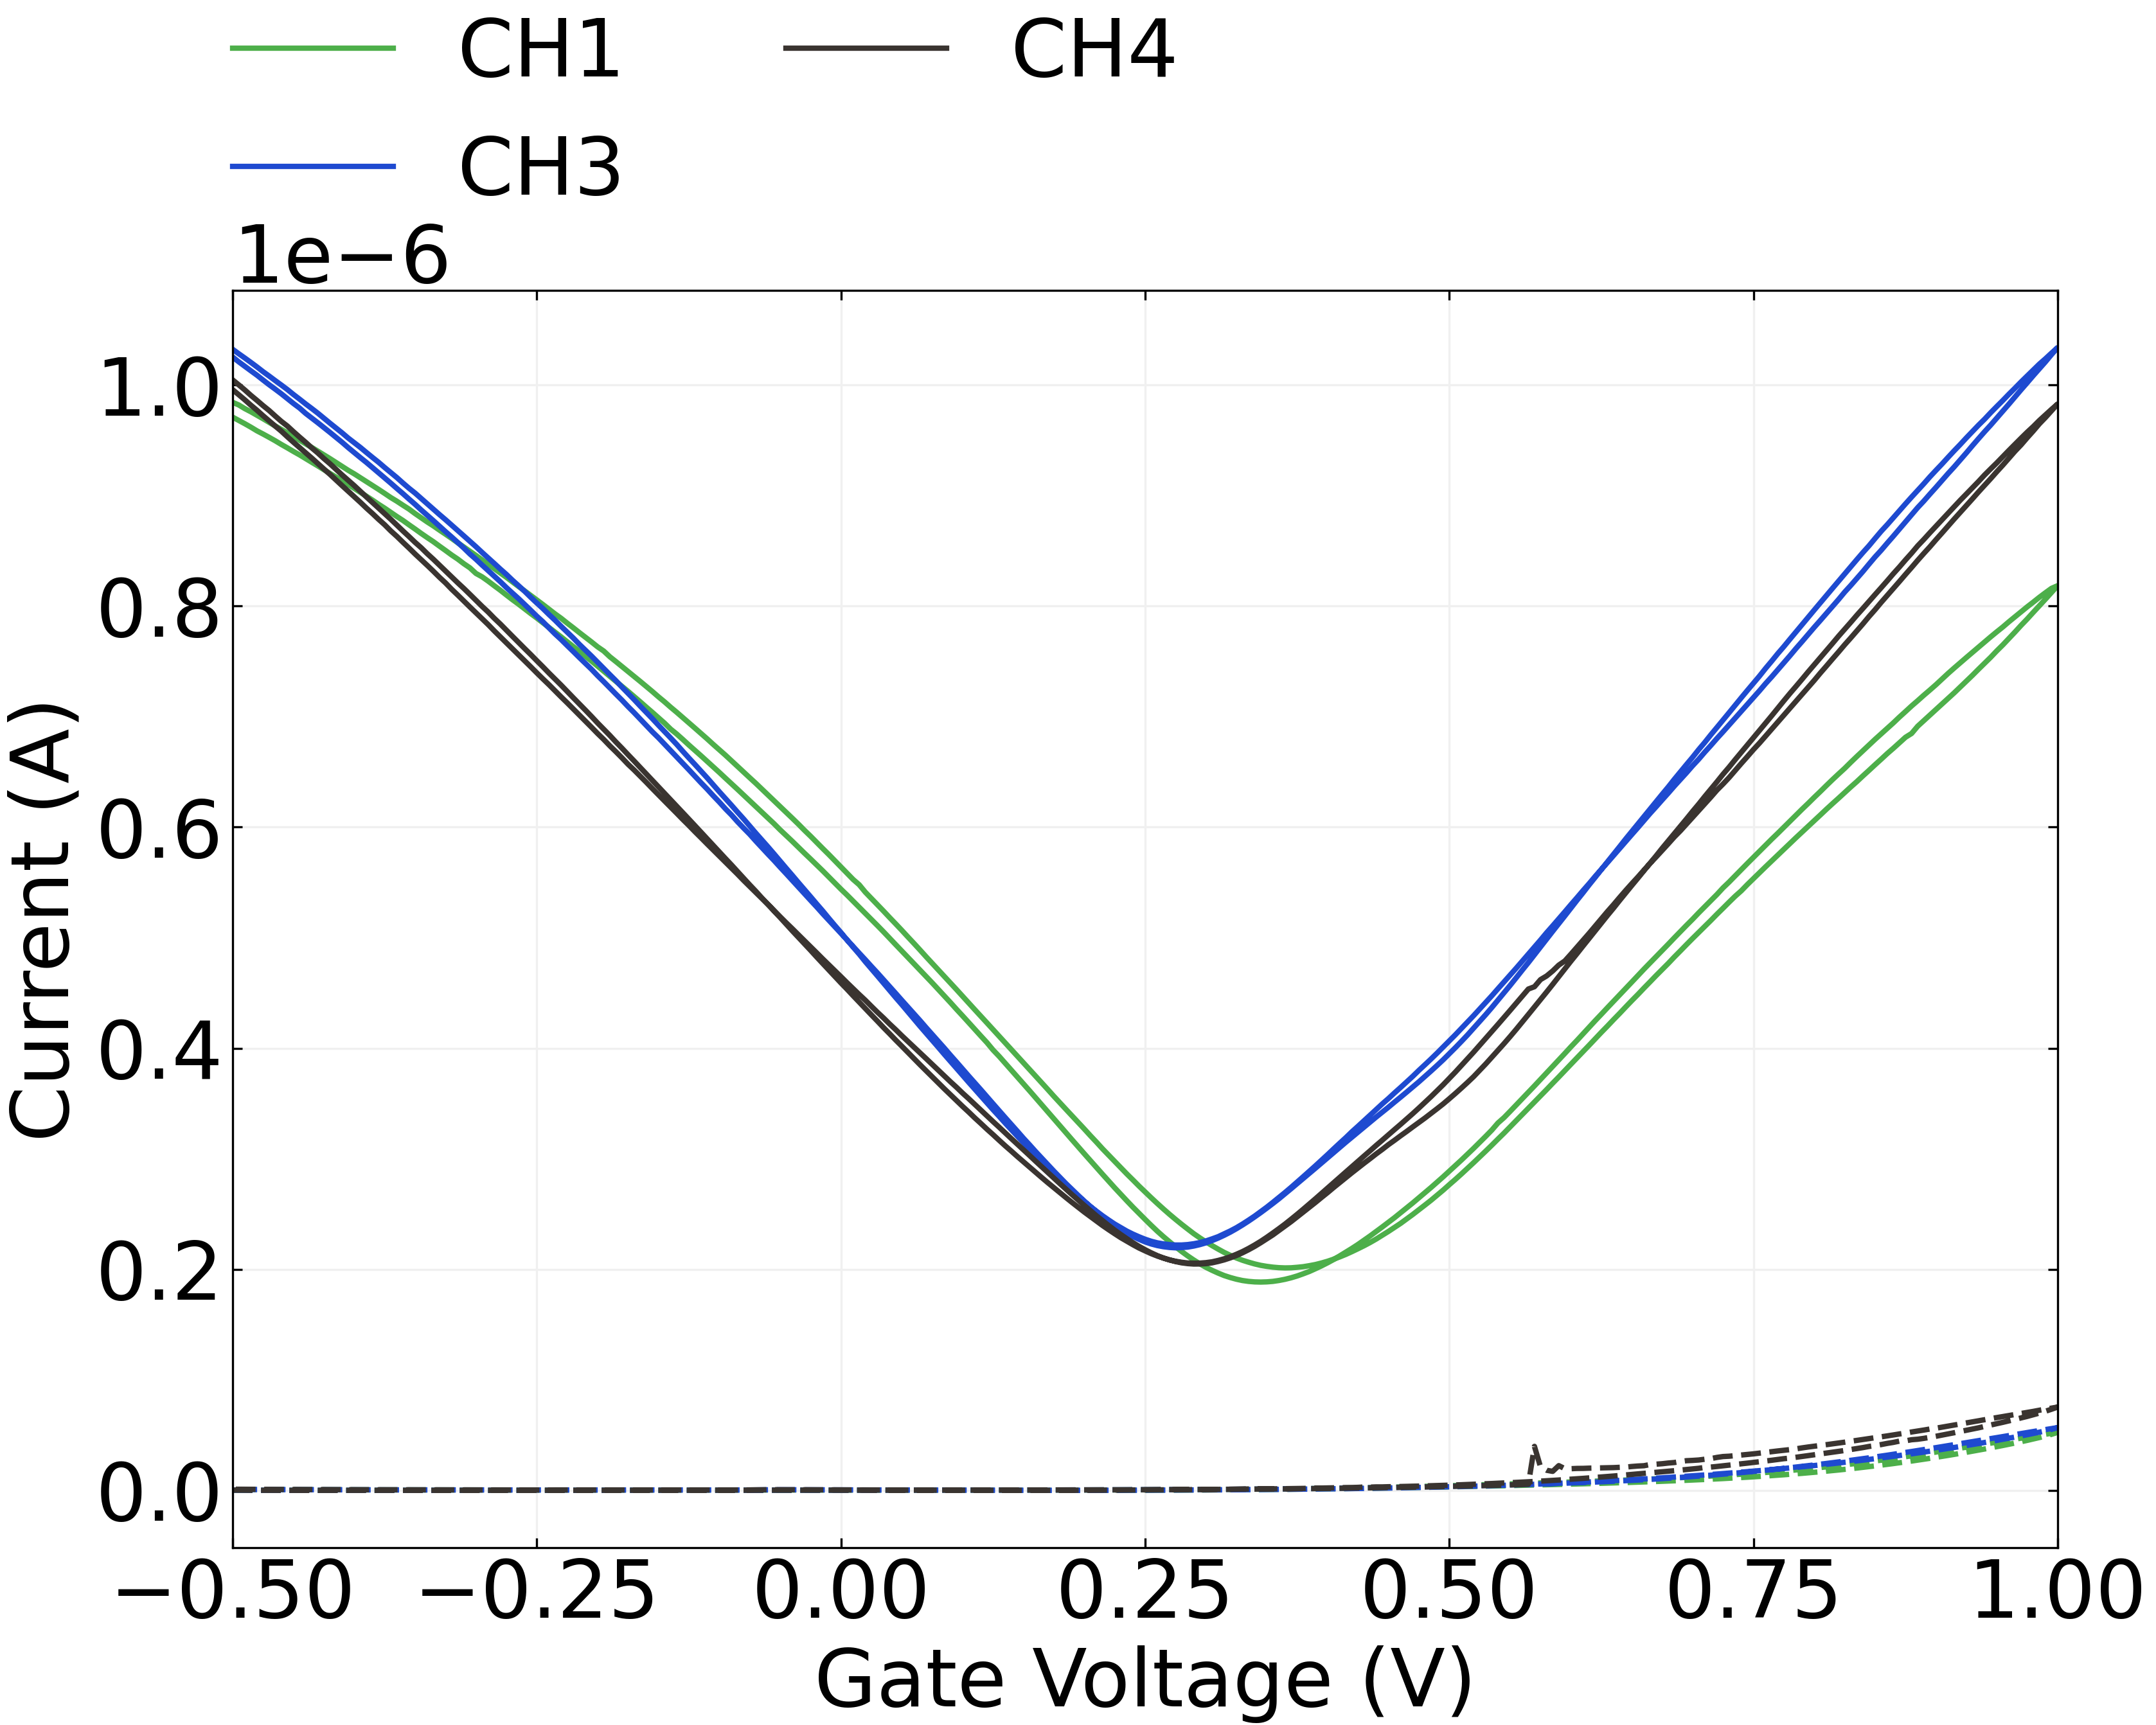
\includegraphics{./figures/ch5/JG098_pristine_TXLG01_5mVstep_220920_norinse.png}

}

}

\subcaption{\label{fig-y-voltage}}
\end{minipage}%

\caption{\label{fig-pristine-graphene}These liquid-gated transfer sweeps
show the transfer characteristics of the channels from two
AZ\(^\circledR\) 1518 encapsulated graphene devices upon initial
exposure to 1XPBS in (a) and (b). (b) and (e) after being coated in
1XPBS for 1 hour, and (c) and (f) after the device was rinsed and buffer
in the well was replaced with new 1XPBS. This procedure was followed to
examine the impact of 1XPBS on the electrical behaviour of the graphene
devices. The device in (d-f)}

\end{figure}

Graphene devices were electrically characterised in the manner described
in \textbf{?@sec-electrical-characterisation} and analysed using the
Python code discussed in
Section~\ref{sec-field-effect-transistor-analysis}.

\hypertarget{tbl-graphene-parameters}{}
\begin{table}
\caption{\label{tbl-graphene-parameters}Average on-off ratio and Dirac point for AZ® 1518 encapsulated
liquid-gated graphene transistor channels at various stages of exposure
to 1XPBS. Electrical characteristics were taken of 6 channels total, 3
each from two devices. }\tabularnewline

\centering
\begin{tabular}{lccc}
\toprule
 & 1XPBS: Initial & 1XPBS: After 1 hr & 1XPBS: Rinse\\
\midrule
On-Off Ratio (arb.) & 5.1 ± 0.3 & 5.0 ± 0.7 & 5.0 ± 0.6\\
Dirac Point Voltage (V) & 0.28 ± 0.04 & 0.31 ± 0.03 & 0.28 ± 0.02\\
\bottomrule
\end{tabular}
\end{table}

Figure~\ref{fig-pristine-graphene} shows liquid-gated transfer
characteristics of a single graphene device with three working channels.
This device was fabricated prior to Jun 2021. This device exhibits the
ambipolar characteristics typical of liquid-gated graphene devices
\autocite{Heller2009a,Heller2010,Xia2010,Kireev2017}. As with the carbon
nanotube network devices, leakage current remained below \(\sim\) 1
\(\times\) \(10^{-7}\) V across both the forward and reverse sweep.
Device channels were measured on exposure to 1XPBS, after exposure to
1XPBS for one hour and after the device surface was rinsed and 1XPBS was
replaced in the well. Table~\ref{tbl-graphene-parameters} shows that the
on-off ratio and Dirac point voltage of graphene device were highly
consistent before and after exposure to 1XPBS, indicating the presence
of 1XPBS had minimal impact on these key parameters. Exposure to 1XPBS
does not appear to impact the appearance of double-minima when
double-minima are present.

\hypertarget{sec-dummy-sensing}{%
\section{Salt Concentration Sensing with Phosphate Buffered
Saline}\label{sec-dummy-sensing}}

-nLOF2020 resist being used leads to devices with less drift!!

\appendix
\addcontentsline{toc}{part}{Appendices}

\hypertarget{sec-photolithography}{%
\chapter{Photolithography}\label{sec-photolithography}}

\begin{figure}

{\centering 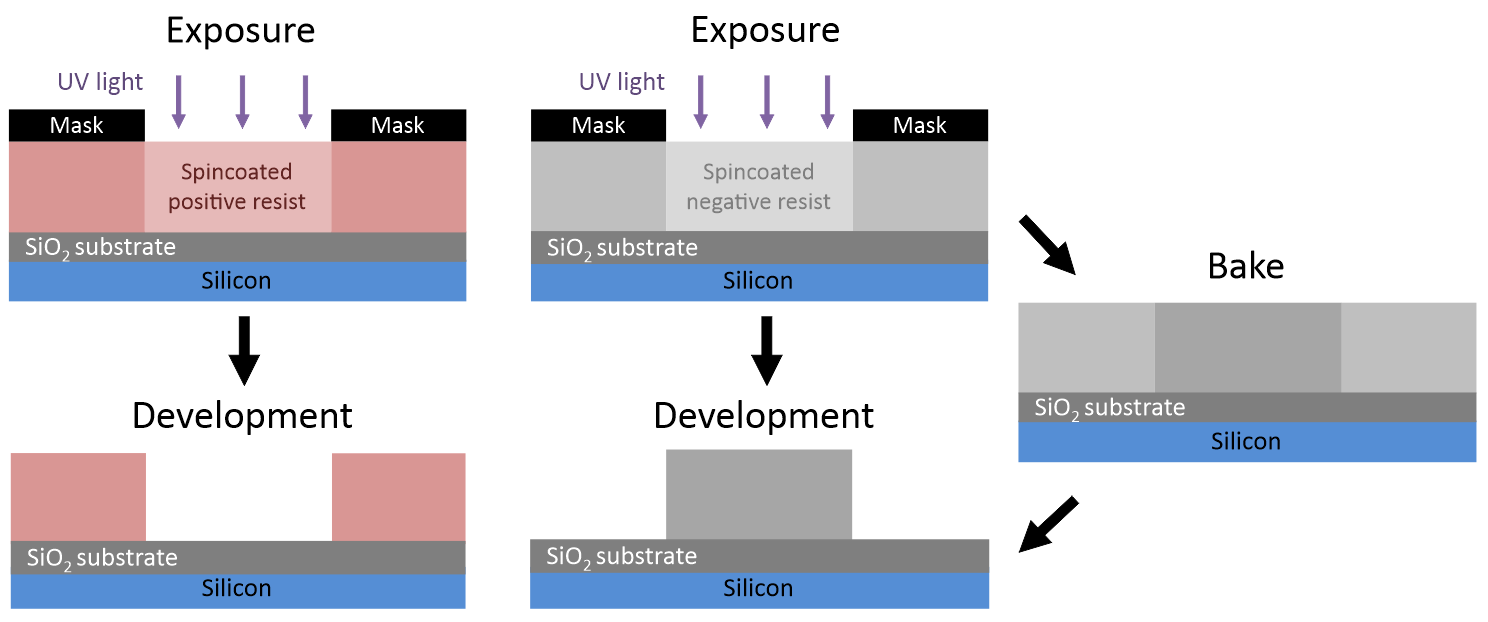
\includegraphics{./figures/app1/positive-negative-photolithography.png}

}

\caption{\label{fig-photolithography-types}A side-view comparison of
generic photolithography processes for positive and negative resists in
the ideal case. Photolithography with a positive resist requires a
single softbake step before exposure, while for negative resists a
second baking step is required after exposure (Thicknesses shown not to
scale).}

\end{figure}

This section details some of the standard photolithography procedures
used in the device fabrication processes detailed in
\textbf{?@sec-fabrication}. Photoresists, also referred to here as
``resists'', are UV light-sensitive polymeric resins used for
photolithography. Both positive and negative photoresists were used in
various fabrication processes. Positive resists are made soluble in
alkalines by UV light exposure, meaning exposed areas are removed in the
development process. Conversely, negative resists are cross-linked by
exposure and a post-exposure bake step. The unexposed areas of the
negative resist are then removed in the development process
\autocite{Microchemicals}. Figure~\ref{fig-photolithography-types} gives
a visual representation of these differences.

\begin{figure}

\begin{minipage}[t]{0.47\linewidth}

{\centering 

\raisebox{-\height}{

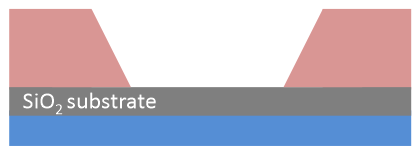
\includegraphics{./figures/app1/overcut-profile.png}

}

}

\subcaption{\label{fig-overcut-profile}Overcut profile of a positive
resist}
\end{minipage}%
%
\begin{minipage}[t]{0.05\linewidth}

{\centering 

~

}

\end{minipage}%
%
\begin{minipage}[t]{0.47\linewidth}

{\centering 

\raisebox{-\height}{

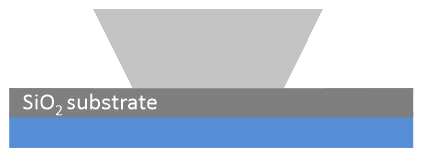
\includegraphics{./figures/app1/undercut-profile.png}

}

}

\subcaption{\label{fig-undercut-profile}Undercut profile of a negative
resist}
\end{minipage}%

\caption{\label{fig-photolithography-profiles}Two different resist
profiles seen for different types of photoresist. Each profile has had
the central region of the substrate exposed to UV light prior to
development. The undercut profile is ideal for thin-film metal
deposition and subsequent patterned removal, known as ``lift-off''.}

\end{figure}

The specific photoresist selected for photolithography depends on the
specific use case. The types used in this thesis are positive and
negative AZ\(^\circledR\) photoresists (AZ\(^\circledR\) 1518,
Microchemicals GmbH; AZ\(^\circledR\) nLOF 2020, Microchemicals GmbH)
and SU-8 (SU8-2150, Kayaku Advanced Materials, formerly Microchem). The
AZ\(^\circledR\) resists used here have a minimum film thickness of
\(1.5\textrm{ } \mu \textrm{m}\) \autocite{Microchemicals}, while the
SU8-2150 has a minimum film thickness of
\(0.5\textrm{ } \mu \textrm{m}\) \autocite{Kayaku}. Positive resists
which have not been thermally crosslinked will soften at higher
temperatures (\(\gtrsim 100^\circ\)C for AZ\(^\circledR\) 1518), leading
to a rounded profile. This is not the case for negative resists, which
are more thermally stable \autocite{Microchemicals}. Each resist
therefore has a different cross-section profile, as shown in
Figure~\ref{fig-photolithography-profiles}.

If metal deposition is performed on a positive resist, some metal can
collect on the outwardly-sloped sidewalls of the resist (see
Figure~\ref{fig-photolithography-profiles}) which forms significant
spikes on the edges of the deposited metal upon lift-off. On the other
hand, metal cannot collect on top of the inwardly-sloped negative
profile sidewalls, which avoids the formation of large edge spikes.
Therefore, the negative resist profile is more suited to metal or metal
oxide deposition and lift-off processes, though the process is more
sensitive to human error due to requiring more processing steps than
positive resist \autocite{Microchemicals}. Finally, when it is suitably
processed SU-8 is considered to be more stable and biocompatible than
other photoresists \autocite{Albarghouthi2022}. It is especially
biocompatible when chemically modified via processes such as isopropanol
sonication and O\(_2\) plasma treatment \autocite{Chen2021}.

All photolithographic exposure was performed using a Karl Suss MJB3
Contact Aligner with a USHIO super-high pressure 350 W mercury lamp
(USH-350DS, Japan). When performing photolithography, the intensity
reading from the aligner was \(20.8-24.2\) mW/cm\(^2\) (Note however
that an external photometer reading at 400 nm found an intensity output
of 17.2 mW/cm\(^2\) when the aligner read 21.0 mW/cm\(^2\)).

In general, photolithography procedures should be performed under yellow
lighting, as light wavelengths from \(320-450\) nm can promote reactions
in the photoresist used. Aging of photoresist over time can also
significantly affect the photolithography process, and therefore all
processes should be re-optimised regularly over time to give the desired
result \autocite{Microchemicals}. The range in processing times for some
steps of the processes used here are largely due to the effects of aging
on the photoresist.

The step-by-step processes for each resist are detailed in the
subsequent sections.

\hypertarget{azcircledr-1518-photoresist}{%
\section{\texorpdfstring{AZ\(^\circledR\) 1518
photoresist}{AZ\^{}\textbackslash circledR 1518 photoresist}}\label{azcircledr-1518-photoresist}}

\begin{enumerate}
\def\labelenumi{\arabic{enumi}.}
\item
  Spincoat at a final speed of 4000 rotations per minute (rpm) for 1
  minute, with an initial acceleration of 500 rpm/s (notes: clean the
  substrate with acetone, isopropanol (IPA) and nitrogen before
  spincoating; use only the minimum amount of photoresist required to
  fully cover the wafer surface; avoid any gaps or bubbles in the
  photoresist).
\item
  Softbake \(2-4\) minutes at \(95^\circ\)C on the hotplate (2 min for
  individual devices, 4 min for a quarter wafer)
\item
  Mask expose for \(10-12\) s (note: clean mask with acetone/IPA and
  N\(_2\) dry before use)
\item
  Develop with 3 parts AZ\(^\circledR\) 326 (2.38 \% TMAH metal-ion free
  developer, Microchemicals GmbH) in 1 part deionised (DI) water for
  \(30-45\) s (note: rinse for \(10-15\) s in one development solution,
  then perform the rest of the development in clean developer for a
  cleaner profile; lightly agitate the solution throughout the
  development process)
\item
  Rinse device for 30 s in DI water to remove excess developer, then dry
  under nitrogen
\end{enumerate}

\hypertarget{azcircledr-nlof-2020-photoresist}{%
\section{\texorpdfstring{AZ\(^\circledR\) nLOF 2020
photoresist}{AZ\^{}\textbackslash circledR nLOF 2020 photoresist}}\label{azcircledr-nlof-2020-photoresist}}

\begin{enumerate}
\def\labelenumi{\arabic{enumi}.}
\item
  Spincoat at final speed of 3000 rotations per minute (rpm) for 1
  minute, with an initial acceleration of 500 rpm/s (notes: clean the
  substrate with acetone, isopropanol (IPA) and nitrogen before
  spincoating; avoid any gaps or bubbles in the photoresist)
\item
  Softbake for precisely 60 s at \(110^\circ\)C on the hotplate
\item
  Mask expose for \(2.7-3\) s (note: clean mask with acetone/IPA and
  N\(_2\) dry before use)
\item
  Post-exposure bake for precisely 60 s at \(110^\circ\)C on the
  hotplate to cross-link exposed resist
\item
  Develop with 3 parts AZ\(^\circledR\) 326 in 1 part DI water for
  \(60-70\) s (note: rinse for 30 s in one development solution, then
  perform the rest of the development in clean developer for a cleaner
  profile; lightly agitate the solution throughout the development
  process)
\item
  Rinse device for 30 s in DI water to remove excess developer, then dry
  under nitrogen
\end{enumerate}

\hypertarget{su8-2150-photoresist}{%
\section{SU8-2150 photoresist}\label{su8-2150-photoresist}}

\begin{enumerate}
\def\labelenumi{\arabic{enumi}.}
\item
  SU-8 was diluted in cyclopentanone until viscosity was low enough to
  spincoat on substrate and then sonicated at \(50^\circ\)C for \(3-4\)
  hours (Note: The dilution ratio used was \textasciitilde1 part SU-8 to
  5 parts cyclopentanone. However, the age of the SU-8 may mean that
  significant evaporation had occurred prior to use, and the amount of
  SU-8 actually present is underrepresented by this ratio)
\item
  Spincoat first with a final speed of 500 rpm (acceleration 500 rpm/s)
  for 10 seconds, followed by spincoating at 4000 rpm (acceleration 7500
  rpm/s) for 40 s.
\item
  Softbake for 10 minutes at \(95^\circ\)C on the hotplate
\item
  Mask expose for \(6-8\) s (note: clean mask with acetone/IPA and
  N\(_2\) dry before use)
\item
  Post-exposure bake for 10 minutes at \(95^\circ\)C on the hotplate to
  cross-link exposed resist
\item
  Develop with SU-8 developer (Kayaku Advanced Materials, formerly
  Microchem) for \(10-15\) s, then clean in IPA for 30 s, repeat this
  step once then dry under nitrogen (note: lightly agitate the solution
  throughout the development process)
\end{enumerate}

\hypertarget{sec-python}{%
\chapter{Python Code for Data Analysis}\label{sec-python}}

\hypertarget{code-repository}{%
\section{Code Repository}\label{code-repository}}

The code used for general analysis of field-effect transistor devices in
this thesis was written with Python 3.8.8. Contributors to the code used
include Erica Cassie, Erica Happe, Marissa Dierkes and Leo Browning. The
code is located on GitHub and the research group OneDrive, and is
available on request.

\hypertarget{sec-histogram-analysis}{%
\section{Atomic Force Microscope Histogram
Analysis}\label{sec-histogram-analysis}}

The purpose of this code is to analyse atomic force microscope (AFM)
images of carbon nanotube networks in .xyz format taken using an atomic
force microscope and processed in Gwyddion (see
\textbf{?@sec-afm-characterisation}). It was originally designed by
Erica Happe in Matlab, and adapted by Marissa Dierkes and myself for use
in Python.

\begin{equation}\protect\hypertarget{eq-lin-combo-gaussian}{}{
f(x) = k_1\exp{\Bigg(-\frac{{(x-m_1)}^{2}}{{2s_1}^{2}}\Bigg)} + k_2\exp{\Bigg(-\frac{{(x-m_2)}^{2}}{{2s_2}^{2}}\Bigg)} + ...
}\label{eq-lin-combo-gaussian}\end{equation}

The .xyz data is initially sorted into bins with 0.15 nm size. The bin
with the maximum number of counts is set at 0 nm, as this peak
represents the mean of the surface roughness of the bare silicon. The
parameters \(m_i\), \(s_i\), \(k_i\) (i = 1, 2, 3) are used with
objective function Equation~\ref{eq-lin-combo-gaussian} to overlay the
data with normal distributions. These fitting parameters represent the
mean (m), standard deviation (s) and amplitude (k) of each normal
distribution. We can make approximations of some of these fitting
parameters using the histogram data.

\(k_1\) is taken to be the maximum y-value of the data being fitted,
\(m_1\) is set to zero (used as a point of reference) and \(s_1\) is
taken as one-third of the difference between \(m_1\) and the x-value of
the first datapoint where the y-value is greater than 1\% of \(k_1\)
(approximating one standard deviation). We find the distribution given
by these values using Equation~\ref{eq-lin-combo-gaussian}, and subtract
it from the existing dataset.

Then, using the analysis technique outlined by Vobornik \emph{et al.}
\autocite{Vobornik2023} in Gwyddion, we manually find estimates for the
mean \(m_2\) and standard deviation \(s_2\) of the carbon nanotube
bundle distribution. We then take \(k_2\) to be the maximum y-value of
this modified dataset, and \(m_1\) to be the x-value of the maximum
y-value. We then set \(k_2\) so that the height of the resulting
distribution at one standard deviation matches the height of the .xyz
data histogram. We take this distribution, and subtract it from the
existing dataset.

The code also allows for discretely binning continuous data from fitted
normal distributions and examining the proportion of counts above or
below a particular height. 2.9 nm is roughly where 2 bundles with
average size 1.45 nm can start to be present, and is used as an estimate
of the boundary value between single-tube bundle diameters and
multi-tube bundle diameters.

\hypertarget{sec-field-effect-transistor-analysis}{%
\section{Field-Effect Transistor
Analysis}\label{sec-field-effect-transistor-analysis}}

The purpose of this code is to analyse electrical measurements taken of
field-effect transistor (FET) devices. Electrical measurements were
either taken from the Keysight 4156C Semiconductor Parameter Analyser,
National Instruments NI-PXIe or Keysight B1500A Semiconductor Device
Analyser as discussed in \textbf{?@sec-electrical-characterisation}; the
code is able to analyse data taken from all three measurement setups.
The code consists of three related but independent modules: the first
analyses and plots sensing data from the FET devices, the second
analyses and plots transfer characteristics from channels across a
device, and the third compares individual channel characteristics before
and after a modification or after each of several modifications. These
modules were designed collaboratively by myself and Erica Cassie over
GitHub using the Sourcetree Git GUI.

\begin{equation}\protect\hypertarget{eq-lin-combo-exp-decay}{}{
f(x) = k_1\exp{\Bigg(-\frac{t}{{\tau}_{1}}\Bigg)} + k_2\exp{\Bigg(-\frac{t}{{\tau}_{2}}\Bigg)} + ... + c
}\label{eq-lin-combo-exp-decay}\end{equation}

\hypertarget{vapour-delivery-system}{%
\chapter{Vapour Delivery System}\label{vapour-delivery-system}}

\hypertarget{technical-notes}{%
\section{Technical Notes}\label{technical-notes}}

Two LabView Virtual Instruments (VIs) were adapted from pre-existing VIs
for operating the mass flow controllers and monitoring vapour flow into
the device chamber, as well as monitoring temperature and humidity in
the vapour delivery system's manifold. These VIs were named ``\,'' A
third VI was developed in parallel which combined the first two Virtual
Instruments, alongside allowing the sequence of values to control the
mass flow controllers.

From Honours report: ``\,``\,'' Figure 12 gives the right side of the
front panel of the LabView VI sample with vapour.VI, which letsus preset
an autonomously-performed vapour sensing sequence. Each row in each
array module corresponds to a differennest step in this sequence. The
`howManySteps' module lets us set how many of these steps are performed.
The `Durations Array' module determines the length of time in seconds
each step is performed over. The `Carrier Flows Array' and `Dilution
Flows Array' modules let us set the carrier flow and dilution flow,
respectively, in standard cubic centimetres per minute (sccm) through
the gas rig at each step. The carrier flow pushes analyte vapour into
the vapour-sensing device chamber, while dilution flow is used to modify
the flow behaviour of the analyte vapour entering the chamber. The
vapour sensing sequence as depicted in Figure 12 was used for all vapour
sensing runs in this investigation. At the end of the sequence, the data
collected about the vapour sensing process was saved as an .lvm file.
``\,``\,''

\hypertarget{future-improvements}{%
\section{Future Improvements}\label{future-improvements}}


\backmatter
\printbibliography


\end{document}
